% concatenated from neurips_2024.tex
\PassOptionsToPackage{table}{xcolor}

\documentclass{article}

% if you need to pass options to natbib, use, e.g.:
%\PassOptionsToPackage{numbers, compress}{natbib}
% before loading neurips_2024


% ready for submission
\usepackage[nonatbib, preprint]{neurips_2024}

\begin{filecontents*}{biblatex-dm.cfg}
% This is a placeholder so biblatex won’t complain on arXiv.
\end{filecontents*}


% to compile a preprint version, e.g., for submission to arXiv, add add the
% [preprint] option:
%     \usepackage[preprint]{neurips_2024}


% to compile a camera-ready version, add the [final] option, e.g.:
%     \usepackage[final]{neurips_2024}


% to avoid loading the natbib package, add option nonatbib:
%\usepackage[nonatbib]{neurips_2024}
\usepackage[
  backend=biber,       % (or 'bibtex' if you prefer, but biber is recommended)
  style=alphabetic,    % use the alphabetic (alpha) label format
]{biblatex}
\addbibresource{references.bib}
%\defcitealias{de2024robust}   {de Frutos et al.\,(2024\textit{a})}
%\defcitealias{de2024training}{de Frutos et al.\,(2024\textit{b})}


\usepackage[utf8]{inputenc} % allow utf-8 input
\usepackage[T1]{fontenc}    % use 8-bit T1 fonts
\usepackage{hyperref}       % hyperlinks
\usepackage{url}            % simple URL typesetting
\usepackage{booktabs}       % professional-quality tables
\usepackage{pgfplots}      % for axis environment
\usepackage{multirow}       % for multirow cells in tables
\usepackage{amsfonts}       % blackboard math symbols
\usepackage{nicefrac}       % compact symbols for 1/2, etc.
\usepackage{microtype}      % microtypography
\usepackage{amsmath}
\usepackage{amsthm}
\usepackage{amssymb}
\usepackage{comment}
\usepackage{subcaption}
\usepackage{graphicx}
\usepackage{booktabs}
%\usepackage[table]{xcolor}
\usepackage{siunitx}
\usepackage{venndiagram}
\usepackage{tikz}
\usepackage[export]{adjustbox}
\usepackage{comment}
\usepackage{algorithmic}
%\usepackage{algpseudocode}
\usepackage{algorithm}
\usepackage{setspace}
\usepackage{enumitem}
\usepackage{tabularx}
\usepgfplotslibrary{groupplots}

\usepackage{siunitx}      % for S columns
\sisetup{
  detect-mode,            % make S honor math/text mode
  separate-uncertainty=true % render “±” for uncertainties
}

% Define a math‐mode left‐aligned column
\newcolumntype{M}{>{$}l<{$}}

\newcommand{\commentPablo}[1]{\textbf{\textcolor{black}}}

\newcommand{\abs}[1]{\left\lvert#1\right\rvert}
\newcommand{\sign}{\operatorname{sign}}
\newcommand{\scalarprod}[2]{\langle #1, #2 \rangle}
\newcommand{\normdist}[2]{\mathcal{N}(#1, #2)}
\newcommand{\boldnum}[1]{\mathbf{#1}}
\newcommand{\triplenorm}[1]{%
  \left\lVert\!\!\left\lVert\!\!\left\lVert #1 
  \right\rVert\!\!\right\rVert\!\!\right\rVert
}

\newtheorem{definition}{Definition}[section]
\newtheorem{theorem}{Theorem}[section]
\newtheorem{lemma}{Lemma}[section]
\newtheorem{corollary}{Corollary}[section]
\newtheorem{remark}{Remark}[section]

\newcommand{\jose}[1]{\textcolor{red}{#1}}
\newcommand{\jm}{\textcolor{cyan}}

\captionsetup[subfigure]{%
  justification=centering,
  font=small,
  labelfont=bf,
  skip=1pt
}




%\title{Bernstein-Based $L^2$-Projection Loss \\A Convex, Likelihood-Free Divergence for Implicit Generative Training}

%\title{%
%  Bernstein‐Based $L^2$‐Projection Loss\\
%  A Convex Divergence with Explicit Density Expression for Implicit Generative Models
%}

%\title{%
%Bernstein-Based $L^2$-Projection Loss:\\
%  Convex Divergence with Explicit Density for Implicit Generative Models
%}

\title{Explicit Density Approximation for Neural Implicit Samplers Using a Bernstein-Based Convex Divergence}


% The \author macro works with any number of authors. There are two commands
% used to separate the names and addresses of multiple authors: \And and \AND.
%
% Using \And between authors leaves it to LaTeX to determine where to break the
% lines. Using \AND forces a line break at that point. So, if LaTeX puts 3 of 4
% authors names on the first line, and the last on the second line, try using
% \AND instead of \And before the third author name.


\author{%
  José Manuel de Frutos\thanks{Corresponding author: jofrutos@ing.uc3m.es} \\
  Universidad Carlos III\\
  \And
  Manuel A. Vázquez\\
  Universidad Carlos III\\
  % \texttt{email} \\
  \AND
  Pablo M. Olmos\\
  Universidad Carlos III\\
  % \texttt{email} \\
  \And
  Joaquín Míguez\\
  Universidad Carlos III\\
  % \texttt{email} \\
}

\makeatletter
  % 1) save the real \addcontentsline once and for all
  \let\saved@addcontentsline\addcontentsline

  % 2) suppress TOC entries by redefining \addcontentsline to gobble 3 args
  \newcommand\suppressTOCentries{%
    \renewcommand{\addcontentsline}[3]{}%
  }

  % 3) restore the original
  \newcommand\restoreTOCentries{%
    \let\addcontentsline\saved@addcontentsline%
  }
\makeatother


\begin{document}


\maketitle

\suppressTOCentries
\begin{abstract}

Rank-based statistical metrics, such as the invariant statistical loss (ISL), have recently emerged as robust and practically effective tools for training implicit generative models. In this work, we introduce dual-ISL, a novel likelihood-free objective for training implicit generative models that interchanges the roles of the target and model distributions in the ISL framework, yielding a convex optimization problem in the space of model densities. We prove that the resulting rank-based discrepancy $d_K$ is i) continuous under weak convergence and with respect to the $L^1$ norm, and ii) convex in its first argument—properties not shared by classical divergences such as KL or Wasserstein distances. Building on this, we develop a theoretical framework that interprets $d_K$ as an $L^2$-projection of the density ratio $q = p/\tilde p$ onto a Bernstein polynomial basis, from which we derive exact bounds on the truncation error, precise convergence rates, and a closed-form expression for the truncated density approximation. We further extend our analysis to the multivariate setting via random one-dimensional projections, defining a sliced dual-ISL divergence that retains both convexity and continuity. We empirically show that these theoretical advantages translate into practical ones. Specifically, across several benchmarks dual-ISL converges more rapidly, delivers markedly smoother and more stable training, and more effectively prevents mode collapse than classical ISL and other leading implicit generative methods—while also providing an explicit density approximation. 

\end{abstract}

\section{Introduction}

Implicit generative models are a class of models that learn to generate data samples without explicitly modeling the underlying probability distribution \cite{mohamed2016learning}, enabling flexible modeling of high-dimensional data across vision (e.g., DCGAN \cite{radford2015unsupervised}), audio (e.g., WaveGAN \cite{donahue2018adversarial}), and text domains (e.g., SeqGAN \cite{yu2017sequence}). Instead of directly estimating the data distribution, these models learn a mapping from a simple input distribution (such as a multivariate Gaussian) to the data space through a deterministic or stochastic function. A prominent example is the generator in a Generative Adversarial Network (GAN) \cite{goodfellow2014generative}, which transforms random noise vectors into realistic data samples. The generator is trained in tandem with a discriminator that learns to distinguish real data from generated data, providing feedback that guides the generator to improve. Unlike explicit models, implicit models do not require tractable likelihoods, allowing them to generate high-quality samples even when the data distribution is complex or high-dimensional.

The Invariant Statistical Loss (ISL) is a rank-based loss function recently proposed in \cite{de2024training} that compares the empirical order statistics of samples from the data and from the implicit generative model. In this work, we introduce \textbf{dual-ISL}, a novel likelihood-free objective obtained by swapping the roles of the data and model distributions within the ISL framework. Remarkably, the induced discrepancy \(d_K\) admits a fully \emph{explicit closed-form density approximation}: it is exactly the \(L^2\)–projection of the density ratio
\[
q(x)\;=\;\frac{p_{\mathrm{target}}(x)}{p_{\mathrm{model}}(x)}, 
\qquad
x = F_{\mathrm{target}}^{-1}(t),\;t\in[0,1],
\]
onto the space of dual-Bernstein polynomials of degree \(K\) \cite{lorentz2012bernstein,jiittler1998dual}. Writing
\[
q_K(x)
=\sum_{n=0}^K \mathbb{Q}_K(n)\,\tilde b_{n,K}\bigl(F_{\mathrm{target}}(x)\bigr)
\]
with computable coefficients \(\{\mathbb{Q}_K(n)\}\) immediately yields
\[
p_{\mathrm{model}}(x)\;\approx\;\frac{p_{\mathrm{target}}(x)}{q_K(x)}.
\]
This explicit representation not only provides analytic error bounds via Bernstein approximation theory and ensures convexity over the space of densities, but also enables efficient density evaluation without auxiliary sampling and provable convergence rates inherited from polynomial approximation. By marrying likelihood-free training with a tractable, closed-form density, dual-ISL bridges a critical gap—offering both rigorous theory and practical stability in implicit generative modeling. Moreover, this rank-based construction directly parallels the univariate optimal transport problem: matching order statistics via the probability–integral transform recovers the Monge map and yields the \(p\)-Wasserstein distance \cite{villani2008optimal}. Dual-ISL extends this perspective by providing an explicit, closed-form polynomial approximation of the density ratio—complete with convexity guarantees and convergence rates—rather than only a transport map.

% Implicit generative models define complex data distributions through sampling procedures rather than tractable likelihoods \cite{mohamed2016learning}, enabling flexible modeling of high-dimensional data across vision (e.g., DCGAN \cite{radford2015unsupervised}), audio (e.g., WaveGAN \cite{donahue2018adversarial}), and text domains (e.g., Diffusion-LM \cite{li2022diffusion}). Such models fall into several broad categories. Adversarial methods train a generator to fool a discriminator without ever evaluating likelihoods; flow-based architectures compose invertible mappings to permit exact density computation; diffusion and score-based processes learn to reverse a noise injection procedure via stochastic differential equations; energy-based models specify unnormalized energy functions and rely on MCMC for sampling; noise-contrastive estimation (NCE) converts density estimation into a classification problem; and autoregressive approaches factor joint distributions into sequential conditionals. Each paradigm navigates trade-offs between sample quality, density tractability, and computational cost.

% Generative Adversarial Networks (GANs) \cite{goodfellow2014generative} pioneered likelihood-free training by casting generation as a minimax game between a generator and a discriminator. Despite impressive sample quality, GANs suffer from non-convex objectives and training instability. The Wasserstein GAN (WGAN) introduced the Earth-Mover’s distance to stabilize gradients and improve convergence diagnostics \cite{arjovsky2017wasserstein}, while WGAN-GP replaced weight clipping with a gradient penalty for more robust Lipschitz enforcement \cite{gulrajani2017improved}. Spectral normalization (SN-GAN) constrains the discriminator’s Lipschitz constant via weight normalization, yielding more stable training with minimal overhead \cite{miyato2018spectral}. Finally, Moment-matching variants such as MMD-GAN replace the discriminator with a two-sample test based on the maximum mean discrepancy (MMD), aligning higher-order feature statistics between real and generated samples and even learning the kernel adversarially to boost expressiveness and stability. By casting training as a convex moment-matching problem in function space rather than a minimax game, MMD-GAN \cite{li2017mmd} typically yields smoother loss curves and reduced mode collapse compared to adversarial methods like SN-GAN. Beyond adversarial methods, diffusion‐based models—including DDPMs \cite{ho2020denoising} and score‐based approaches \cite{song2020score}—train a reverse noise process or score function to achieve high‐fidelity samples, at the expense of many sequential denoising steps.  Normalizing flows \cite{rezende2015variational}, by composing a chain of invertible transformations, offer exact likelihoods and one‐shot sampling, but their expressivity is limited by the requirement that each layer’s Jacobian remain tractable.


% % Beyond adversarial methods, diffusion probabilistic models such as Denoising Diffusion Probabilistic Models (DDPM) iteratively denoise samples through a learned reverse diffusion process to attain high sample fidelity at the cost of many inference steps \cite{ho2020denoising}. Score‐based generative models estimate data score functions and sample via stochastic differential equations, unifying and extending diffusion approaches without adversarial training \cite{song2020score}. Normalizing flows construct complex densities via sequences of invertible mappings, providing exact likelihood evaluation and efficient sampling but requiring careful architectural design to balance expressivity and tractability \cite{rezende2015variational}. Energy-based models assign unnormalized energy functions to data and sample via MCMC, offering flexible likelihood-free modeling at the expense of slower sampling \cite{du2019implicit}. Noise-contrastive estimation frames density learning as binary classification between data and noise, furnishing a consistent estimator for unnormalized models with moderate overhead \cite{gutmann2010noise}. Autoregressive models decompose joint distributions into products of conditionals over ordered components, yielding exact likelihoods but incurring sequential generation costs \cite{van2016pixel}.

% Despite this rich landscape, existing implicit objectives are often non-convex in the model parameters \cite{kodali2017convergence}, lack explicit density forms, or demand high sampling cost \cite{salimans2022progressive, song2020denoising}. In this work, we propose dual-ISL, a novel likelihood-free objective that swaps the roles of the model and target distributions within the Invariant Statistical Loss framework \cite{de2024training}, yielding a \emph{convex} optimization problem over model densities. Crucially, we show that the induced discrepancy \(d_K\) admits an \emph{explicit closed-form density approximation}: it corresponds to the \(L^2\)-projection of the density ratio
% \[
% q(x) \;=\;\frac{p_\text{target}(x)}{p_\text{model}(x)}, \qquad \text{where}\; x=F_{\text{target}}^{-1}(t), t\in[0,1]
% \]
% onto the space of dual-Bernstein polynomials of degree \(K\) \cite{lorentz2012bernstein, jiittler1998dual}. The resulting projected ratio
% \begin{align*}
%    q_{K}(x) =  \sum_{n=0}^{K} \mathbb{Q}_{K}(n) \,\tilde{b}_{n,K}(F_{\text{target}}(x)),
% \end{align*}
% with (computable) coefficients $\{\mathbb{Q}_{K}(n)\}$, yields an explicit model density \(p_{\text{model}}(x) \approx p_{\text{target}}(x)/q_K(x)\). This novel explicit representation affords analytic error bounds from Bernstein approximation theory, guarantees of convexity and continuity under weak convergence and \(L^1\) norms, efficient density evaluation without auxiliary sampling, and rigorous convergence rates derived from polynomial approximation properties. By combining likelihood‐free training with an explicit, closed-form density approximation, dual-ISL bridges a key gap in implicit generative modeling—offering both strong theoretical guarantees alongside practical training stability.

% \section{Introduction}

% In \cite{de2024training}, a novel method is introduced for training univariate implicit models that leverages a key property of rank statistics. Consider an ordered sequence  
% \begin{align*}
% r_1 < r_2 < \cdots < r_k,
% \end{align*} 
% of independent samples drawn from the generative model with probability density function (pdf) $\tilde{p}_{\theta}$. Define \(r_0=-\infty\) and \(r_{K+1}=\infty\), and let \(y\) be an independent sample from another pdf \(p\). When $\tilde{p}_{\theta}=p$, the probability that \(y\) falls in any interval \([r_{i-1}, r_i)\) is  
% \begin{align*}
% \mathbb{P}(r_{i-1} \leq y < r_i) = \frac{1}{K+1} \quad \text{for } i=1,\ldots,K+1,
% \end{align*} 
% as detailed in, e.g., \cite{rosenblatt1952remarks} or \cite{elvira2016adapting}. This invariant property holds for any continuously distributed data and can be exploited to design an objective function—termed the invariant statistical loss (ISL)—even when the true pdf \(p\) is unknown.

% In this work, we propose a novel algorithm that constructs the rank statistics by interchanging the roles of \(p\) and \(\tilde{p}\). Specifically, by sampling a fictitious dataset from \(\tilde{p}_{\theta}\) and comparing it against \(K\) samples from \(p\). In this setting, the ISL becomes convex in the space of model densities, enhancing its optimization properties. We then establish new continuity results for the defined discrepancy—results that traditional metrics like the Wasserstein distance and KL-divergence do not share.

% Next, we introduce a new theoretical framework that interprets the ISL as a $L^{2}$-projection of the ratio $q = \frac{p}{\tilde{p}_\theta}$  
% onto a Bernstein polynomial basis of degree $K$ \cite{lorentz2012bernstein}. The uniformity of the rank statistics guarantees that the ratio equals $1$ at the discretized points \(\{n/K\}_{n=0}^{K}\). This key property underlies the ISL approach is a likelihood-free inference method that employs density ratio comparisons for evaluation \cite{mohamed2016learning}, based on projections onto a Bernstein polynomial basis of grade $K$. This insight enables us to derive exact bounds on the truncation error of \(q\) when using \(K\) basis functions, as well as to establish precise convergence rates. Furthermore, it provides an explicit expression for the truncated quotient \(q_K\) in a Bernstein polynomial basis, thereby facilitating the efficient recovery of the true density. Finally, we extend our analysis to the multivariate setting using the one-dimensional projection scheme introduced in \cite{de2024robust}. As a result, we can derive convergence results based on \(K\) and further generalize the linear projection framework to non-linear schemes.


\section{The Invariant Statistical Loss (ISL)} \label{section: preliminaries}

We briefly review the invariant statistical loss (ISL) from \cite{de2024training}.  ISL is built on a simple rank statistic whose distribution is exactly uniform when two samples come from the same probability density function, and which varies continuously under $L^1$‐perturbations of the underlying densities.

\subsection{Rank statistic and uniformity}\label{sec:rank}

Let $\tilde y_1,\dots,\tilde y_K$ be i.i.d.\ samples from a univariate real distribution with pdf $\tilde{p}$, and let $y$ be a single sample independently drawn from another distribution with pdf $p$. Define the subset
\begin{align*}
\mathcal{A}_{K} 
\;:=\; 
\Bigl\{\tilde{y} \in \{\tilde{y}_{k}\}_{k=1}^{K} : \tilde{y} \leq y\Bigr\},
\end{align*}
and the \emph{rank statistic}
\begin{align}\label{eq: rank statistic}
     A_{K} 
     \;:=\; 
     \bigl|\mathcal{A}_{K}\bigr|,
 \end{align}
 i.e., $A_{K}$ counts how many samples in $\{\tilde{y}_1,\ldots,\tilde{y}_K\}$ lie at or below $y$. Then $A_{K}$ is a discrete random variable (r.v.) taking values in $\{0,1,\ldots,K\}$, and we denote its pmf by 
 \begin{align*}
     \mathbb{Q}_K:\{0,\ldots,K\}\to[0,1].
 \end{align*}
When the two pdfs $p$ and $\tilde{p}$ coincide, this pmf is exactly uniform \cite{de2024training}.
\begin{theorem}\label{thm:uniformity}
If $p = \tilde{p}$, then $A_{K}$ is uniformly distributed on $\{0,\ldots,K\}$, i.e.\ $\mathbb{Q}_{K}(n)=\tfrac{1}{K+1}$ for all $n \in \{0,\ldots,K\}$.
\end{theorem}

\subsection{ISL discrepancy}\label{sec:loss}
The ISL discrepancy quantifies the deviation of the pmf $\mathbb{Q}_{K}$ from the uniform law on $\{0,\dots,K\}$. To be specific, we define the discrepancy function
\begin{align}\label{eq:dK}
d_{K}(p,\tilde{p})
:= \dfrac{1}{K+1}\|\mathbb{Q}_{K} - \mathbb{U}_{K}\|_{\ell_{1}}= 
\frac{1}{K+1}\sum_{n=0}^{K}
\Bigl|\,
\tfrac{1}{K+1} 
\;-\; 
\mathbb{Q}_{K}(n)
\Bigr|= \dfrac{2}{K+1} \mathrm{TV}(\mathbb{Q}_{K}, \mathbb{U}).
\end{align}
where $\mathbb U_K$ is the uniform pmf on $\{0,\dots,K\}$ and $\mathrm{TV}(\cdot,\cdot)$ denotes total variation distance.
By Theorem~\ref{thm:uniformity}, $d_K(p,p)=0$ for all $K$.  Moreover, Theorem~\ref{thm:continuity} below, ensures that \(d_K(p,\tilde p)\) depends continuously on \(\tilde p\) in the \(L^1\) sense, while Theorem~\ref{thm:identifiability} guarantees that if \(d_K(p,\tilde p)=0\) for all \(K\), then \(\tilde p=p\) almost everywhere.  Hence, in the large-\(K\) limit, \(d_K\) behaves as a proper divergence, vanishing precisely when the two densities coincide.

\begin{theorem}[Continuity]\label{thm:continuity}
If $\|p - \tilde{p}\|_{L^1(\mathbb{R})}\,\le\,\epsilon,$ then for all $n\in \{0,\ldots,K\}$,
\begin{align*}
 \frac{1}{K+1}-\epsilon
 \;\;\le\;\;
 \mathbb{Q}_{K}(n)
 \;\;\le\;\;
 \frac{1}{K+1}+\epsilon.
\end{align*}
\end{theorem}

\begin{theorem}[Identifiability]\label{thm:identifiability}
Let $p,\tilde{p}$ be pdfs of univariate real r.v.s. If the rank statistic $A_{K}$ in \eqref{eq: rank statistic} is uniformly distributed on $\{0,\ldots,K\}$ for \emph{every} $K\in \mathbb{N}$, then $p=\tilde{p}$ almost everywhere.
\end{theorem}

Finally, when $\tilde p=\tilde p_\theta$ depends smoothly on a parameter vector ~$\theta$, one can show (under mild regularity assumptions) that $\theta\mapsto d_K(p,\tilde p_\theta)$ is continuous and differentiable, making it suitable for gradient‐based optimization (see Theorem 4 in \cite{de2024robust}). For full proofs and additional remarks, see \cite{de2024training,de2024robust}.  

% \subsection{Discrete uniform rank statistics}\label{Discrete uniform rank statistics}

% Let $\tilde{y}_1, \ldots, \tilde{y}_K$ be i.i.d.\ samples from a univariate real distribution with pdf $\tilde{p}$, and let $y$ be a single sample independently drawn from another distribution with pdf $p$. Define
% \[
% \mathcal{A}_{K} 
% \;:=\; 
% \Bigl\{\tilde{y} \in \{\tilde{y}_{k}\}_{k=1}^{K} : \tilde{y} \leq y\Bigr\},
% \]
% and the \emph{rank statistic}
% \begin{align}\label{eq: rank statistic}
%     A_{K} 
%     \;:=\; 
%     \bigl|\mathcal{A}_{K}\bigr|,
% \end{align}
% i.e., $A_{K}$ counts how many samples in $\{\tilde{y}_1,\ldots,\tilde{y}_K\}$ lie at or below $y$. Then $A_{K}$ is a discrete random variable taking values in $\{0,1,\ldots,K\}$, and we denote its pmf by
% \[
% \mathbb{Q}_K:\{0,\ldots,K\}\to[0,1].
% \]

% This pmf satisfies the following key fact.

% \begin{theorem}\label{theorem1}
% If $p = \tilde{p}$, then $A_{K}$ is uniformly distributed on $\{0,\ldots,K\}$, i.e.\ $\mathbb{Q}_{K}(n)=\tfrac{1}{K+1}$ for all $n \in \{0,\ldots,K\}$.
% \end{theorem}

% The next theorem extends the above to the case where $\tilde{p}$ \emph{approximately} equals $p$, implying that the \jm{pmf of} $A_{K}$ is continuous w.r.t. the $L^{1}$-norm. 

% \begin{theorem}\label{theorem2}
% If $\|p - \tilde{p}\|_{L^1(\mathbb{R})}\,\le\,\epsilon,$ then for all $n\in \{0,\ldots,K\}$,
% \[
%     \frac{1}{K+1}-\epsilon
%     \;\;\le\;\;
%     \mathbb{Q}_{K}(n)
%     \;\;\le\;\;
%     \frac{1}{K+1}+\epsilon.
% \]
% \end{theorem}

% Finally, if $A_{K}$ is uniformly distributed for every $K$, it forces $p=\tilde{p}$ everywhere. This result is established in \cite{de2024training} and is included here for completeness.

% \begin{theorem}\label{theorem4}
%     Let $p,\tilde{p}$ be pdfs of univariate real r.v.s. Suppose the rank statistic $A_{K}$ in \eqref{eq: rank statistic} is uniformly distributed on $\{0,\ldots,K\}$ for \emph{every} $K\in \mathbb{N}$. Then $p=\tilde{p}$ everywhere.
% \end{theorem}

% The theorems and proofs presented above, along with other remarks, are available in \cite{de2024robust}.

% %\begin{remark}
% %If $p$ and $\tilde{p}$ share compact support, variations of the above still hold for other $L^q$ norms, not just $L^1$; see \cite{brezis2011functional} for a classic argument involving H\"older's inequality.
% %\end{remark}

% \subsection{Summary of the Invariant Statistical Loss}

% Building on the previously introduced rank statistic Eq. \ref{eq: rank statistic}, \cite{de2024robust} introduces a new discrepancy function
% \begin{align*}
% d_{K}(p,\tilde{p}): C(\mathbb{R}) \times C(\mathbb{R}) \;\to\; [0,\infty),
% \end{align*}
% which quantifies the closeness of a continuous density \(\tilde{p}\) to a target density \(p\) on $\mathbb{R}$. The key idea is to compare the rank-based probability mass function \(\mathbb{Q}_{K}\) associated with the statistic \(A_{K}\) against the uniform probability mass function on \(\{0,\ldots,K\}\). Concretely,
% \begin{align*}
% d_{K}(p,\tilde{p})
% = \dfrac{1}{K+1}\|\mathbb{Q}_{K} - \mathbb{U}_{K}\|_{\ell_{1}}= 
% \frac{1}{K+1}\sum_{n=0}^{K}
% \Bigl|\,
% \tfrac{1}{K+1} 
% \;-\; 
% \mathbb{Q}_{K}(n)
% \Bigr|= \dfrac{2}{K+1} \mathrm{TV}(\mathbb{Q}_{K}, \mathbb{U}).
% \end{align*}

% The newly introduced loss function $d_{K}(p,\tilde{p})$ acts as a probability divergence in the limit $K\to\infty$, since $d_{K}(p,\tilde{p})=0$ for arbitrarily large $K$ if and only if $p=\tilde{p}$. In addition, $d_{K}(p,\tilde{p})$ is continuous with respect to the $L^{1}$-distance between $p$ and $\tilde{p}$. Furthermore, if the model density $\tilde{p}$ depends on parameters (e.g., through a generator $g_\theta$), continuity and Lipschitz assumptions on $g_\theta$ ensure that $d_{K}(p,\tilde{p}_\theta)$ inherits similar regularity with respect to $\theta$, making it amenable to gradient-based or subgradient-based optimization methods. In \cite{de2024robust}, the authors establish several properties of the newly introduced discrepancy measure \( d_{K}(p, \tilde{p}_{\theta}) \), demonstrating its suitability for machine learning applications. These properties pertain to the behavior of \( d_{K} \) within the parameter space, ensuring its effectiveness in optimization and model training processes (see  \cite[Theorem 4]{de2024training}).

\subsection{A surrogate for ISL optimization}

% Direct minimization of the divergence \(d_K(p, \tilde{p}_\theta)\) with respect to \(\theta\) is infeasible because the dependence of the empirical distribution \(\mathbb{Q}_K\) on \(\theta\) is unknown. Moreover, since \(d_K(p, \tilde{p}_\theta)\) is impractical for direct use, \cite{de2024robust} propose a surrogate loss function that is computationally tractable and can be optimized with respect to the network parameters \(\theta\) using standard gradient-based methods. Empirical evaluations in \cite{de2024robust} further demonstrate that the difference between the true loss and the surrogate is negligible. For a detailed explanation of the surrogate loss function's construction, please refer to \cite[Section 2.3]{de2024robust}.

Directly minimizing the divergence $d_K\bigl(p,\tilde p_\theta\bigr)$ with respect to the generator parameters $\theta$ is normally not feasible: the pmf $\mathbb{Q}_{K}$ has to be approximated empirically and its dependence on $\theta$ is unknown. To overcome this difficulty, \cite{de2024training} introduced a carefully designed surrogate loss that (i) closely tracks $d_K$, and (ii) admits gradient optimization via standard backpropagation. This surrogate is constructing by approximating the pmf of $\mathbb{Q}_{K}$ using  sigmoidal functions and a Gaussian kernel density estimator. In practice, training with the surrogate yields virtually identical performance to optimizing the true ISL, while remaining fully likelihood‐free and amenable to efficient stochastic optimization. For full details of the surrogate derivation, implementation, and bias‐variance trade‐offs, see \cite[Section 2.3]{de2024robust}.


\section{The dual-Invariant statistical loss} \label{section: new theoretical results about discrepancy measure}

By interchanging the roles of the data distribution \(p\) and the model distribution \(\tilde p\) in the ISL framework, we obtain a \emph{dual} objective that remains likelihood-free, but crucially becomes convex in the model pdf $\tilde{p}$.  

\subsection{Continuity and convexity of $d_{K}(p,\tilde{p})$}

Unlike most classical discrepancies, this rank‐based measure is \emph{weakly continuous}: if \(p_n\overset{w}{\longrightarrow} p\) weakly, then \(\lim_{n\to\infty}d_K(p_n,\tilde p)= d_K(p,\tilde p)\) (Theorem~\ref{thm:rankWeakConv} below).  In contrast, the Kullback–Leibler divergence does not enjoy weak continuity, and the Wasserstein and Energy distances require uniformly bounded moments to guarantee even this level of stability \cite[Section 5]{huster2021pareto}.  Finally, we show that \(d_K\) is convex in its first argument (Theorem~\ref{Theorem: Convexity in the First Argument}), yielding a tractable convex optimization problem in the space of densities.

A key insight in the continuity proof is that each probability mass $\mathbb{Q}_{K}(n)$, for $n=0,\ldots, K$, can be written as a continuous mixture of the binomial pmf's. Indeed, drawing \(K\) i.i.d.\ samples \(\tilde y_i\sim\tilde p\) and counting how many of them fall below \(y\) yields a \(\mathrm{Binomial}(K,\tilde F(y))\) distribution.  Since \(y\) itself is drawn from \(p\), one obtains \cite[Appendix 1]{de2024training}
\[
\begin{aligned}
\mathbb{Q}_K(n)&:=\int_{\mathbb{R}}h_{n}(y)\,p(y)\,\mathrm{d}y\,,\\
\text{where, }&\; h_{n}(y):=\binom{K}{n}\,\tilde F(y)^{n}\bigl(1-\tilde F(y)\bigr)^{K-n}\,,\quad n=0,1,\dots,K\,.
\end{aligned}
\]
and the bounded, continuous functions \(h_n\) then ensure weak continuity of \(\mathbb{Q}_K\) and hence of \(d_K\).  We formalize this argument in the following theorem.

%In particular, we prove that the ISL divergence is continuous with respect to the weak topology—a property that many classical divergences lack. For instance, the Kullback-Leibler divergence is not weakly continuous, and both the Wasserstein and Energy distances only exhibit continuity under the assumption of uniformly bounded moments (see \cite[Section 5]{huster2021pareto}).

% \begin{theorem}[Continuity of rank-based divergence under weak convergence]
% \label{thm:rankWeakConv}
% Let $\{p_n\}_{n \ge 1}$ be a sequence of pdfs on $\mathbb{R}$ that converges \emph{weakly} to a limiting pdf $p$. Suppose $\tilde{p}$ is a fixed reference density on $\mathbb{R}$, with a cdf $\tilde{F}(y)$. 
% For each integer $K \ge 1$, define the binomial mixture pmfs
% \begin{align*}
% \mathbb{Q}_K^{(n)}(m)
% =
% \int_{\mathbb{R}}
% \binom{K}{m}\,
% \bigl[\tilde{F}(y)\bigr]^m
% \bigl[1 - \tilde{F}(y)\bigr]^{K-m}
% \,p_n(y)\,\mathrm{d}y,
% \quad
% m=0,\dots,K,
% \end{align*}
% and
% \begin{align*}
% \mathbb{Q}_K(m)
% =
% \int_{\mathbb{R}}
% \binom{K}{m}\,
% \bigl[\tilde{F}(y)\bigr]^m
% \bigl[1 - \tilde{F}(y)\bigr]^{K-m}
% \,p(y)\,\mathrm{d}y.
% \end{align*}
% Then
% \begin{enumerate}
% \item[\textup{(i)}] Componentwise Convergence:
% If $p_n \Rightarrow p$ in the weak sense, then for each $m=0,\dots,K$,
% \begin{align*}
% \lim_{n\to\infty}
% \mathbb{Q}_K^{(n)}(m)
% =
% \mathbb{Q}_K(m).
% \end{align*}

% \item[\textup{(ii)}] Continuity of $d_K$:
% Consequently,
% \begin{align*}
% \lim_{n\to\infty} d_K\bigl(p_n,\tilde{p}\bigr) =
% d_K\bigl(p,\tilde{p}\bigr).
% \end{align*}
% \end{enumerate}
% \end{theorem}

\begin{theorem}[Continuity under weak convergence]
\label{thm:rankWeakConv}
Let $(p_n)_{n\ge1}$ be a sequence of pdfs on~$\mathbb{R}$ converging weakly to a density~$p$, and let $\tilde p$ be a fixed reference density with cdf~$\tilde F$.  For each $K\in\mathbb{N}$, define
\begin{align*}
\mathbb Q_K^{(n)}(m)
:=\int_{\mathbb{R}}\binom Km\tilde F(y)^m\bigl(1-\tilde F(y)\bigr)^{K-m}\,p_n(y)\,\mathrm{d} y,
\end{align*}
for $m=0,\dots,K$.  Then
\begin{enumerate}[label=(\roman*)]
  \item (\emph{Pointwise convergence})  
    $\;\lim_{n\to \infty}\mathbb Q_K^{(n)}(m)\;=\;\mathbb Q_K(m)\;$ for each $\;m=0,\dots,K$.
  \item (\emph{Continuity of $d_K$}) $\;\lim_{n\to \infty}d_K(p_n,\tilde p)\;=\;d_K(p,\tilde p)\,$.
\end{enumerate}
\end{theorem}

\begin{proof}
    See Appendix \ref{appendix: proofs of new theoretical results about discrepancy measure}. 
\end{proof}

Since strong convergence implies weak convergence, the previous theorem remains applicable when the sequence $\{p_n\}_{n\geq 1}$ converges to $p$ in the $L^1$ norm. We can also establish that the ISL divergence is continuous with respect to its second argument $\tilde{p}$; a detailed proof can be found in Appendix~\ref{appendix: proofs of new theoretical results about discrepancy measure}, Theorem~\ref{thm:continuity-second-arg}.

We now see that the discrepancy $d_{K}(p,\tilde{p})$ is indeed convex in its first argument.
\begin{theorem}[Convexity] \label{Theorem: Convexity in the First Argument}
    For any probability distributions $p_1, p_2$ and $\tilde{p}$ on $\mathbb{R}$, and for any $\lambda \in [0, 1]$, the discrepancy $d_{K}$ satisfies
    \begin{align*}
    d_{K}(\lambda p_1 + (1 - \lambda) p_2, \, \tilde{p}) \leq \lambda \, d_{K}(p_1, \, \tilde{p}) + (1 - \lambda)\, d_{K}(p_2, \, \tilde{p})
    \end{align*}
\end{theorem}

\begin{proof}
    See Appendix~\ref{appendix: proofs of new theoretical results about discrepancy measure}.
\end{proof}

\subsection{A dual loss function}

% Noting that our discrepancy measure is convex in its second argument, we are motivated to consider an alternative algorithm in which the roles of the target pdf \(p\) and the neural network’s pdf \(\tilde{p}\) are interchanged. For consistency, we continue to use the same notation as before, ensuring there is no confusion. In this framework, we define a rank statistic \(A_K\) that counts the number of real samples \(\{y_{1}, \ldots, y_{K}\}\) that are less than or equal to a fictitious sample \(\tilde{y}\). Moreover, the corresponding probability mass function \(\mathbb{Q}_k\) remains uniform when \(p = \tilde{p}\), and both the continuity result of Theorem \ref{theorem2} and the converse result of Theorem \ref{theorem4} continue to hold.

Because \(d_K\) is convex in its first argument, we can obtain a new training criterion by swapping the data and model distributions.  Specifically, let \(\tilde y\sim \tilde p\) be a simulated sample from our generator and let \(y_{1:K}\overset{\mathrm{i.i.d.}}{\sim} p\) be \(K\) independent real data points.  We then form the rank statistic as
\begin{align*}
\tilde{A}_K \;:=\; 
\abs{\Bigl\{y \in \{y_{k}\}_{k=1}^{K} : y \leq \tilde{y}\Bigr\}}
\end{align*}
whose pmf \(\tilde{\mathbb{Q}}_K(n)=\mathbb{P}\left(\tilde{A}_K=n\right)\) remains uniform if and only if \(\tilde p=p\).  All of our previous guarantees—continuity under small \(L^1\) perturbations (Theorem~\ref{thm:continuity}) and identifiability when \(\mathbb{Q}_K\) is exactly uniform for every \(K\) (Theorem~\ref{thm:identifiability})—carry over unchanged. The dual‐ISL discrepancy
\[
d_K(\tilde p,p)
=\frac1{K+1}\sum_{n=0}^K\left|\tilde{\mathbb{Q}}_K(n)-\dfrac{1}{K+1}\right|
\]
therefore yields a convex, likelihood‐free training objective in the space of generator densities. The pseudocode for this method is provided in the supplementary material (see Algorithm~\ref{alg:dual-isl}).

\subsection{Dual-ISL vs. ISL, GANs \& Diffusion on 1D distributions}

We start considering the same experimental setup as \cite{zaheer2017gan, de2024training}. We evaluate dual‐ISL on six benchmark targets using \(N=1000\) i.i.d.\ samples drawn from each distribution.  The first three are standard univariate pdfs, and the latter three are mixtures with equal mixing weights. Model$_1$ combines Gaussians $\normdist{5}{2}$ and $\normdist{-1}{1}$; Model$_2$ combines Gaussians $\normdist{5}{2}$, $\normdist{-1}{1}$, and $\normdist{-10}{3}$; and Model$_3$ combines a Gaussian $\normdist{-5}{2}$ with a Pareto$(5,1)$ distribution.

We train a 4-layer MLP generator (7–13–7–1 units, ELU activations) with $\epsilon\sim\mathcal{N}(0,1)$ input noise for $10^4$ epochs with Adam (learning rate $10^{-2}$), and compare Dual-ISL, ISL, GAN \cite{goodfellow2014generative}, WGAN \cite{arjovsky2017wasserstein}, MMD-GAN \cite{li2017mmd}, and a diffusion baseline using the Kolmogorov–Smirnov distance (KSD) metric (Table \ref{paper Learning1D_table}). Experimental details are provided in Supplementary Material Section \ref{appendix: 1D experiments}.


% \begin{table}[h]
% \centering
% \small % Reduce font size
% \setlength{\tabcolsep}{3pt}
% \begin{tabular}{lc||r|r|r|r|r}
% &&\multicolumn{1}{r}{\textbf{Dual-ISL}} & \multicolumn{1}{r}{\textbf{ISL}} & \multicolumn{1}{r}{\textbf{GAN}} & \multicolumn{1}{r}{\textbf{WGAN}} & \multicolumn{1}{r}{\textbf{MMD-GAN}}\\[4mm]
% \toprule
% &\textbf{Target} & \textbf{KSD} & \textbf{KSD} & \textbf{KSD} & \textbf{KSD} & \textbf{KSD}\\
% \midrule
% & $\normdist{4}{2}$       & $\boldnum{0.0180 \pm 0.0053}$  & $0.0202 \pm 0.0033$  &  $0.0184\pm 0.0027$& $0.0244\pm 0.0165$ &  $0.04230 \pm 0.0263$\\
% & $\mathcal{U}(-2,2)$      & $0.0337 \pm 0.0148$           & $\boldnum{0.0209 \pm 0.0035}$ & $0.04850 \pm 0.0322$ & $0.0641 \pm 0.0615$ &  $0.1044 \pm 0.0601$\\
% & Cauchy(1, 2)            & $0.0158 \pm 0.0029$         & $\boldnum{0.0129 \pm 0.0022}$ & $0.0129 \pm 0.0023$ &  $0.0524 \pm 0.0550$ &  $0.0310 \pm 0.0080$\\
% & Pareto(1, 1)            & $\boldnum{0.0898 \pm 0.0801}$ & $0.1981 \pm 0.1483$   & $0.1173 \pm 0.04059$ &  $0.1058 \pm 0.0430$& $0.15835 \pm 0.1682$ \\
% & $\text{Model}_1$        & $0.0164 \pm 0.0035$        & $\boldnum{0.0159 \pm 0.0021}$ &  $0.0165 \pm 0.0037$ & $0.0796 \pm 0.0688$ &  $0.0540 \pm 0.0328$ \\
% & $\text{Model}_2$        & $\boldnum{0.0162 \pm 0.0022}$      & $0.0168 \pm 0.0032$ & $0.0255 \pm 0.0142$ &  $0.0310 \pm 0.0232$&  $0.0416 \pm 0.0612$\\
% & $\text{Model}_3$        & $\boldnum{0.1704 \pm 0.0186}$           & $0.1711 \pm 0.0124$ & $0.1904 \pm 0.0943$ & $0.2156 \pm 0.0402$ & $0.1865 \pm 0.1081$ \\
% \bottomrule
% \end{tabular}
% \caption{\small Comparison of dual‐ISL with baseline implicit generative models.  
% Experimental setup: Gaussian latent noise \(\mathcal{N}(0,1)\), rank parameter \(K=10\), $1000$ training epochs, and \(N=1000\) data samples.}\label{Learning1D_table}
% \end{table}

% \begin{table}[h]
% \centering
% \small
% \rowcolors{2}{gray!10}{white}
% \begin{tabular}{
%   l
%   c
%   c
%   c
%   c
%   c
% }
% \toprule
% \textbf{Target} 
%   & \textbf{Dual‐ISL} 
%   & \textbf{ISL} 
%   & \textbf{GAN} 
%   & \textbf{WGAN} 
%   & \textbf{MMD‐GAN} \\
% \midrule
% \(\mathcal{N}(4,2)\)  
%   & $0.0180 \pm 0.0053$
%   & $0.0202 \pm 0.0033$ 
%   & $0.0184 \pm 0.0027$ 
%   & $0.0244 \pm 0.0165$
%   & $0.0423 \pm 0.0263$ \\

% \(\mathcal{U}(-2,2)\) 
%   & $0.0337 \pm 0.0148$ 
%   & $0.0209 \pm 0.0035$ 
%   & $0.0485 \pm 0.0322$ 
%   & $0.0641 \pm 0.0615$ 
%   & $0.1044 \pm 0.0601$ \\

% Cauchy\((1,2)\)    
%   & $0.0158 \pm 0.0029$ 
%   & $0.0129 \pm 0.0022$ 
%   & $0.0129 \pm 0.0023$ 
%   & $0.0524 \pm 0.0550$ 
%   & $0.0310 \pm 0.0080$ \\

% Pareto\((1,1)\)    
%   & $0.0898 \pm 0.0801$ 
%   & $0.1981 \pm 0.1483$ 
%   & $0.1173 \pm 0.0406$ 
%   & $0.1058 \pm 0.0430$ 
%   & $0.1584 \pm 0.1682$ \\

% Mixture\_1        
%   & $0.0164 \pm 0.0035$ 
%   & $0.0159 \pm 0.0021$ 
%   & $0.0165 \pm 0.0037$ 
%   & $0.0796 \pm 0.0688$ 
%   & $0.0540 \pm 0.0328$ \\

% Mixture\_2        
%   & $0.0162 \pm 0.0022$ 
%   & $0.0168 \pm 0.0032$ 
%   & $0.0255 \pm 0.0142$ 
%   & $0.0310 \pm 0.0232$ 
%   & $0.0416 \pm 0.0612$ \\

% Mixture\_3        
%   & $0.1704 \pm 0.0186$ 
%   & $0.1711 \pm 0.0124$ 
%   & $0.1904 \pm 0.0943$ 
%   & $0.2156 \pm 0.0402$ 
%   & $0.1865 \pm 0.1081$ \\
% \bottomrule
% \end{tabular}
% \caption{Kolmogorov–Smirnov distance (mean ± std) over 10 runs for dual‐ISL and baselines.  
% Setup: noise \(\mathcal{N}(0,1)\), \(K=10\), 1000 epochs, \(N=1000\).}
% \label{Learning1D_table}
% \end{table}

% \begin{table}[h]
% \centering
% \scriptsize                     % a bit smaller than \small
% \setlength{\tabcolsep}{5pt}     % reduce horizontal padding
% \rowcolors{2}{gray!10}{white}
% \resizebox{\linewidth}{!}{       % scale table to full text width
%   \begin{tabular}{
%     l
%     c
%     c
%     c
%     c
%     c
%     c
%   }
%   \toprule
%   \textbf{Target} 
%     & \textbf{Dual‐ISL} 
%     & \textbf{ISL} 
%     & \textbf{GAN} 
%     & \textbf{WGAN} 
%     & \textbf{MMD‐GAN} 
%     & \textbf{Diffusion}\\
%   \midrule
%   \(\mathcal{N}(4,2)\)  
%     & \(\mathbf{0.0180 \pm 0.0053}\)
%     & \(0.0202 \pm 0.0033\) 
%     & \(0.0184 \pm 0.0027\) 
%     & \(0.0244 \pm 0.0165\)
%     & \(0.0423 \pm 0.0263\) 
%     & \(0.0201 \pm 0.0021\)\\
%   \(\mathcal{U}(-2,2)\) 
%     & \(0.0337 \pm 0.0148\) 
%     & \(0.0209 \pm 0.0035\) 
%     & \(0.0485 \pm 0.0322\) 
%     & \(0.0641 \pm 0.0615\) 
%     & \(0.1044 \pm 0.0601\) 
%     & \(\mathbf{0.0131\pm0.0016}\)\\
%   Cauchy\((1,2)\)    
%     & \(0.0158 \pm 0.0029\) 
%     & \(\mathbf{0.0129 \pm 0.0022}\) 
%     & \(0.0129 \pm 0.0023\) 
%     & \(0.0524 \pm 0.0550\) 
%     & \(0.0310 \pm 0.0080\) 
%     & \(0.1135\pm0.0335\)\\
%   Pareto\((1,1)\)    
%     & \(\mathbf{0.0898 \pm 0.0801}\) 
%     & \(0.1981 \pm 0.1483\) 
%     & \(0.1173 \pm 0.0406\) 
%     & \(0.1058 \pm 0.0430\) 
%     & \(0.1584 \pm 0.1682\) 
%     & \(0.2090\pm0.01072\)\\
%   Mixture\textsubscript{1}       
%     & \(0.0164 \pm 0.0035\) 
%     & \(\mathbf{0.0159 \pm 0.0021}\) 
%     & \(0.0165 \pm 0.0037\) 
%     & \(0.0796 \pm 0.0688\) 
%     & \(0.0540 \pm 0.0328\) 
%     & \(0.0311\pm0.0311\)\\
%   Mixture\textsubscript{2}        
%     & \(\mathbf{0.0162 \pm 0.0022}\) 
%     & \(0.0168 \pm 0.0032\) 
%     & \(0.0255 \pm 0.0142\) 
%     & \(0.0310 \pm 0.0232\) 
%     & \(0.0416 \pm 0.0612\) 
%     & \(0.0498\pm0.0052\)\\
%   Mixture\textsubscript{3}        
%     & \(\mathbf{0.1704 \pm 0.0186}\) 
%     & \(0.1711 \pm 0.0124\) 
%     & \(0.1904 \pm 0.0943\) 
%     & \(0.2156 \pm 0.0402\) 
%     & \(0.1865 \pm 0.1081\) 
%     & \(0.1732\pm0.0243\)\\
%   \bottomrule
%   \end{tabular}
% }
% \caption{\small KSD (mean~\(\pm\)~std) over 10 runs for dual‐ISL and baselines.  
% Setup: noise \(\mathcal{N}(0,1)\), \(K=10\), 1000 epochs, \(N=1000\).}
% \label{paper Learning1D_table}
% \end{table}

\begin{table}[h]
\centering
\small                     % a bit smaller than \small
\setlength{\tabcolsep}{5pt}     % reduce horizontal padding
\rowcolors{2}{gray!10}{white}
\resizebox{\linewidth}{!}{       % scale table to full text width
  \begin{tabular}{
    l
    c
    c
    c
    c
    c
    c
  }
  \toprule
  \textbf{Target} 
    & \textbf{Dual‐ISL} 
    & \textbf{ISL} 
    & \textbf{GAN} 
    & \textbf{WGAN} 
    & \textbf{MMD‐GAN} 
    & \textbf{Diffusion}\\
  \midrule
  \(\mathcal{N}(4,2)\)  
    & \(\mathbf{0.018 \pm 0.005}\)
    & \(0.020 \pm 0.003\) 
    & \(0.018 \pm 0.003\) 
    & \(0.024 \pm 0.017\)
    & \(0.042 \pm 0.026\) 
    & \(0.020 \pm 0.002\)\\
  \(\mathcal{U}(-2,2)\) 
    & \(0.034 \pm 0.015\) 
    & \(0.021 \pm 0.004\) 
    & \(0.049 \pm 0.032\) 
    & \(0.064 \pm 0.062\) 
    & \(0.104 \pm 0.060\) 
    & \(\mathbf{0.013 \pm 0.002}\)\\
  \(\mathrm{Cauchy}(1,2)\)    
    & \(0.016 \pm 0.003\) 
    & \(\mathbf{0.013 \pm 0.002}\) 
    & \(0.013 \pm 0.002\) 
    & \(0.052 \pm 0.055\) 
    & \(0.031 \pm 0.008\) 
    & \(0.114 \pm 0.034\)\\
  \(\mathrm{Pareto}(1,1)\)    
    & \(\mathbf{0.090 \pm 0.080}\) 
    & \(0.198 \pm 0.148\) 
    & \(0.117 \pm 0.041\) 
    & \(0.106 \pm 0.043\) 
    & \(0.158 \pm 0.168\) 
    & \(0.209 \pm 0.011\)\\
  \(\mathrm{Mixture}_1\)       
    & \(0.016 \pm 0.004\) 
    & \(\mathbf{0.016 \pm 0.002}\) 
    & \(0.017 \pm 0.004\) 
    & \(0.080 \pm 0.069\) 
    & \(0.054 \pm 0.033\) 
    & \(0.031 \pm 0.031\)\\
  \(\mathrm{Mixture}_2\)        
    & \(\mathbf{0.016 \pm 0.002}\) 
    & \(0.017 \pm 0.003\) 
    & \(0.026 \pm 0.014\) 
    & \(0.031 \pm 0.023\) 
    & \(0.042 \pm 0.061\) 
    & \(0.050 \pm 0.005\)\\
  \(\mathrm{Mixture}_3\)        
    & \(\mathbf{0.170 \pm 0.019}\) 
    & \(0.171 \pm 0.012\) 
    & \(0.190 \pm 0.094\) 
    & \(0.216 \pm 0.040\) 
    & \(0.187 \pm 0.108\) 
    & \(0.173 \pm 0.024\)\\
  \bottomrule
  \end{tabular}
}
\caption{\small KSD  over 10 runs for Dual‐ISL and baselines.  
Setup: \(K=10\), 1000 epochs, \(N=1000\).}
\label{paper Learning1D_table}
\end{table}

% \begin{figure}[htbp] 
%   \centering
%   \begin{subfigure}{0.45\textwidth}
%     \centering
%     \includegraphics[width=\linewidth]{img/convergence_rate_dualvsclassical_normal_4_1.pdf}
%     \caption{\small $\normdist{4}{2}$}
%     \label{figure: convergence rate in epochs dual vs isl:normal}
%   \end{subfigure}
%   \hfill
%   \begin{subfigure}{0.45\textwidth}
%     \centering
%     \includegraphics[width=\linewidth]{img/convergence_rate_dualvsclassical_mixtureParetoNormal_big_nn.pdf}
%     \caption{\small $\text{Model}_3$}
%     \label{figure: convergence rate in epochs dual vs isl:mixture}
%   \end{subfigure}
%   \caption{\small Training curves for dual‐ISL versus classical ISL (dashed lines indicate mean over 10 runs).  Left: target \(\mathcal{N}(4,2)\). Right: target mixture Model\_3 (mixture Pareto–Normal).}
%   \label{figure: convergence rate in epochs dual vs isl}
% \end{figure}

The convexity of the dual-ISL objective not only accelerates convergence—yielding faster, smoother, and more stable training curves compared to classical ISL (see Figure \ref{figure: convergence rate in epochs dual vs isl} in Appendix)—but also enhances mode coverage on challenging mixtures.  As shown in Figure \ref{figure:dual-isl vs isl vs mmd-gan mixture normal pareto}, both dual-ISL and classical ISL successfully avoid the mode collapse exhibited by MMD-GAN, with dual-ISL most accurately capturing the heavy tail of the Pareto component.  

% \begin{figure}[htbp] 
%   \centering
%   \begin{subfigure}{0.32\textwidth}
%     \centering
%     \includegraphics[width=\linewidth]{img/mixture_pareto_normal_distribution-2.pdf}
%     \caption{dual-ISL}
%     \label{figure:dual-isl vs isl vs mmd-gan mixture normal pareto:dual-ISL}
%   \end{subfigure}
%   \hfill
%   \begin{subfigure}{0.32\textwidth}
%     \centering
%     \includegraphics[width=\linewidth]{img/mixture_pareto_normal_distribution-classical_isl.pdf}
%     \caption{ISL}
%     \label{figure:dual-isl vs isl vs mmd-gan mixture normal pareto:isl}
%   \end{subfigure}
%   \hfill
%   \begin{subfigure}{0.32\textwidth}
%     \centering
%     \includegraphics[width=\linewidth]{img/mixture_pareto_normal_distribution-classical_isl_mmd_gan.pdf}
%     \caption{MMD-GAN}
%     \label{figure:dual-isl vs isl vs mmd-gan mixture normal pareto:mmd-gan}
%   \end{subfigure}
%   \caption{\small Comparison of dual-ISL, classical ISL, and MMD-GAN for modeling a mixture of Pareto and Normal distributions. Subfigure \ref{figure:dual-isl vs isl vs mmd-gan mixture normal pareto:dual-ISL} displays the dual-ISL results, Subfigure \ref{figure:dual-isl vs isl vs mmd-gan mixture normal pareto:isl} illustrates the performance of the classical ISL approach, and Subfigure \ref{figure:dual-isl vs isl vs mmd-gan mixture normal pareto:mmd-gan} showcases the outcomes obtained via MMD-GAN.}
%   \label{figure:dual-isl vs isl vs mmd-gan mixture normal pareto}
% \end{figure}

\begin{figure}[htbp] 
   \centering
   \begin{subfigure}{0.32\textwidth}
     \centering
     \includegraphics[width=\linewidth]{img/1d_experiments/dualIsl_model3.pdf}
     \caption{dual-ISL}
     \label{figure:dual-isl vs isl vs mmd-gan mixture normal pareto:dual-ISL}
   \end{subfigure}
   \hfill
   \begin{subfigure}{0.32\textwidth}
     \centering
     \includegraphics[width=\linewidth]{img/1d_experiments/isl_model3.pdf}
     \caption{ISL}
     \label{figure:dual-isl vs isl vs mmd-gan mixture normal pareto:isl}
   \end{subfigure}
   \hfill
   \begin{subfigure}{0.32\textwidth}
     \centering
     \includegraphics[width=\linewidth]{img/1d_experiments/mmdgan_model3.pdf}
     \caption{MMD-GAN}
     \label{figure:dual-isl vs isl vs mmd-gan mixture normal pareto:mmd-gan}
   \end{subfigure}
   \caption{\small Comparison of dual-ISL, standard ISL, and MMD-GAN for modeling a mixture of Pareto and Normal distributions. Subfigure \ref{figure:dual-isl vs isl vs mmd-gan mixture normal pareto:dual-ISL} displays the dual-ISL results, Subfigure \ref{figure:dual-isl vs isl vs mmd-gan mixture normal pareto:isl} illustrates the performance of the standard ISL approach, and Subfigure \ref{figure:dual-isl vs isl vs mmd-gan mixture normal pareto:mmd-gan} showcases the outcomes obtained via MMD-GAN. Further comparisons—including diffusion models and additional target distributions—are provided in Appendix~\ref{Supplementary experiments}}
   \label{figure:dual-isl vs isl vs mmd-gan mixture normal pareto}
\end{figure}

Additional experiments in the supplementary material provide detailed runtime benchmarks, demonstrating the computational advantages of dual‐ISL over the standard ISL formulation. In Appendix \ref{Moment-Agnostic Optimal Transport via Monotonicity-Penalized ISL}, we also propose a new ISL-based method with a monotonicity penalty that guarantees recovery of the optimal-transport map even for distributions without finite moments (e.g., heavy-tailed), an advantage over the \(p\)-Wasserstein distance which requires finite \(p\)th moments.

\section{An \(L^2\)-projection view of $d_{K}$}
\label{section: A rank-based / binomial mapping}

% In this section, we conduct an in-depth theoretical analysis of the Invariant Statistical Loss . We prove that the associated pmf \(\mathbb{Q}_{K}\) can be interpreted as the \(L^{2}\) projection, onto a Bernstein polynomial basis of degree \(K\), of the density ratio \(q = p/\tilde{p}\). Consequently, the ISL is a likelihood-free inference method that leverages density ratio comparisons for evaluation \cite[Section 2]{mohamed2016learning}. Using this new introduced framework we are going to prove precise convergence rate results.


% We now offer a projection‐based perspective on ISL. Henceforth, we will treat $p$ and $\tilde p$ interchangeably—so that, with a slight abuse of notation, the analysis covers both standard ISL (where $q=p/\tilde p$) and dual-ISL (where $q=\tilde p/p$). Specifically, we show that the discrete pmf $\mathbb{Q}_K(n)$ coincides with the coefficients of the \(L^2\)-projection of the density ratio $q(x)=p(x)/\tilde p(x)$ onto the $K$-degree Bernstein polynomial basis, \(\{b_{n,K}\}_{n=0}^{K}\) (see \cite{lorentz2012bernstein}).  Viewed in this light, ISL becomes a purely likelihood‐free, density‐ratio divergence—comparing projection coefficients rather than intractable likelihoods \cite[Sec.~2]{mohamed2016learning}.  Finally, we derive sharp convergence rate bounds. 

We adopt a projection‐based view of ISL. From this point on, we treat $p$ and $\tilde p$ interchangeably—so that, with a slight abuse of notation, our framework covers both standard ISL ($q=p/\tilde p$) and dual‐ISL ($q=\tilde p/p$).  Specifically, we show that the discrete pmf $\mathbb{Q}_K(n)$ coincides with the $L^2$-projection coefficients of the density ratio $q=p(x)/\tilde p(x)$ onto the degree-$K$ Bernstein basis $\{b_{n,K}\}_{n=0}^K$ .  In this light, ISL becomes a purely likelihood-free density-ratio divergence—comparing projection coefficients rather than intractable likelihoods —and we conclude by deriving sharp convergence rate bounds.


\subsection{Projection interpretation}

To reveal the underlying geometry of $d_{K}(\cdot, \cdot)$, we define a linear operator that collects the $K+1$ probabilities $\mathbb{Q}_{K}(0), \ldots, \mathbb{Q}_{K}(K)$, into a single vector. We then show that each entry $\mathbb{Q}_{K}(n)$ is precisely the $L^2$ inner product between a density ratio and its corresponding Bernstein basis function.

% \begin{definition}[Rank-based / Binomial Mapping \(\Phi_{K}\)]
% \label{def:PhiK}
% Let $p$ and $\tilde{p}$ be two continuous pdf on $\mathbb{R}$ with cdfs $F$ and $\tilde{F}$, respectively. For an integer $K \ge 1$, we define an operator (see \cite[Section 2.6]{brezis2011functional})
% \begin{align*}
% \Phi_{K}: p,\tilde{p} &\longrightarrow \mathbb{Q}_{K}\\ C(\mathbb{R}) \times C(\mathbb{R}) &\longmapsto \mathbb{R}^{K+1},
% \end{align*}
%  where $\mathbb{Q}_{K}$ is the discrete pmf on $\{0,\ldots,K\}$ given coordinate-wise by
% \begin{equation}
% \label{eq:binomial_mixture}
% \mathbb{Q}_{K}(n)
% =
% \int_{\mathbb{R}}
% \binom{K}{n}
% \bigl(\tilde{F}(x)\bigr)^{n}
% \bigl[\,1 - \tilde{F}(x)\bigr]^{K-n}
% \,p(x)\,\mathrm{d}x,
% \quad
% n=0,1,\ldots,K.
% \end{equation}
% \end{definition}

\begin{definition}[Binomial mapping]
\label{def:PhiK}
Let \(p,\tilde p\in C(\mathbb{R})\) be two continuous pdfs with cdfs \(F\) and \(\tilde F\).  For any integer \(K\ge1\), define the operator, %(see \cite[Section 2.6]{brezis2011functional})
\begin{align*}
\Phi_{K}(p,\tilde p)
:=
\bigl(\mathbb{Q}_{K}(0),\,\mathbb{Q}_{K}(1),\,\dots,\,\mathbb{Q}_{K}(K)\bigr)
\;\in\;\mathbb{R}^{K+1}.
\end{align*}
%In particular, for fixed \(\tilde p\), the map \(p\mapsto\Phi_K(\tilde p,p)\) is linear and continuous under mild regularity.
\end{definition}

%It is straightforward to verify that this operator is well-defined, linear in its first argument, and continuous under mild regularity conditions (see Theorem \ref{thm:PhiK_Properties} for a detailed description of the properties of \(\Phi_{K}\)). 

It is straightforward from the integral representation that, for each fixed $\tilde p$, the map $p \;\mapsto\;\Phi_K(p,\tilde p)$ is linear and continuous under mild regularity conditions on $p$ and $\tilde{p}$.  A full statement of these and related properties appears in Theorem \ref{thm:PhiK_Properties}.


% The following theorem establishes that \(\Phi\) has a Riesz representation. This formulation yields an explicit expression for the rank statistic via an \(L^2(\mathbb{R})\) inner product and facilitates the analysis of the image of \(\Phi_K\). From now on, we denote by \(b_{n,K}\) the \(n\)th Bernstein polynomial of degree \(K\), defined as
% \[
% b_{n,K}(x) = \binom{K}{n} x^{n} (1-x)^{K-n}.
% \]

The next result shows that \(\Phi_K\) admits a Riesz representation (see \cite[Theorem~4.11]{brezis2011functional}), expressing each probability mass $\mathbb{Q}_{K}$ as an \(L^2\) inner product with a Bernstein basis function.  Let the \(n\)th Bernstein polynomial of degree \(K\) be defined as
\begin{align*}
b_{n,K}(t)
\;:=\;
\binom{K}{n}\,t^n\,(1-t)^{K-n},
\qquad
t\in[0,1].
\end{align*}

% \begin{theorem}[Riesz Representation of \(\Phi_K\)] \label{theorem:Riesz Representation}
%     Let \(\tilde{p}\) be a fixed a pdf on \(\mathbb{R}\) with cdf \(\tilde{F}\). For any integer \(K\geq 0\), the operator \(\Phi_K(\tilde{p}, \cdot)\) maps a pdf \(p\) on \(\mathbb{R}\) to a pmf \(\mathbb{Q}_K\) on \(\{0,1,\ldots,K\}\). Its representation is given by
%     \[
%     \Phi_K(\tilde{p}, p) = \left(\mathbb{Q}_{K}(0), \ldots, \mathbb{Q}_{K}(K)\right)=\left( \left\langle b_{n,K} \circ \tilde{F},\, p \right\rangle_{L^2} \right)_{n=0}^K.
%     \]
%     This formulation is the Riesz representation of the operator \(\Phi_K(\tilde{p}, \cdot)\).
% \end{theorem}

% \begin{theorem}[Riesz Representation of \(\Phi_K\)]\label{theorem:Riesz Representation}
% Let \(\tilde p\) be a fixed continuous pdf on \(\mathbb{R}\) with cdf \(\tilde F\).  Then for any \(K\ge0\), the operator
% \(\Phi_K(\cdot, \tilde p)\) mapping \(p\mapsto(\mathbb{Q}_K(0),\dots,\mathbb{Q}_K(K))\) satisfies
% \[
% \mathbb{Q}_K(n)
% =\int_{\mathbb{R}}b_{n,K}\bigl(\tilde F(x)\bigr)\,p(x)\,\mathrm{d}x
% =\bigl\langle\,b_{n,K}\circ\tilde F,\;p\bigr\rangle_{L^2(\mathbb{R})},
% \qquad n=0,\dots,K.
% \]
% Equivalently, setting \(q(x)=p(x)/\tilde p(x)\) and \(t=\tilde F(x)\),
% \[
% \mathbb{Q}_K(n)
% =\int_{0}^{1}b_{n,K}(t)\,q(t)\,\mathrm{d}t
% =\bigl\langle\,b_{n,K},\,q\bigr\rangle_{L^2([0,1])}.
% \]
% % In other words, \(\{\mathbb{Q}_K(n)\}_{n=0}^{K}\) are exactly the \(L^2\)‐projection coefficients of the density ratio \(q\) onto the Bernstein basis \(\{b_{n,K}\}_{n=0}^{K}\).  
% \end{theorem}

\begin{theorem}(Riesz representation of $\Phi_{K}$)\label{theorem:Riesz Representation}
Let \(\tilde p\) be a fixed continuous density on \(\mathbb{R}\) with cdf \(\tilde F\).  Then for any \(K\ge0\), the operator
\(\Phi_K(\cdot, \tilde p)\) mapping \(p\mapsto(\mathbb{Q}_K(0),\dots,\mathbb{Q}_K(K))\) satisfies
\[
\mathbb{Q}_K(n)
=\int_{\mathbb{R}}b_{n,K}\bigl(\tilde F(x)\bigr)\,p(x)\,\mathrm{d}x
=\bigl\langle\,b_{n,K}\circ\tilde F,\;p\bigr\rangle_{L^2(\mathbb{R})},
\qquad n=0,\dots,K.
\]
Moreover, if $\tilde p(x)>0$ for all $x\in\mathbb{R}$, then defining the density ratio \(q(x)=p(x)/\tilde p(x)\), we get
\[
\mathbb{Q}_K(n)
=\int_{0}^{1} b_{n,K}(t)\,q\bigl(\tilde F^{-1}(t)\bigr)\,\mathrm{d}t
=\bigl\langle\,b_{n,K},\,q\circ\tilde F^{-1}\bigr\rangle_{L^2([0,1])}, \quad n=0,\ldots,K.
\]
\end{theorem}
\begin{proof}
    See Appendix \ref{appendix:proofs section A rank-based / binomial mapping}.
\end{proof}

%As demonstrated in Theorem \ref{thm:PhiK_Properties}, the operator \(\Phi_K(\cdot,\tilde{p})\) is not injective. To overcome this issue, we introduce an equivalence relation on \(L^2(\mathbb{R})\) that identifies functions producing the same rank statistic when paired with the fixed density \(\tilde{p}\). This construction allows us to form the corresponding quotient space, on which the induced operator \(\widetilde{\Phi}_K(\cdot,\tilde{p})\) is well-defined and, as we will show, bijective onto its image. In what follows, we will study the properties of this quotient space in greater detail.

%\begin{definition}[$\widetilde{\Phi}_K$ invertible operator]
%    Furthermore, define an equivalence relation $\sim$ on $L^2(\mathbb{R})$ by
%    \begin{align*}
%       p \,\sim\, p'
%       \quad\Longleftrightarrow\quad
%       \Phi_K\bigl(p,\tilde{p}\bigr)
%         \;=\;
%       \Phi_K\bigl(p',\tilde{p}\bigr).
%    \end{align*}
%    Let $L^2(\mathbb{R})/\!\sim$ denote the corresponding quotient space, and
%    let
%    \begin{align*}
%       \widetilde{\Phi}_K(\cdot,\tilde{p})
%       \;:\;
%       L^2(\mathbb{R})/\!\sim
%       \;\longrightarrow\;
%       \mathrm{Im}\bigl(\Phi_K(\cdot,\tilde{p})\bigr)
%    \end{align*}
%    be the induced map defined by 
%    \begin{align*}
%       \widetilde{\Phi}_K([p],\tilde{p})
%       \;=\;
%       \Phi_K\bigl(p,\tilde{p}\bigr).
%    \end{align*}
%    Then $\widetilde{\Phi}_K(\cdot,\tilde{p})$ is a bijection, and thus invertible onto its image.  
%    Hence there is an inverse operator
%    \begin{align*}
%       \widetilde{\Phi}_K(\cdot,\tilde{p})^{-1}
%       \;:\;
%       \mathrm{Im}\bigl(\Phi_K(\cdot,\tilde{p})\bigr)
%       \;\longrightarrow\;
%       L^2(\mathbb{R})/\!\sim,
%    \end{align*}
%    such that for every $\mathbb{Q}_K$ in $\mathrm{Im}\bigl(\Phi_K(\cdot,\tilde{p})\bigr)$,
%    \begin{align*}
%       \widetilde{\Phi}_K(\cdot,\tilde{p})^{-1}\bigl(\mathbb{Q}_K\bigr)
%       \;=\;
%       [p],
%    \end{align*}
%    where $p \in L^2(\mathbb{R})$ is any representative satisfying
%    $\Phi_K\bigl(p,\tilde{p}\bigr)=\mathbb{Q}_K$.
%\end{definition}

% We now offer a refined characterization of the image of the operator \(\Phi_{K}(\tilde{p}, \cdot)\). By the previous theorem, this operator projects onto the subspace spanned by the Bernstein basis functions \(\{b_{n,K} \circ \tilde{F}(x)\}_{n=0}^{K}\). This set is linearly independent, and if \(\tilde{F}\) is strictly increasing, the Bernstein-Weierstrass Theorem guarantees that these functions are dense in \(C[0,1]\). Moreover, when \(\tilde{p}\) is continuous, \(\tilde{F}\) is strictly increasing in regions where \(\tilde{p}>0\), ensuring that the density condition holds in those areas.

% By changing variables to \(t=\tilde{F}(x)\), the coefficients become
% \begin{align*}
% \mathbb{Q}_K(n)=\int_{\mathbb{R}} \binom{K}{n}\,\tilde{F}(x)^n\bigl(1-\tilde{F}(x)\bigr)^{K-n}\,p(x)\,dx
% &=\int_{0}^{1} \binom{K}{n}\,t^n(1-t)^{K-n}\,\frac{p\bigl(\tilde{F}^{-1}(t)\bigr)}{\tilde{p}\bigl(\tilde{F}^{-1}(t)\bigr)}\,dt \\&= \int_{0}^{1} q(t)\, b_{n,K}(t) dt
% \end{align*}

% Using their representation, we express the quotient \(q=p/\tilde{p}\) as
% \begin{align}\label{eq:berstein_q_k}
% \nonumber q_K(x)=\sum_{n=0}^{K} c_n\,b_{n,K}(x)
% =\sum_{n=0}^{K}\left(\sum_{m=0}^{K}(G^{-1})_{nm}\,\mathbb{Q}_K(m)\right)b_{n,K}(x)
% &=\sum_{m=0}^{K}\mathbb{Q}_{K}(m)\left(\sum_{n=0}^{K}(G^{-1})_{nm}b_{n,K}(x)\right)
% \\\nonumber &=\sum_{m=0}^{K}\mathbb{Q}_{K}(m) \tilde{b}_{m,K}(x)
% \\&=\sum_{m=0}^{K}q\Bigl(\frac{m}{K}\Bigr)b_{m,K}(x),
% \end{align}
% where \( G_{mn} = \langle b_{m,K}, b_{n,K} \rangle \) denote the Gram matrix associated with the Bernstein polynomials \( b_{n,K} \). Since these polynomials are linearly independent, \( G \) is invertible. Consequently, we define the dual basis functions as

% \[
% \tilde{b}_{n,K}(x) = \sum_{m=0}^{K} (G^{-1})_{mn}\, b_{m,K}(x).
% \]

% These functions constitute the dual basis corresponding to the Bernstein basis \cite{jiittler1998dual}.


Theorem~\ref{theorem:Riesz Representation} implies that, if we define $\tilde{q}(t) = q\bigl(\tilde F^{-1}(t)\bigr)$ for $t\in[0,1]$ then each coefficient $\mathbb Q_K(n)$ is exactly the \(L^2([0,1])\)-projection of \(\tilde{q}\) onto the Bernstein polynomial \(b_{n,K}\).  Equivalently, the vector $\{\mathbb{Q}_K(n)\}_{n=0}^{K}$ collects the best mean‐square approximation coefficients of the  \emph{push-forward density ratio} \(q\circ\tilde F^{-1}\) in the degree-\(K\) Bernstein basis.

%Theorem~\ref{theorem:Riesz Representation} shows that for any fixed reference density $\tilde p$, the coefficients $\{\mathbb{Q}_{K}(n)\}_{n=0}^{K}$ are nothing more than the collection of $L^2$–projection coefficients of the density of the pushed‐through ratio \(q\circ\tilde F^{-1}\) onto the Bernstein polynomials basis \(b_{n,K}\). 

\begin{theorem}[Bernstein‐basis truncation for the density‐ratio]
\label{thm:bernstein_truncation_ratio}
Let \(p,\tilde p\in C(\mathbb{R})\) with \(\tilde p(x)>0\) for all $x\in \mathbb{R}$. Then \(\tilde{q}\in C([0,1])\) admits the Bernstein‐polynomial expansion
\begin{align*}
\tilde q(t)
\;=\;
\sum_{n=0}^{\infty}\alpha_{n}\,b_{n,K}(t),
\end{align*}
where \(\alpha=(\alpha_n)_{n\ge0}\) are the unique Bernstein‐basis coordinates of \(\tilde q\). Its degree-\(K\) truncation can be expressed as
\begin{align*}
\tilde{q}_{K}(t)
\;:=\;
\sum_{n=0}^{K}\alpha_{n}\,b_{n,K}(t) = \sum_{n=0}^{K} \mathbb{Q}_{K}(n) \, \tilde{b}_{n,K}(t),
\end{align*}
where \(\{\tilde b_{n,K}\}_{n=0}^K\) is the dual Bernstein basis \cite{jiittler1998dual}.
\end{theorem}
\begin{proof}
    See Proof in Appendix \ref{appendix:proofs section A rank-based / binomial mapping}.
\end{proof}

% Moreover, if \(G_{mn}=\int_0^1 b_{m,K}(t)\,b_{n,K}(t)\,\mathrm{d}t\) is the$(m,n)$-th element of the Gram matrix then its inverse defines the dual Bernstein basis $\tilde b_{n,K}(t)\;=\; \sum_{m=0}^{K} (G^{-1})_{mn}\,b_{m,K}(t)$, which satisfies the bi‐orthogonality condition $\bigl\langle \tilde b_{n,K},\,b_{m,K}\bigr\rangle_{L^2([0,1])} = \delta_{nm}$ (see \cite{jiittler1998dual}). Consequently, the truncated pushed-through ratio \(\tilde{q}_K\) admits the equivalent representations
% \begin{align*}
%    \tilde{q}_K(t) &=\sum_{n=0}^{K} \alpha_{n} \, b_{n,K}(t) =  \sum_{n=0}^{K} \overbrace{\left ( \sum_{m=0}^{K} (G^{-1})_{nm} \mathbb{Q}_{K}(m)\right)}^{\alpha_n}\, b_{n,K}(t) \\&= \sum_{m=0}^K \mathbb{Q}_K(m)\,\left ( \sum_{n=0}^{K}(G^{-1})_{nm} b_{n,K}(t) \right ) = \sum_{n=0}^K \mathbb{Q}_K(n)\,\tilde b_{n,K}(t) \;=\; \sum_{n=0}^K \tilde{q}\left(\dfrac{n}{K}\right)\,b_{n,K}(t),
% \end{align*}
% with $\alpha = G^{-1}\mathbb{Q}_K$ being the unique Bernstein‐basis coordinates of~$\tilde{q}_K$. The dual representation implies that $\tilde{q}_K$ is the exact truncation of the ratio $\tilde{q}$ to $\mathrm{span}\{\tilde{b}_{n,K}\}$, and the form $\sum_{n=0}^K q\bigl(\tfrac{n}{K}\bigr)\,b_{n,K}(t)$ recovers the classical Bernstein interpolation on the uniform grid (see Chapter 0 in \cite{lorentz2012bernstein}).

%In other words, $\Phi_K$ realizes the rank‐statistic vector as the $L^2$ inner products of the density ratio
%with Bernstein polynomials—compact, invertible (on its image), and entirely characterized by standard results
%on polynomial bases in $L^2[0,1]$.

% Theorem~\ref{theorem:Riesz Representation} shows that for a fixed reference density \(\tilde p\), the operator
% \(\Phi_K(\cdot, \tilde p)\) projects any target density \(p\) onto the finite‐dimensional subspace spanned by
% \[
% \{\,b_{n,K}\circ\tilde F \}_{n=0}^K
% \subset L^2(\mathbb{R}),
% \]
% where \(b_{n,K}(t)=\binom{K}{n}t^n(1-t)^{K-n}\).  These composed Bernstein functions are linearly independent, and when \(\tilde F\) is strictly increasing they are dense in \(\mathrm{supp}(\tilde p)\) by the Bernstein–Weierstrass theorem. In particular, on any region where \(\tilde p>0\), \(\tilde F\) is invertible and the approximation theory applies.

% Indeed, writing \(t=\tilde F(x)\) and \(q(x)=p(x)/\tilde p(x)\), one checks
% \[
% \mathbb{Q}_K(n)
% =\int_{\mathbb{R}}b_{n,K}\bigl(\tilde F(x)\bigr)\,p(x)\,\mathrm{d} x
% =\int_{0}^{1}b_{n,K}(t)\,q(t)\,\mathrm{d}t,
% \]
% so \(\{\mathbb{Q}_K(n)\}\) are the exact \(L^2([0,1])\) projection coefficients of \(q\) onto \(\{b_{n,K}\}\).  Consequently, the truncated Bernstein approximation
% \[
% q_K(t)
% =\sum_{n=0}^K c_n\,b_{n,K}(t),
% \qquad
% c = G^{-1}\,\mathbb{Q}_K,
% \]
% with Gram matrix
% \[
% G_{mn}
% =\int_0^1 b_{m,K}(t)\,b_{n,K}(t)\,\mathrm{d} t,
% \]
% provides a consistent reconstruction of the density ratio.  In particular, let \(\{\tilde b_{n,K}\}_{n=0}^K\) be the dual Bernstein basis characterized by
% \[
% \int_0^1 \tilde b_{n,K}(t)\,b_{m,K}(t)\,\mathrm{d}t \;=\;\delta_{nm},
% \]
% so that
% \[
% \tilde b_{n,K}(t)
% =\sum_{m=0}^K (G^{-1})_{mn}\,b_{m,K}(t),
% \]
% where \(G\) is the Gram matrix \(\bigl[G_{mn}\bigr]=\langle b_{m,K},b_{n,K}\rangle_{L^2}\).  Then the Bernstein approximation can be written in two equivalent ways:
% \[\boxed{
% q_K(t)
% =\sum_{m=0}^K Q_K(m)\,\tilde b_{m,K}(t)
% \;=\;
% \sum_{m=0}^K q\bigl(m/K\bigr)\,b_{m,K}(t).
% }
% \]
% The first formula exhibits \(q_K\) as the \(L^2\)‐projection of \(q\) onto the dual Bernstein basis, while the second shows it interpolates \(q\) at the uniform grid \(t=m/K\).  See \cite{jiittler1998dual} for further details on the Bernstein dual basis.    

% \begin{remark}
% Fixing the reference density \(\tilde p\), the mapping 
% \(\Phi_K(\cdot, \tilde p)\) cannot distinguish between any two target densities \(p_1,p_2\) whose density ratios share the same degree-\(K\) Bernstein coefficients.  Equivalently,
% \[
% \Phi_K(\tilde p,p_1)=\Phi_K(\tilde p,p_2)
% \quad\Longleftrightarrow\quad
% \Bigl\langle b_{n,K},\,\tfrac{p_1}{\tilde p}\Bigr\rangle
% =
% \Bigl\langle b_{n,K},\,\tfrac{p_2}{\tilde p}\Bigr\rangle
% \quad
% \forall\,n=0,\dots,K.
% \]
% Thus \(\Phi_K(\cdot, \tilde p)\) factors through the quotient of \(C(\mathbb{R})\) by this “same‐projection” equivalence, inducing a bijection onto its image.
% \end{remark}

\begin{remark}
With \(\tilde p\) fixed, the map $\Phi_K: p \;\longmapsto\; \bigl(\mathbb Q_K(0),\dots,\mathbb Q_K(K)\bigr)$, cannot distinguish between any two target densities \(p_1, p_2\) whose pushed‐through ratios \(q_i\circ\tilde F^{-1}\) have the same degree-\(K\) Bernstein projections.  Equivalently,
\[
\Phi_K(p_1)=\Phi_K(p_2)
\quad\Longleftrightarrow\quad
\bigl\langle b_{n,K},\,q_1\circ\tilde F^{-1}-q_2\circ\tilde F^{-1}\bigr\rangle_{L^2([0,1])}
=0
\quad\forall\,n=0,\dots,K.
\]
Thus \(\Phi_K\) factors through the quotient of \(L^2([0,1])\) by the subspace orthogonal to \(\mathrm{span}\{b_{n,K}\}\), inducing a bijection onto its image.
\end{remark}

\subsection{Approximation error}

% The following lemma shows that the Bernstein approximation of the quotient $q_K$ converges uniformly to $1$ with $K$, with the error bounded by the discrepancy $d_K(p,\tilde{p})$.

We now quantify the truncation error in the approximation ratio $\tilde{q}_{K}(t)$ is an estimate of $q(x)$ and it remains uniformly close to 1, with its sup-norm deviation bounded by the discrepancy \(d_K(p,\tilde p)\).  

\begin{theorem}\label{lemma: uniform boudn for q_K convergence to 1}
Let $p,\tilde{p}\in C(\mathbb{R})$ be pdfs. Then $q_K(x)$ satisfies
\begin{align*}
\|q_K - 1\|_{\infty} \leq (K+1)^{2}\, d_K(p,\tilde{p}).
\end{align*}
\end{theorem}
\begin{proof}
    See Proof in Appendix \ref{appendix:proofs section A rank-based / binomial mapping}
\end{proof}

% Using the moduli of continuity, the truncation error $q_K$ can be uniformly bounded. Specifically, for twice differentiable functions, the error behaves as $O(K^{-1})$ (see \cite{gzyl1997weierstrass}), while for functions satisfying an \(\alpha\)-Hölder condition, the error is $O(K^{-\alpha/2})$ (see \cite{mathe1999approximation}).

By standard Bernstein‐approximation theory, one can bound the truncation error via the modulus of continuity of \(q\).  In particular, if \(q\in C^2(\mathbb{R})\), then 
\[
\|q - q_K\|_{\infty} = O(K^{-1}),
\]
and more generally, if \(q\) is \(\alpha\)–Hölder continuous on \(\mathbb{R}\), then
\[
\|q - q_K\|_{\infty} = O\bigl(K^{-\alpha/2}\bigr).
\]
See \cite{gzyl1997weierstrass} for the \(C^2\) case and \cite{mathe1999approximation} for the Hölder regime.

\begin{remark} \label{remark:extansion of bertein to other domains}
 If we assume that $q\in C^{2}(\mathbb{R})$, by the triangle inequality, we have 
        \begin{align}\label{eq:convergence of qK to 1}
            \|q(x) - 1\|_{\infty}\leq \|1 - q_{K}(x)\|_{\infty} + \|q_{K}(x) - q(x)\|_{\infty} \leq (K+1)^{2} d_{K}(p, \tilde{p}) + \dfrac{\|q(x)''\|_{\infty}}{8K}.
        \end{align}
\end{remark}


% \begin{remark}
% If \(q(x)=p(x)/\tilde p(x)\) is twice continuously differentiable on \([0,1]\), then combining Lemma~\ref{lemma:uniform-bound-qK} with the classical Bernstein error bound gives
% \[
% \|q - 1\|_{\infty}
% \;\le\;
% \|q_K - 1\|_{\infty}
% \;+\;\|q_K - q\|_{\infty}
% \;\le\;
% (K+1)^3\,d_K(p,\tilde p)\;+\;\frac{\|q''\|_{\infty}}{8K}.
% \]
% Moreover, the same estimate holds on any compact interval \([a,b]\) by applying a linear change of variable \(f(x)=(x-a)/(b-a)\), since ISL is invariant under such rank‐preserving transformations.
% \end{remark}

To empirically validate Equation \ref{eq:convergence of qK to 1}, we train the same NN architecture under identical hyperparameters as in our earlier experiments. The model receives as input noise \(z\sim\mathcal{N}(0,1)\) and approximates a mixture of Cauchy distributions. We then recover the estimated density \(\tilde p\) via kernel density estimation and compute the second derivative of the quotient \(q\) with sixth‐order central finite differences. Each experiment is repeated ten times, and the mean results are plotted in Figure \ref{fig:empirical-convergence-rate}.


% \begin{figure}[htbp] 
%   \centering
%   \begin{subfigure}[t]{0.45\textwidth}
%     \centering
%     \includegraphics[width=\linewidth]{img/Convergence_rate_q_two_normals_K_10.pdf}
%     \caption{The convergence rate is estimated for a fixed \(K = 10\). The NN is trained using \(N=1000\) samples and a learning rate of \(10^{-3}\).}
%     \label{fig:image1}
%   \end{subfigure}
%   \hfill
%   \begin{subfigure}[t]{0.45\textwidth}
%     \centering
%     \includegraphics[width=\linewidth]{img/Convergence_rate_q_two_normals-3.pdf}
%     \caption{Effect of varying \(K\) on the estimated convergence rate. For each \(K\), the NN is trained for $1000$ epochs using \(N=1000\) samples and a learning rate of \(10^{-3}\).}
%     \label{fig:image2}
%   \end{subfigure}
%   \caption{The estimated convergence rate of the ISL (see Equation \ref{eq:convergence of qK to 1}). The blue solid line represents the mean of the estimated theoretical upper bound, while the red dashed line illustrates the mean of the estimated difference between \(q\) and \(1\).}
%   \label{figure: empirical proof of the convergence rate}
% \end{figure}

\begin{figure}[htbp]
  \centering
  \captionsetup[subfigure]{justification=centering, font=small, labelfont=bf}
  \captionsetup{font=small, labelfont=bf, skip=4pt}
  \begin{subfigure}[t]{0.48\linewidth}
    \centering
    \includegraphics[width=\linewidth,keepaspectratio]{img/Convergence_rate_q_two_normals_K_10.pdf}
    \caption{\small Fixed \(K=10\). NN trained with \(N=1000\) samples, lr \(10^{-3}\).}
    \label{fig:conv-rate-fixed-K}
  \end{subfigure}
  \hfill
  \begin{subfigure}[t]{0.48\linewidth}
    \centering
    \includegraphics[width=\linewidth,keepaspectratio]{img/Convergence_rate_q_two_normals-3.pdf}
    \caption{Varying \(K\). Each run uses 1000 epochs, \(N=1000\), lr \(10^{-3}\).}
    \label{fig:conv-rate-vary-K}
  \end{subfigure}
  \caption{\small Empirical convergence of ISL’s Bernstein approximation (cf.\ Eq.~\ref{eq:convergence of qK to 1}).  
    The solid blue curve shows the mean theoretical upper bound \(\|q_K - 1\|_\infty\le (K+1)^2d_K\), and the dashed red curve shows the observed \(\|q - 1\|_\infty\).}
  \label{fig:empirical-convergence-rate}
\end{figure}



% \begin{theorem}[Explicit density expression]\label{theorem:general_forward_pushforward_expanded}
% Let \(z\) be a random variable with pdf \(p_z\in C[0,1]\) and cdf \(F_z\), and let \(y = f(z)\) for a map \(f:\mathbb R\to\mathbb R\) which is continuously differentiable almost everywhere and such that, for almost every \(x\in\mathbb R\), the preimage set \(\{\,z: f(z)=x\}\) is finite and \(f'(z)\neq 0\) on that set.  Define the push‐forward density and cdf of \(y\) by
% \[
% \tilde p(x)
% =\int_{\mathbb R}\delta\bigl(x - f(z)\bigr)\,p_z(z)\,dz
% \;=\;
% \sum_{z_i:\,f(z_i)=x}\frac{p_z(z_i)}{\lvert f'(z_i)\rvert},
% \qquad
% \tilde F(x)
% =\int_{\mathbb R}\mathbf1\{f(z)\le x\}\,p_z(z)\,dz.
% \]

% Then for every \(x\in\mathbb R\), the \(K\)th‐order Bernstein approximation of a target density \(p\) admits the representation
% \[
% p_K(x)
% =\tilde p(x)\,
% \sum_{m=0}^K \mathbb Q_K(m)\,
% \tilde b_{m,K}\!\bigl(\tilde F(x)\bigr).
% \]
% Moreover, explicitly,
% \[
% \boxed{
% p_K(x)
% =\Biggl(\sum_{z_i:\,f(z_i)=x}\frac{p_z(z_i)}{\lvert f'(z_i)\rvert}\Biggr)
% \;\sum_{m=0}^K \mathbb Q_K(m)\,
% \tilde b_{m,K}\!\Bigl(\int_{\mathbb R}\mathbf1\{f(u)\le x\}\,p_z(u)\,du\Bigr).
% }
% \]
% In practice, we approximate both the push‐forward density and its Bernstein expansion by Monte Carlo
% \begin{align*}
% \widehat{\tilde F}(x)
% &= \frac{1}{N}\sum_{i=1}^N \mathbf1\{x_i \le x\}, 
% \quad
% \widehat{\tilde p}(x)
% = \frac{\widehat{\tilde F}(x+\delta)-\widehat{\tilde F}(x-\delta)}{2\,\delta},\\
% p_K(x)
% &\approx
% \widehat{\tilde p}(x)
% \sum_{m=0}^K
% Q_{K}(m)\,
% \tilde b_{m,K}\!\bigl(\widehat{\tilde F}(x)\bigr).
% \end{align*}
% \end{theorem}

% \begin{theorem}[Explicit density approximation]\label{theorem:general_forward_pushforward_expanded}
% Let $z\sim p_z$ be a continuous random variable on $[0,1]$ with cdf $F_z$, and let $y=f(z)$ for a.e.\ continuously differentiable $f\colon\mathbb{R}\to\mathbb{R}$ whose level sets $\{z:f(z)=x\}$ are finite and satisfy $f'(z)\neq0$.  Then the push‐forward density and cdf of $y$ admit the closed‐form
% \[
% \tilde p(x)
% =\sum_{z_i:\,f(z_i)=x}\frac{p_z(z_i)}{\lvert f'(z_i)\rvert},
% \qquad
% \tilde F(x)
% =\int_{-\infty}^{x}\tilde p(u)\,du
% =\int_{\mathbb{R}}\mathbf{1}\{f(z)\le x\}\,p_z(z)\,dz.
% \]
% Now fix any target density $p$ and form its $K$-th order Bernstein projection
% \[
% p_K(x)
% =\tilde p(x)\,\sum_{m=0}^K\mathbb Q_K(m)\,\tilde b_{m,K}\!\bigl(\tilde F(x)\bigr),
% \]
% where 
% \(
% \mathbb Q_K(m)
% \)
% are the ISL‐coefficients w.r.t.\ $\tilde p$, and $\{\tilde b_{m,K}\}$ is the dual Bernstein basis on $[0,1]$.  Equivalently,
% \[
% p_K(x)
% =\Bigl(\sum_{z_i:\,f(z_i)=x}\tfrac{p_z(z_i)}{|f'(z_i)|}\Bigr)\,
% \sum_{m=0}^K\mathbb Q_K(m)\,\tilde b_{m,K}\!\Bigl(\int_{\mathbb{R}}\mathbf{1}\{f(u)\le x\}\,p_z(u)\,du\Bigr).
% \]
% In practice one estimates $\tilde F$ and $\tilde p$ by Monte Carlo, e.g.\ 
% \[
% \widehat{\tilde F}(x)
% =\frac1N\sum_{i=1}^N\mathbf{1}\{f(z_i)\le x\},
% \qquad
% \widehat{\tilde p}(x)
% =\frac{\widehat{\tilde F}(x+\delta)-\widehat{\tilde F}(x-\delta)}{2\delta},
% \]
% and then
% \begin{align}\label{eq:pK estimation}
%  p_K(x)=
% \widehat{\tilde p}(x)\,
% \sum_{m=0}^K\mathbb Q_K(m)\,\tilde b_{m,K}\!\bigl(\widehat{\tilde F}(x)\bigr).   
% \end{align}
% \end{theorem}

\begin{theorem}[Explicit density approximation]\label{theorem:general_forward_pushforward_expanded}
Let \(p,\tilde p\in C(\mathbb{R})\) with \(\tilde p(x)>0\) for all \(x\in\mathbb{R}\), and let $\tilde F(x)$ be the cdf of \(\tilde p\).  Define
\begin{align}\label{eq:pK definition}
p_K(x)
:=\tilde p(x)\,\sum_{m=0}^{K}\mathbb{Q}_{K}(m)\,\tilde b_{m,K}\!\bigl(\tilde F(x)\bigr).
\end{align}
Then for every \(x\in\mathbb{R}\),
\begin{align*}
\lim_{K\to\infty}p_K(x)
= p(x).
\end{align*}
\end{theorem}

\begin{proof}
    See Proof in Appendix \ref{appendix:proofs section A rank-based / binomial mapping}.
\end{proof}

\begin{remark}
In practice, one draws latent samples \(z_1,\dots,z_N\overset{\mathrm{i.i.d.}}{\sim} p_z\) and computes
$x_i = f(z_i),$ where \(f\) is the neural network pushing \(p_z\) forward to \(\tilde p\).  One then forms the empirical cdf and density estimates
\begin{align*}
\widehat{\tilde F}(x)
=\frac{1}{N}\sum_{i=1}^N\mathbf{1}\{x_i\le x\},
\qquad
\widehat{\tilde p}(x)
=\frac{\widehat{\tilde F}(x+\delta)-\widehat{\tilde F}(x-\delta)}{2\delta}.
\end{align*}
Substituting these into Equation \eqref{eq:pK definition} yields the Monte Carlo approximation
\begin{align}\label{eq:pK estimation}
\widehat p_K(x)
=\widehat{\tilde p}(x)\sum_{m=0}^K\mathbb Q_K(m)\,\tilde b_{m,K}\bigl(\widehat{\tilde F}(x)\bigr).
\end{align}
\end{remark}

In Figure~\ref{fig:density-estimation} we illustrate ISL’s capability—via its Bernstein polynomial approximation—to recover the true density in both one-dimensional and two-dimensional settings. Figure \ref{fig:density-estimation:a} compares the ground-truth mixture Gaussian (red) with dual-ISL estimates at \(K=2\) (light blue) and \(K=15\) (dark blue), while Figure \ref{fig:density-estimation:b} overlays the estimated density contours on the two-moons sample scatter. Additional experiments and implementation details, are provided in Appendix \ref{appendix:Density estimation}.

\begin{figure}[htbp]
  \captionsetup[subfigure]{justification=centering, font=small, labelfont=bf, skip=1pt}
  \centering
  \begin{subfigure}[bt]{0.45\textwidth}
    \centering
\includegraphics[width=\linewidth,height=5cm,keepaspectratio]{img/density_estimation/density_estimation_kde_isl_cauchy.pdf}
    \caption{\small Comparison of the true $\mathrm{Cauchy}(1,2)$ density (red), the dual-ISL estimate for $K=10$ (blue), and the kernel density estimate (green).}
    \label{fig:density-estimation:a}
  \end{subfigure}
  \hfill
  \begin{subfigure}[bt]{0.45\textwidth}
    \centering
    \includegraphics[width=\linewidth,height=4cm,keepaspectratio]{img/density_estimation/two_moons_density-3.pdf}
    \caption{\small Two‐moons target: sample scatter (blue points) with dual-ISL density overlay.}
    \label{fig:density-estimation:b}
  \end{subfigure}
  \caption{\small Dual-ISL density estimation results. (a) On a 1D Cauchy target, dual-ISL (blue) closely matches the true density (red) and outperforms the KDE baseline (green). (b) On a 2D two-moons dataset, dual-ISL accurately captures the manifold structure, with learned contours aligning tightly with the sample cloud.}
  \label{fig:density-estimation}
\end{figure}


\section{Sliced multivariate ISL via Bernstein polynomial approximation} \label{section:Sliced Multivariate ISL via Bernstein Polynomial Approximation}

When the data are multidimensional, the target $p(x)$ is a pdf on $\mathbb{R}^{d}$, with $d>1$, and there is no finite set of univariate statistics that uniquely characterizes an arbitrary density (cf. Theorem \ref{thm:identifiability} in 1D).  Instead, we employ a sliced strategy: we assess a $d$-dimensional distribution by projecting it onto many random directions, computing the one-dimensional ISL discrepancy along each slice, and then averaging these values \cite{de2024robust,kolouri2019generalized}.

\subsection*{One–dimensional projected statistic} 
For any unit vector in the $d$-dimensional sphere \(s\in\mathbb S^{d}\subset\mathbb{R}^{d+1}\), denote by $s\#p$ the pdf of the one-dimensional projection $y = s^\top x$ with associated cdf denoted by \(\tilde F_s\).  Then the pmf of order \(K\) in direction \(s\) is
\begin{align*}
\mathbb{Q}_K^s(n) &= \int_{\mathbb{R}} \binom{K}{n}\,[\tilde{F}_s(y)]^n\,[1-\tilde{F}_s(y)]^{K-n}\,(s\#p)(y)\,\mathrm{d}y \\&= \int_{\mathbb{R}}\binom{K}{n} t^{n} (1 - t)^{K-n} \dfrac{s\#p(\tilde{F}_{s}^{-1}(t))}{s\#\tilde{p}(\tilde{F}_{s}^{-1}(t))}\mathrm{d}t = \langle b_{n,K}, q^{s} \circ \tilde{F}_{s}^{-1}\rangle_{L^{2}(\mathbb{R})}, \qquad n=0,\ldots, K. 
\end{align*}
where we have denoted by $q^{s}(x) = s\#q(x) = \dfrac{s\#p}{s\#\tilde{p}}(x) $ the push-forward of the quotient $q$ by the linear transformation $s$.

\subsection*{Sliced ISL divergence}
We then define the \emph{sliced} ISL discrepancy by integrating over the unit sphere,
\begin{align}\label{eq:sliced-d}
d_{K}^{\mathbb S^d}(p,\tilde p)
\;=\;\int_{\mathbb S^d}
d_K\bigl(s\#p,\;s\#\tilde p\bigr)\,\mathrm{d}s,
\end{align}
where \(d_K\) is the discrepancy in Definition~\ref{eq:dK}. In practice, to approximate the integral in Equation \ref{eq:sliced-d}, one randomly samples a finite set of directions \(\{s_\ell\}_{\ell=1}^L\) and averages the resulting evaluations.

The following Theorem is derived using the bounds of Equation~\ref{eq:convergence of qK to 1}, and shows that, under mild smoothness assumptions on $q(x)=p(x)/\tilde p(x)$, if $\lim_{K\to\infty}d^{\mathbb S^d}_{K}(p,\tilde p)=0$ then every one‐dimensional projected ratio $q^s$ converges uniformly to 1.  By the Cramér--Wold theorem \cite[Thm.~29.4]{billingsley2017probability}, this ensures that $p=\tilde p$ on $\mathbb{R}^d$, and hence $d_{\mathbb S^d}^K$ becomes a proper divergence as $K\to\infty$.
\begin{theorem}[Uniform convergence under slicing]\label{thm:qs_convergence}
Let $p,\tilde p\in C^2\left(\mathbb{R}^d\right)$. Then there is a constant \(C_d=\mathcal L(\mathbb S^d)\) such that
% \begin{align*}
% \int_{\mathbb S^d}\|q^s-1\|_\infty\,ds
% &\;\le\;(K+1)^3\,d_{K}^{\mathbb S^d}(p,\tilde p)
%   \;+\;\frac{\|\nabla^2 q\|_\infty}{8K}\,\;C_d,\\
% \max_{s\in\mathbb S^d}\|q^s-1\|_\infty
% &\;\le\;(K+1)^3\,
%   \max_{s\in\mathbb S^d}d_K\bigl(s\#p,s\#\tilde p\bigr)
%   \;+\;\frac{\|\nabla^2 q\|_\infty}{8K}.
% \end{align*}
\begin{enumerate}[label=(\roman*)]
  \item\label{thm:qs_convergence:i}
    $\displaystyle
      \int_{\mathbb S^d}\|q^s-1\|_\infty\,ds
      \le (K+1)^2\,d_{K}^{\mathbb S^d}(p,\tilde p)
      + C_d\;\frac{\|\nabla^2 q\|_\infty}{8K},
    $ 
  \item\label{thm:qs_convergence:ii}
    $\displaystyle
      \sup_{s\in\mathbb S^d}\|q^s-1\|_\infty
      \le (K+1)^2\,
      \sup_{s\in\mathbb S^d}d_K\bigl(s\#p,s\#\tilde p\bigr)
      + \frac{\|\nabla^2 q\|_\infty}{8K}.
    $
\end{enumerate}

Here \(\|\nabla^2 q\|_\infty=\sup_{x\in[0,1]^d}\|\nabla^2 q(x)\|\) and 
\(\mathcal L(\mathbb S^d)\) is the surface measure of the sphere.
\end{theorem}

\begin{proof}
See Appendix~\ref{section: Multidimensional Extension of the Projection Schema}.
\end{proof}

% \subsection*{Divergence property.}  
% By the Cram\'er–Wold theorem \cite[Thm.~29.4]{billingsley2017probability}, if 
% \(\lim_{K\to\infty}d^{K}_{\mathbb S^d}(p,\tilde p)=0\) then \(s\#p=s\#\tilde p\)
% for every \(s\), hence \(p=\tilde p\).  Thus \(d^{K}_{\mathbb S^d}\) is a proper divergence in the limit.

%\subsection*{Continuity \& convexity.}  
Since \(s\mapsto s\#(\cdot)\) is linear, compactness of \(\mathbb S^d\) plus
Theorems~\ref{thm:rankWeakConv}–\ref{Theorem: Convexity in the First Argument} imply that
\(\;(p,\tilde p)\mapsto d_{K}^{\mathbb S^d}(p,\tilde p)\) is continuous
and convex in its first argument.  Consequently, by interchanging the roles of the model and target distributions in the slicing framework we obtain a \emph{sliced dual‐ISL} method that retains both convexity and differentiability (almost everywhere) under mild smoothness of the network parameters. Pseudocode for its implementation is given in Appendix \ref{pseudocodes}.

% In the multivariate context, the number of Bernstein coefficients increases exponentially with the number of dimensions—approximately \((K+1)^d\). Consequently, the straightforward extension of our Bernstein projection scheme (see Appendix \ref{appendix: A new theorem for a multidimensional invariant statistical loss}) to higher dimensions is impractical. This exponential growth not only drives up computational costs significantly but also requires substantially larger sample sizes for accurate coefficient estimation. In \cite[Section 4]{de2024robust} they propose a different approach that approximates a target density \(p\) relative to a reference density \(\tilde{p}\) by leveraging random projections. Let \(x\) be a \((d+1)\)-dimensional random variable and let $s \in \mathbb{R}^{d+1}$ be a deterministic vector. We denote by $s\#p$ the probability density of the one-dimensional projection $y = s^\top x$. The univariate rank statistic associated with the projection $s$ is defined as
% \begin{align*}
% \mathbb{Q}_K^s(n) &= \int_{\mathbb{R}} \binom{K}{n}\,[\tilde{F}_s(y)]^n\,[1-\tilde{F}_s(y)]^{K-n}\,(s\#p)(y)\,dy \\&= \int_{\mathbb{R}}\binom{K}{n} t^{n} (1 - t)^{K-n} \dfrac{s\#p(\tilde{F}_{s}^{-1}(t))}{s\#\tilde{p}(\tilde{F}_{s}^{-1}(t))}dt.
% \end{align*}
% where \(K\) is a fixed Bernstein degree and \(n\) satisfies \(0 \le n \le K\).

% By computing this statistic for each projection \(s\) and then averaging, one obtains the sliced ISL distance between densities \(p\) and \(\tilde{p}\). Specifically, the sliced ISL distance is defined by
% \begin{align*}
% d_{\mathbb{S}^{d}}^K(p,\tilde{p}) := \int_{s \in \mathbb{S}^{d}} d_K\bigl(s\#p,\, s\#\tilde{p}\bigr) \, ds,
% \end{align*}
% where \(\mathbb{S}^d\) is the unit sphere in \(\mathbb{R}^{d+1}\).

% The key idea is to fit, on average, the projected densities \(s\#p\) to order \(K\) across different directions \(s\). 

% \begin{theorem} \label{theorem: qs convergence to 1}
% Let \(p,\tilde{p}\in C^{2}([0,1]^d)\) be two pdfs. For each \(s\in\mathbb{S}^d\), let \(s\#p\) and \(s\#\tilde{p}\) denote the one-dimensional projections of \(p\) and \(\tilde{p}\), respectively, and define the directional density ratio as
% \[
% q^s(x) = \frac{s\#p(x)}{s\#\tilde{p}(x)}.
% \]
% Assuming that \(q\in C([0,1]^d)\), the following bounds hold:
% \[
% \int_{\mathbb{S}^d} \|q^s-1\|_\infty\, ds \le (K+1)^3\,d_{\mathbb{S}^d}^K(p,\tilde{p}) + \frac{\|\nabla^2q\|_\infty}{8K}\,\mathcal{L}(\mathbb{S}^d),
% \]
% and
% \[
% \max_{s\in\mathbb{S}^d}\|q^s-1\|_\infty \le (K+1)^3\,\max_{s\in\mathbb{S}^d}d_K\bigl(s\#p,s\#\tilde{p}\bigr) + \frac{\|\nabla^2q\|_\infty}{8K}.
% \]
% Here, \(\|\nabla^2q\|_\infty\) denotes the supremum over \([0,1]^d\) of the operator norm of the Hessian of \(q\), and \(\mathcal{L}(\mathbb{S}^d)\) is the Lebesgue measure of \(\mathbb{S}^d\).
% \end{theorem}

% \begin{proof}
%     See proof in Appendix \ref{section: Multidimensional Extension of the Projection Schema}.
% \end{proof}

% \begin{remark}
%     Following Remark \ref{Remark: Extension via Monotone Transformations}, we can extend the previous result to probability density functions \( p,\tilde{p}\in C([a_i,b_i]^d) \), where \(a_i, b_i\in\mathbb{R}\). In particular, observe that there exists a monotone increasing transformation \(T:[a_1,b_1]\times\cdots\times[a_d,b_d]\to[0,1]^d\) defined componentwise by
    
%     \[
%     T(x)=\left(\frac{x_1-a_1}{b_1-a_1},\ldots,\frac{x_d-a_d}{b_d-a_d}\right).
%     \]
    
%     This transformation commutes with the projection map \(s\). Therefore, since our discrepancy is invariant under rank-preserving transformations and the infinity norm is preserved under the push-forward by \(T\), the result follows. 
% \end{remark}

% The Cram\'er--Wold theorem \cite[Theorem 29.4]{billingsley2017probability} establishes that a probability measure on $\mathbb{R}^d$ is completely determined by its one-dimensional linear projections. Combined with our previous results, which show that if $\lim_{K\to\infty}d^{K}_{\mathbb{S}^{d}}(p,\tilde{p}) = 0$, then the two distributions agree on every one-dimensional linear projection, we conclude that $p = \tilde{p}$. So indeed $d_{\mathbb{S^{d}}}^{K}$ is a divergence when $K\to \infty$.

% Just as before, by swapping the role of $p$ and $\tilde{p}$ we obtain the sliced dual version, we will called the sliced dual-ISL. It is straightforward to show that, since the push-forward operator \(s\#(\cdot)\) is linear and the unit sphere \(\mathbb{S}^{d}\) is compact, the functional \(d_{\mathbb{S}^{d}}^{K}\) is continuous with respect to its arguments. Furthermore, because the discrepancy \(d_{K}\) is convex in its first argument—and using again the linearity of \(s\#(\cdot)\)—we deduce that \(d_{\mathbb{S}^{d}}^{K}\) is also convex in its first argument, and so the sliced dual-ISL discrepancy.

% Finally, it is straightforward to show that if the neural network is continuous w.r.t. its parameters, then the sliced discrepancy \( d^{K}_{\mathbb{S}^{d}} \) is also continuous with respect to those parameters. This follows from the continuity of \( d_K \) with respect to the parameters (see \cite[Theorem 4]{de2024robust}) and the compactness of the unit sphere. Moreover, under the assumptions stated in \cite[Theorem 4]{de2024robust}, one can prove that \( d^{K}_{\mathbb{S}^{d}} \) is differentiable almost everywhere.

\section{Summary and concluding remarks}

In this paper, we introduced dual-ISL, a novel likelihood-free objective that significantly advances the training of implicit generative models. By interchanging the roles of the target and model distributions within the Invariant Statistical Loss (ISL) framework, dual-ISL provides a convex optimization problem in the space of model densities, addressing common challenges like instability, non-convexity, and mode collapse prevalent in existing methods.

A central theoretical contribution is the interpretation of dual-ISL as an explicit \(L^2\)-projection of the \emph{push-forward density ratio} $q \circ \tilde{F}^{-1}$ onto a Bernstein polynomial basis. This innovative projection approach yields an explicit closed-form approximation of the density ratio, enabling efficient and analytically tractable density evaluation—a capability traditionally missing in implicit modeling. We derived precise error bounds and convergence rates leveraging classical results from polynomial approximation theory, thus ensuring both theoretical rigor and practical stability.

We further generalized dual-ISL to multivariate distributions through a sliced projection methodology, maintaining convexity, continuity, and analytic tractability in higher-dimensional settings. Empirically, dual-ISL consistently demonstrated improved convergence, smoother training dynamics, and reduced mode collapse compared to classical ISL, GAN variants (including WGAN and MMD-GAN), and normalizing flow baselines across a variety of synthetic benchmarks.

In conclusion, dual-ISL bridges an important gap in implicit generative modeling by providing both strong theoretical foundations and practical advantages. Future directions include exploring adaptive slicing strategies, extending the theoretical analysis to broader classes of polynomial bases, and applying dual-ISL to large-scale generative modeling tasks in diverse real-world domains.

\section*{Acknowledgments}

This work has been supported by the the Office of Naval Research (award N00014-22-1-2647) and Spain's {\em Agencia Estatal de Investigaci\'on} (refs. PID2021-125159NB-I00 TYCHE and PID2021-123182OB-I00 EPiCENTER). Pablo M. Olmos also acknowledges the support by Comunidad de Madrid under grants IND2022/TIC-23550 and ELLIS Unit Madrid.

%\section{Acknowledgments}


%\section*{References}
%\nocite{*}
%\bibliographystyle{alpha}
%\bibliography{references}
\printbibliography



%%%%%%%%%%%%%%%%%%%%%%%%%%%%%%%%%%%%%%%%%%%%%%%%%%%%%%%%%%%%

\newpage

% — Turn TOC‐writing back on —
\restoreTOCentries

\appendix


\tableofcontents
\vfill
\newpage

\section{Proofs of Theorems Section \ref{section: new theoretical results about discrepancy measure}} \label{appendix: proofs of new theoretical results about discrepancy measure}

%\subsection{Continuity and Convexity of the Invariant Statistical loss (Section \ref{section: new theoretical results about discrepancy measure})}

In this appendix, we establish three key analytic properties of the rank‐based divergence \(d_K\)
\begin{itemize}
  \item Continuity in its first argument under weak convergence (Theorem \ref{thm:rankWeakConv}).
  \item Continuity in its second argument under \(L^1\) norm (Theorem \ref{thm:continuity-second-arg}).
  \item Convexity in its first argument (Theorem \ref{Theorem: Convexity in the First Argument}).
\end{itemize}

\subsection{Proof of Theorem \ref{thm:rankWeakConv}}
\begin{proof}[Proof of Theorem \ref{thm:rankWeakConv}]
  \smallskip           % or \medskip, or \vspace{1ex}, etc.
  \noindent
\begin{enumerate}[label=(\roman*)]
\item For each fixed \(m \in \{0,1,\dots,K\}\), define
\begin{align*}
h_{m}(y)=\binom{K}{m}\,[\tilde{F}(y)]^m\,[1-\tilde{F}(y)]^{K-m}.
\end{align*}
Since \(\tilde{F}(y)\) is the cdf of the fixed density \(\tilde{p}\), the function \(h_{m}(y)\) is continuous and bounded on $\mathbb{R}$. By the definition of weak convergence $p_n \overset{w}{\longrightarrow} p$ we have that for every bounded continuous function $h$,
\begin{align*}
\lim_{n\to\infty}\int_{\mathbb{R}} h(y)\,p_n(y)\,dy = \int_{\mathbb{R}} h(y)\,p(y)\,dy.
\end{align*}
Taking \(h(y)=h_{m}(y)\) yields
\begin{align*}
\lim_{n\to\infty}\mathbb{Q}_K^{(n)}(m) = \lim_{n\to\infty}\int_{\mathbb{R}} h_m(y)\,p_n(y)\,dy = \int_{\mathbb{R}} h_m(y)\,p(y)\,dy = \mathbb{Q}_K(m).
\end{align*}
\item The discrepancy between $p$ and $\tilde{p}$ is
\[
d_K(p,\tilde{p}) = \frac{1}{K+1}\sum_{m=0}^{K}\left|\frac{1}{K+1} - \mathbb{Q}_K(m)\right|.
\]
Since for each \(m\) we have shown that
\[
\lim_{n\to\infty}\mathbb{Q}_K^{(n)}(m) = \mathbb{Q}_K(m),
\]
and because the absolute value function is continuous, it follows that
\[
\lim_{n\to\infty}\left|\frac{1}{K+1} - \mathbb{Q}_K^{(n)}(m)\right| = \left|\frac{1}{K+1} - \mathbb{Q}_K(m)\right|.
\]
As the sum is finite (from \(m=0\) to \(K\)), we can exchange the limit and the summation to conclude that
\begin{align*}
\lim_{n\to\infty} d_K(p_n,\tilde{p}) &= \frac{1}{K+1}\sum_{m=0}^{K}\lim_{n\to\infty}\left|\frac{1}{K+1} - \mathbb{Q}_K^{(n)}(m)\right| \\&= \frac{1}{K+1}\sum_{m=0}^{K}\left|\frac{1}{K+1} - \mathbb{Q}_K(m)\right| = d_K(p,\tilde{p}).
\end{align*}
\end{enumerate}
\end{proof}


\subsection{Proof of Theorem \ref{thm:continuity-second-arg}}
We now state and prove that the divergence \(d_K\) is continuous with respect to its second argument in the \(L^1\) norm.

\begin{theorem}[Continuity in the second argument]
\label{thm:continuity-second-arg}
Let $p$ and $\{\tilde{p}_n\}_{n \ge 1}$ be continuous densities on $\mathbb{R}$ such that $\tilde{p}_n \to \tilde{p}$ in the $L^1$ norm. Then, the discrepancy function $d_{K}$ is continuous in its second argument, i.e.
\begin{align*}
\lim_{n\to\infty} d_{K}\bigl(p,\tilde{p}_n\bigr)
\;=\;
d_{K}(p,\tilde{p}).
\end{align*}
\end{theorem}

\begin{proof} 
Recall that for any pair of densities \(p,\tilde p\) we define (in Section \ref{section: A rank-based / binomial mapping})
\[
\Phi_K(p,\tilde p)
=\bigl(\mathbb{Q}_K(0),\,\mathbb{Q}_K(1),\,\dots,\,\mathbb{Q}_K(K)\bigr)
\;\in\;\mathbb{R}^{K+1},
\]
and we write the \(m\)th component of $\Phi_{K}(p, \tilde{p})$ as
\[
[\Phi_K(p,\tilde p)]_m \;=\;\mathbb{Q}_K(m).
\]
Thus, if \(\tilde p_n\) has cdf \(\tilde F_n(y)\), then by definition
\[
[\Phi_K(p,\tilde p_n)]_m
=\int_{\mathbb{R}}
\binom{K}{m}\,
\bigl[\tilde F_n(y)\bigr]^m
\bigl[1-\tilde F_n(y)\bigr]^{K-m}
\,p(y)\,\mathrm{d}y.
\]
Hence,
\begin{align*}
\|\Phi_K(p,\tilde p_n) &- \Phi_K(p,\tilde p)\|_{\ell^1}\\
=&\sum_{m=0}^K
\left|
\int_{\mathbb{R}}
\binom{K}{m}\,
\Bigl(
[\tilde{F}_n(y)]^m [1 - \tilde{F}_n(y)]^{K-m}
\;-\;
[\tilde{F}(y)]^m [1 - \tilde{F}(y)]^{K-m}
\Bigr)
p(y)\,\mathrm{d}y
\right|
\end{align*}
and by the triangle inequality we have
\begin{align*}
\|\Phi_K(p,\tilde p_n) &- \Phi_K(p,\tilde p)\|_{\ell^1}
\,\,\\
\le&\sum_{m=0}^K \binom{K}{m}
\int_{\mathbb{R}}
\Bigl|
[\tilde{F}_n(y)]^m [1 - \tilde{F}_n(y)]^{K-m}
-
[\tilde{F}(y)]^m   [1 - \tilde{F}(y)]^{K-m}
\Bigr|
p(y)\,\mathrm{d}y.
\end{align*}
The function 
\begin{align*}
f(a) \;=\; a^m \,(1 - a)^{K-m},
\end{align*}
is Lipschitz on $[0,1]$ with a Lipschitz constant $C_{K,m}<\infty$. As a consequence,
\begin{align*}
\bigl|f(\tilde{F}_n(y)) - f(\tilde{F}(y))\bigr|
\le
C_K\,\bigl|\tilde{F}_n(y) - \tilde{F}(y)\bigr|,
\end{align*}
where $C_{K}=\sup_{0\leq m\leq K}C_{K,m}<\infty$, and therefore,
\begin{align}\label{eq1:thereomA1}
\|\Phi_K(p,\tilde p_n) &- \Phi_K(p,\tilde p)\|_{\ell^1}
\,\le\,
C'_K
\int_{\mathbb{R}}
\bigl|\tilde{F}_n(y) - \tilde{F}(y)\bigr|
\,p(y)\,\mathrm{d}y,
\end{align}
where the constant $C'_K = C_{K}\sum_{m=0}^{K}\binom{K}{m}<\infty$ depends only on $K$.

Note that
\begin{align*}
\tilde{F}_n(y) \;-\; \tilde{F}(y)
\;=\;
\int_{-\infty}^y \bigl(\tilde{p}_n(t) - \tilde{p}(t)\bigr)\,\mathrm{d}t,
\end{align*}
hence
\begin{align*}
\bigl|\tilde{F}_n(y) - \tilde{F}(y)\bigr|
\;\le\;
\int_{\mathbb{R}} \bigl|\tilde{p}_n(t) - \tilde{p}(t)\bigr|\,\mathrm{d}t
\;=\;
\|\tilde{p}_n - \tilde{p}\|_{L^1},
\end{align*}
and, as a consequence,
\begin{align}\label{eq2:thereomA1}
\int_{\mathbb{R}}
\bigl|\tilde{F}_n(y) - \tilde{F}(y)\bigr|
p(y)\,\mathrm{d}y
\;\le\;
\|\tilde{p}_n - \tilde{p}\|_{L^1}
\int_{\mathbb{R}} p(y)\,\mathrm{d}y
\;=\;
\|\tilde{p}_n - \tilde{p}\|_{L^1},
\end{align}
since $\int_{\mathbb{R}} p(y)\,\mathrm{d}y = 1$.

Combining Equation \ref{eq1:thereomA1} and \ref{eq2:thereomA1} we arrive at
\begin{align*}
\|\Phi_K(p,\tilde p_n) &- \Phi_K(p,\tilde p)\|_{\ell^1}
\;\le\;
C'_K \,\|\tilde{p}_n - \tilde{p}\|_{L^1}
\;\longrightarrow\;
0
\quad\text{as } n\to\infty.
\end{align*}

Finally, since
\[
d_K\bigl(p,\tilde{p}_n\bigr)
\;=\;
\frac{1}{K+1}
\;\Bigl\|\Phi_K(p,\tilde p_n) - \mathbb{U}_K\Bigr\|_{\ell^1},
\]
we have
\begin{align}\label{eq3:theoremA1}
\bigl|d_K\bigl(p,\tilde{p}_n\bigr) \;-\; d_K\bigl(p,\tilde{p}\bigr)\bigr|
\;=\;
\frac{1}{K+1}
\bigl|
\|\Phi_K(p,\tilde p_n) - \mathbb{U}_K\|_{\ell^1}
-
\|\Phi_K(p,\tilde p)  - \mathbb{U}_K\|_{\ell^1}
\bigr|.
\end{align}
By the triangle inequality for $\ell^1$,
\begin{align}\label{eq4:theoremA1}
\left|
\|\Phi_K(p,\tilde p_n) - \mathbb{U}_K\|_{\ell^1}
-
\|\Phi_K(p,\tilde p)   - \mathbb{U}_K\|_{\ell^1}
\right|
\;\le\;
\|\Phi_K(p,\tilde p_n) - \Phi_K(p,\tilde p)\|_{\ell^1},
\end{align}
hence taking \ref{eq3:theoremA1} and \ref{eq4:theoremA1} together yields
\[
\bigl|d_K\bigl(p,\tilde{p}_n\bigr) \;-\; d_K\bigl(p,\tilde{p}\bigr)\bigr|
\;\le\;
\frac{1}{K+1} \,\|\Phi_K(p,\tilde p_n) - \Phi_K(p,\tilde p)\|_{\ell^1}.
\]
Since $\|\Phi_K(p,\tilde p_n) - \Phi_K(p,\tilde p)\|_{\ell^1} \to 0$, it follows that
\[
\lim_{n\to\infty} d_K\bigl(p,\tilde{p}_n\bigr)
\;=\;
d_K\bigl(p,\tilde{p}\bigr),
\]
\end{proof}

\subsection{Proof of Theorem \ref{Theorem: Convexity in the First Argument}}
Finally we give the proof of the convexity of $d_{K}$ w.r.t. the first argument.

\begin{proof}[Proof of Theorem \ref{Theorem: Convexity in the First Argument}]
Let \(p_1,p_2\) be two densities and \(\lambda\in[0,1]\).  Define
\[
p(y)=\lambda p_1(y)+(1-\lambda)p_2(y).
\]
Since
\[
[\Phi_K(p,\tilde p)]_n
=\int_{\mathbb{R}}\binom{K}{n}\,[\tilde F(y)]^n[1-\tilde F(y)]^{K-n}\,p(y)\,\mathrm{d} y,
\]
linearity of the integral gives
\[
\Phi_K(p,\tilde p)
=\lambda\,\Phi_K(p_1,\tilde p)+(1-\lambda)\,\Phi_K(p_2,\tilde p).
\]
Hence, for each \(n\),
\begin{eqnarray*}
\left|[\Phi_K(p,\tilde p)]_n-\tfrac1{K+1}\right|
&=&\left|\lambda\bigl([\Phi_K(p_1,\tilde p)]_n-\tfrac1{K+1}\bigr)
+(1-\lambda)\bigl([\Phi_K(p_2,\tilde p)]_n-\tfrac1{K+1}\bigr)\right|\\
&\le&\lambda\,\left|[\Phi_K(p_1,\tilde p)]_n-\tfrac1{K+1}\right|
+(1-\lambda)\,\left|[\Phi_K(p_2,\tilde p)]_n-\tfrac1{K+1}\right|.
\end{eqnarray*}
Summing over \(n=0,\dots,K\) and dividing by \(K+1\) yields
\[
d_K(p,\tilde p)
=\frac1{K+1}\sum_{n=0}^K\bigl|\Phi_K(p,\tilde p)_n-\tfrac1{K+1}\bigr|
\le\lambda\,d_K(p_1,\tilde p)+(1-\lambda)\,d_K(p_2,\tilde p).
\] 
\end{proof}

\begin{comment}
\subsection{Finite-Sample Deviation Bound for the Rank-Based Discrepancy}

We now complement our asymptotic continuity and convexity results with non-asymptotic, high-probability guarantees.  
First, in Theorem~\ref{thm:rank_dev_bound} we show that when only the data law $p$ is replaced by its empirical measure $\hat p_n$, the resulting empirical ISL converges to its population value at the rate $O(1/\sqrt{n})$ (up to logarithmic factors in the confidence level).  
Then, Theorem~\ref{thm:double_empirical_deviation} extends this to the case where \emph{both} distributions—$p$ and $\tilde p$—are estimated from finite samples, yielding a combined error bound of order $O(1/\sqrt{n}+1/\sqrt{m})$.  
Together, these concentration results certify that ISL remains reliable even in realistic finite-data regimes.

% In this section we show that ISL not only enjoys asymptotic consistency but also concentrates sharply around its population value when estimated from finite data.  In particular, Theorem \ref{thm\:rank\_dev\_bound} gives high-probability bounds on the gap $\bigl|\hat d_K(\hat p_n,\tilde p)-d_K(p,\tilde p)\bigr|$ after $n$ i.i.d. samples, demonstrating that the empirical ISL remains a faithful proxy for the true discrepancy even in small-sample regimes.


\begin{theorem}[Finite-Sample Deviation Bound for the Rank-Based Discrepancy] \label{theorem: Finite-Sample Deviation Bound}
\label{thm:rank_dev_bound}
Let $p$ be a continuous pdf on a compact set $\mathcal{K} \subseteq \mathbb{R}$, 
and let $\{X_i\}_{i=1}^n$ be $n$ i.i.d.\ samples from $p$. 
Define the empirical measure $\hat{p}_n$ to assign mass $\tfrac{1}{n}$ to each sample point $X_i$. 
Let $\tilde{p}$ be another pdf on $\mathcal{K}$ with cdf $\tilde{F}$. 
Consider the rank-based discrepancy
\[
d_{K}(p,\tilde{p}) 
~:=~
\frac{1}{K+1} 
\sum_{r=0}^{K}
\Bigl|\,
  \tfrac{1}{K+1}
  ~-~
  \mathbb{Q}_{K}(r) 
\Bigr|,
\]
where
\[
\mathbb{Q}_{K}(r)
~:=~
\int_{\mathcal{K}}
  \binom{K}{r}\,
  \bigl[\tilde{F}(x)\bigr]^r
  \,\bigl[1 - \tilde{F}(x)\bigr]^{K-r}
\,p(\mathrm{d}x).
\]
Likewise, define its empirical analog using $\hat{p}_n$:
\[
\hat{d}_{K}\bigl(\hat{p}_n,\tilde{p}\bigr)
~:=~
\frac{1}{K+1}
\sum_{r=0}^{K}
\Bigl|\,
  \tfrac{1}{K+1}
  ~-~
  \hat{\mathbb{Q}}_{K}(r)
\Bigr|,
\quad
\text{where}
\quad
\hat{\mathbb{Q}}_{K}(r)
~:=~
\int_{\mathcal{K}}
  \binom{K}{r}\,
  [\tilde{F}(x)]^r
  \,[\,1 - \tilde{F}(x)\bigr]^{K-r}
\,\hat{p}_n(\mathrm{d}x).
\]

Then, for any $\delta > 0$, with probability at least $1 - \delta$ (over the i.i.d.\ draw of $\{X_i\}$), we have
\[
\bigl|\,
  \hat{d}_{K}(\hat{p}_n, \tilde{p})
  ~-~
  d_{K}(p, \tilde{p})
\bigr|
~\le~
C \sqrt{\frac{\log\!\bigl(\tfrac{1}{\delta}\bigr)}{n}},
\]
where $C$ is a constant that depends on $K$ (and can often be taken on the order of $(K+1)$, or possibly smaller by tighter analysis).
\end{theorem}

\begin{proof}[Proof of Theorem \ref{theorem: Finite-Sample Deviation Bound}]
Recall
\begin{align*}
\hat{\mathbb{Q}}_K(r)
=
\int_{\mathbb{R}}
  \binom{K}{r}\,
  \tilde{F}(x)^r(1 - \tilde{F}(x)\bigr)^{K-r}
\,\hat{p}_n(x)\mathrm{d}x
=
\frac{1}{n} \sum_{i=1}^{n}
  \binom{K}{r}
  \tilde{F}(X_i)^r
  (1-\tilde{F}(X_i))^{K-r},
\end{align*}
while
\begin{align*}
\mathbb{Q}_{K}(r)=
\int_{\mathbb{R}}
  \binom{K}{r}\,
  \tilde{F}(x)^{r}(1-\tilde{F}(x))^{K-r}
\,p(x)\mathrm{d}x
=
\mathbb{E}_{X \sim p}\Bigl[
  \binom{K}{r}\,\tilde{F}(X)^r(1-\tilde{F}(X))^{K-r}
\Bigr].
\end{align*}

For each $r \in \{0,\ldots,K\}$, note that 
\begin{align*}
\binom{K}{r}\tilde{F}(x)^r (1 - \tilde{F}(x))^{K-r}
~\le~
1,
\end{align*}
since $\tilde{F}(x)\in [0,1]$ and $\binom{K}{r}$ is precisely the binomial coefficient in $[\tilde{F}(x)]^r[1-\tilde{F}(x)]^{K-r}$.  
Hence each random variable
\begin{align*}
Z_i^{(r)}
~:=~
\binom{K}{r}\,
[\tilde{F}(X_i)]^r\,
[1 - \tilde{F}(X_i)]^{K-r}
\end{align*}
is in $[0,1]$ a.s.

By Hoeffding's inequality (or a simple Chernoff bound for bounded variables):
\begin{align*}
\mathbb{P}\!\Bigl[
  \bigl|\hat{\mathbb{Q}}_K(r) - \mathbb{Q}_K(r)\bigr|
  ~>~
  \epsilon
\Bigr]
~\le~
2\exp\Bigl(
  -2\,n\,\epsilon^2
\Bigr).
\end{align*}

Define
\begin{align*}
\Delta(r)=
\bigl|\,
  \hat{\mathbb{Q}}_K(r)
  ~-~
  \mathbb{Q}_K(r)
\bigr|.
\end{align*}
We want all $\Delta(r)\le \epsilon$. By the union bound,
\begin{align*}
\mathbb{P}\!\Bigl[
  \exists\,r\in \{0,\ldots,K\}:\,\Delta(r) > \epsilon
\Bigr]
~\le~
(K+1)\,\cdot 2\exp(-2n\epsilon^2).
\end{align*}
Hence with probability at least $1-(K+1)2\exp(-2n\epsilon^2)$, we have $\Delta(r)\le \epsilon$ for \emph{all} $r$.  

Recall
\begin{align*}
d_{K}(p,\tilde{p})
=\frac{1}{K+1}
  \sum_{r=0}^K
  \Bigl|
    \tfrac{1}{K+1} - \mathbb{Q}_{K}(r)
  \Bigr|,
\end{align*}
and
\begin{align*}
\hat{d}_{K}(\hat{p}_n,\tilde{p})
=\frac{1}{K+1}
  \sum_{r=0}^K
  \Bigl|
    \tfrac{1}{K+1} - \hat{\mathbb{Q}}_{K}(r)
  \Bigr|.
\end{align*}
Hence by triangle inequality
\begin{align*}
\bigl|
  \hat{d}_{K}(\hat{p}_n,\tilde{p}) 
  -
  d_{K}(p,\tilde{p})
\bigr|\le
\frac{1}{K+1}
\sum_{r=0}^{K}
\left|
  \bigl|
    \tfrac{1}{K+1} - \hat{\mathbb{Q}}_{K}(r)
  \bigr|
  -
  \bigl|
    \tfrac{1}{K+1} - \mathbb{Q}_{K}(r)
  \bigr|
\right|.
\end{align*}
Using the standard inequality
$\bigl||a|-|b|\bigr|\le |a-b|,$ 
one obtains
\begin{align*}
\bigl|
  \hat{d}_{K}(\hat{p}_n,\tilde{p})
  -
  d_{K}(p,\tilde{p})
\bigr|
&\le
\frac{1}{K+1}
\sum_{r=0}^K
\Bigl|
  \hat{\mathbb{Q}}_{K}(r)
  -
  \mathbb{Q}_{K}(r)
\Bigr|
\\&\le
\frac{K+1}{K+1}\,\max_{r}\Delta(r)
=
\max_{r}\Delta(r).
\end{align*}
Thus
\begin{align*}
\bigl|
  \hat{d}_{K}(\hat{p}_n,\tilde{p}) 
  -
  d_{K}(p,\tilde{p})
\bigr|
\le
\epsilon
\quad
\text{whenever }
\Delta(r)\le \epsilon ~\forall\,r.
\end{align*}

Putting it all together,
\begin{align*}
\mathbb{P}\Bigl[
  \bigl|\hat{d}_{K}(\hat{p}_n,\tilde{p}) 
  -
  d_{K}(p,\tilde{p})\bigr|
  ~>~
  \epsilon
\Bigr]
~\le~
\mathbb{P}\Bigl[
  \exists\,r\text{ s.t. } \Delta(r)>\epsilon
\Bigr]
~\le~
(K+1)\cdot 2\,\exp(-2n\epsilon^2).
\end{align*}
Solving for $\epsilon$ in terms of $\delta=(K+1)2\,\exp(-2n\epsilon^2)$ yields 
\begin{align*}
\epsilon
~\lesssim~
\sqrt{\frac{\log\!\bigl(\tfrac{(K+1)2}{\delta}\bigr)}{2n}}
,
\end{align*}
and we absorb constants to get a final form 
\begin{align*}
\bigl|
  \hat{d}_{K}(\hat{p}_n,\tilde{p})
  -
  d_{K}(p,\tilde{p})
\bigr|
\le
C
\,\sqrt{\frac{\log\!\bigl(\tfrac{1}{\delta}\bigr)}{n}}.
\end{align*}
The constant $C$ can be chosen to handle the factor $(K+1)$ inside the log, etc., typically $C$ might be 2 or $2\sqrt{2}$ depending on details.
\end{proof}


The next Theorem \ref{Theorem: Finite-Sample Deviation Bound for Double Empirical Rank-Based Discrepancy} extends finite-sample deviation bounds to scenarios where both distributions are estimated from separate finite samples. This ensures reliable distribution comparisons even when both estimates are derived from limited data.

\begin{theorem}[Finite-Sample Deviation Bound for Double Empirical Rank-Based Discrepancy] \label{Theorem: Finite-Sample Deviation Bound for Double Empirical Rank-Based Discrepancy}
\label{thm:double_empirical_deviation}
Let \( p \) and \( \tilde{p} \) be continuous probability distributions on a compact set \( \mathcal{K} \subseteq \mathbb{R} \). Suppose we draw $n$ independent and identically distributed (i.i.d.) samples \( \{X_1, X_2, \dots, X_n\} \) from \( p \), and \( m \) i.i.d. samples \( \{Y_1, Y_2, \dots, Y_m\} \) from \( \tilde{p} \).

Define the empirical distributions:
\[
\hat{p}_n = \frac{1}{n} \sum_{i=1}^{n} \delta_{X_i}, \quad \hat{\tilde{p}}_m = \frac{1}{m} \sum_{j=1}^{m} \delta_{Y_j},
\]
where \( \delta_{X_i} \) and \( \delta_{Y_j} \) denote Dirac delta measures at \( X_i \) and \( Y_j \), respectively.

Let \( d_{K}(p, \tilde{p}) \) denote the rank-based discrepancy between \( p \) and \( \tilde{p} \), and \( \hat{d}_{K}(\hat{p}_n, \hat{\tilde{p}}_m) \) its empirical counterpart.

Then, for any confidence level \( \delta \in (0,1) \), with probability at least \( 1 - \delta \), the following bound holds:
\[
\left| \hat{d}_{K}\left(\hat{p}_n, \hat{\tilde{p}}_m\right) - d_{K}(p, \tilde{p}) \right| \leq \sqrt{ \frac{ \ln\left( \frac{4(K+1)}{\delta} \right) }{ 2n } } + \sqrt{ \frac{ \ln\left( \frac{4(K+1)}{\delta} \right) }{ 2m } }.
\]
\end{theorem}

\begin{proof}
Consider each rank $r \in \{0, 1, \dots, K\}$. For the empirical distribution \( \hat{p}_n \) we define
\begin{align*}
Z_i^{(r)} = \binom{K}{r} [\tilde{F}(X_i)]^{r} [1 - \tilde{F}(X_i)]^{K - r},
\end{align*}
where \( \tilde{F}(x) \) is the cdf of $\tilde{p}$.

Each \( Z_i^{(r)} \) satisfies \( 0 \leq Z_i^{(r)} \leq 1 \). By Hoeffding's inequality, for any \( \epsilon > 0 \),
   \begin{align*}
   \mathbb{P}\left[ \left| \frac{1}{n} \sum_{i=1}^{n} Z_i^{(r)} - \mathbb{Q}_K(r) \right| > \epsilon \right] \leq 2 \exp(-2n\epsilon^2),
    \end{align*}
   where
   \begin{align*}
   \mathbb{Q}_K(r) = \mathbb{E}_{X \sim p}\left[ \binom{K}{r} [\tilde{F}(X)]^{r} [1 - \tilde{F}(X)]^{K - r} \right].
   \end{align*}

For the empirical distribution $\hat{\tilde{p}}_m$, similarly, define
   \begin{align*}
   Y_j^{(r)} = \binom{K}{r} [\tilde{F}(Y_j)]^{r} [1 - \tilde{F}(Y_j)]^{K - r},
   \end{align*}
   where \( Y_j \sim \tilde{p} \). Each $Y_j^{(r)}$ satisfies $0 \leq Y_j^{(r)} \leq 1$. Applying Hoeffding's inequality
   \begin{align*}
   \mathbb{P}\left[ \left| \frac{1}{m} \sum_{j=1}^{m} Y_j^{(r)} - \mathbb{Q}_K(r) \right| > \epsilon \right] \leq 2 \exp(-2m\epsilon^2).
   \end{align*}
 To ensure that the deviation bounds hold uniformly for all $r = 0, 1, \dots, K$, apply the union bound.

    For $\hat{p}_n$
   \begin{align*}
   \mathbb{P}\left[ \exists r \in \{0, 1, \dots, K\} : \left| \hat{\mathbb{Q}}_K(r) - \mathbb{Q}_K(r) \right| > \epsilon \right] \leq 2(K+1) \exp(-2n\epsilon^2).
   \end{align*}

    For $\hat{\tilde{p}}_m$
   \begin{align*}
   \mathbb{P}\left[ \exists r \in \{0, 1, \dots, K\} : \left| \hat{\mathbb{Q}}_K(r) - \mathbb{Q}_K(r) \right| > \epsilon \right] \leq 2(K+1) \exp(-2m\epsilon^2).
   \end{align*}

    Combining both deviations and using Boole's inequality (union bound), the probability that either of the deviations exceeds $\epsilon$ is at most
   \begin{align*}
   2(K+1) \exp(-2n\epsilon^2) + 2(K+1) \exp(-2m\epsilon^2).
   \end{align*}
   
   To ensure that both deviations are within $\epsilon$ simultaneously with probability at least \( 1 - \delta \), set
   \begin{align*}
   2(K+1) \exp(-2n\epsilon^2) + 2(K+1) \exp(-2m\epsilon^2) \leq \delta.
   \end{align*}
   
   For simplicity, we can bound each term individually
   \begin{align*}
   2(K+1) \exp(-2n\epsilon^2) \leq \frac{\delta}{2}, \quad 2(K+1) \exp(-2m\epsilon^2) \leq \frac{\delta}{2}.
   \end{align*}
   
   This ensures
   \begin{align*}
   \exp(-2n\epsilon^2) \leq \frac{\delta}{4(K+1)}, \quad \exp(-2m\epsilon^2) \leq \frac{\delta}{4(K+1)}.
   \end{align*}

   Taking the natural logarithm of both sides
    \begin{align*}
   \epsilon \leq \sqrt{ \frac{ \ln\left( \frac{4(K+1)}{\delta} \right ) }{ 2n } }, \qquad    \epsilon \leq \sqrt{ \frac{ \ln\left( \frac{4(K+1)}{\delta} \right ) }{ 2m } }.
   \end{align*}

    To satisfy both conditions simultaneously, set
    \begin{align*}
    \epsilon \leq \sqrt{ \frac{ \ln\left( \frac{4(K+1)}{\delta} \right ) }{ 2n } } + \sqrt{ \frac{ \ln\left( \frac{4(K+1)}{\delta} \right ) }{ 2m } }.
    \end{align*}

Therefore, with probability at least \( 1 - \delta \),
\begin{align*}
\left| \hat{d}_{K}\left(\hat{p}_n, \hat{\tilde{p}}_m\right) - d_{K}(p, \tilde{p}) \right| \leq \sqrt{ \frac{ \ln\left( \frac{4(K+1)}{\delta} \right) }{ 2n } } + \sqrt{ \frac{ \ln\left( \frac{4(K+1)}{\delta} \right) }{ 2m } }.
\end{align*}
\end{proof}
\end{comment}

\section{Proofs of Section \ref{section: A rank-based / binomial mapping}}\label{appendix:proofs section A rank-based / binomial mapping}
%\subsection{Proofs of the properties of the $\Phi$ operator, Bernstein Approximation, and Density‐Expression Results (Section \ref{section: A rank-based / binomial mapping})} \label{appendix:proofs section A rank-based / binomial mapping}

In this appendix we give complete proofs for the theorems and claims in Sections \ref{section: A rank-based / binomial mapping}.
\begin{itemize}
  \item Theorem \ref{thm:PhiK_Properties}. Characterizes the binomial mapping 
    \(\Phi_{K}\), showing it is well-defined, linear in its first argument, bounded, and continuous under mild regularity conditions.
  \item Theorem \ref{theorem:Riesz Representation}. Establishes the Riesz representation of \(\Phi_{K}\), expressing each probability mass $\mathbb{Q}_{K}(n)$ as an \(L^{2}\) inner product with a Bernstein basis function.
  \item Theorem \ref{lemma: uniform boudn for q_K convergence to 1}. Provides a uniform bound on the deviation \(\|q_{K}-1\|_{\infty}\) in terms of the discrepancy \(d_{K}(p,\tilde p)\).
  %\item \textbf{Theorem \ref{theorem:Bernstein Polynomial Approximation of the Density Ratio}}: Proves that the truncated Bernstein expansion converges uniformly to the density-ratio \(q = p/\tilde p\).
  \item Theorem \ref{theorem:general_forward_pushforward_expanded}. Derives an explicit Bernstein-based representation for a push-forward density \(p_K\) via a continuously differentiable map.
\end{itemize}

\subsection{Properties of the map \(\Phi_{K}\)}
\begin{theorem}
\label{thm:PhiK_Properties}
Let $p$ and $\tilde{p}$ be pdfs on $\mathbb{R}$, with cdfs $F$ and $\tilde{F}$, respectively. For each integer $K \ge 1$, recall that 
\[
\Phi_K(p,\tilde p)
=\bigl(\mathbb{Q}_K(0),\,\mathbb{Q}_K(1),\,\dots,\,\mathbb{Q}_K(K)\bigr)
\;\in\;\mathbb{R}^{K+1},
\]
where
\begin{align}\label{eq1:Properties of the map}
\mathbb{Q}_K(n)
\;=\;
\int_{\mathbb{R}}
\binom{K}{n}\,
\bigl[\tilde{F}(y)\bigr]^n
\bigl[1-\tilde{F}(y)\bigr]^{K-n}
\,p(y)\,\mathrm{d}y,
\quad n=0,\ldots,K.
\end{align}
Then the following properties hold
\begin{enumerate}[label=(\roman*)]
    \item \emph{Well-definedness}.
    For each fixed pair \((p,\tilde{p})\) and integer \(K\), the integral on the right -hand side of Equation \ref{eq1:Properties of the map} uniquely determines a pmf \(\mathbb{Q}_{K}\).

    \item \emph{Non-surjectivity}.
    Let $\Delta^K$ be the set of all pmfs on $\{0,1,\ldots,K\}$. The image of $\Phi_{K}$ is strictly contained in $\Delta^K$.

    \item \emph{Continuity}.
    Assume that $\|p_n - p\|_{L^1(\mathbb{R})}\;\rightarrow\;0$
    and $\|\tilde F_n - \tilde F\|_{\infty}\;\rightarrow\;0$.
    Then
    \[
    \bigl\|\Phi_K\bigl(p_n,\tilde p_n\bigr)\;-\;\Phi_K\bigl(p,\tilde p\bigr)\bigr\|_{\ell^1}
    \;\longrightarrow\;0.
    \]

    \item \emph{Linearity}. The operator $\Phi_{K}$ is linear in its first argument. Thus, for any $\alpha \in [0,1]$,
    \begin{align*}
    \Phi_{K}\big(\alpha p_{1} + (1 - \alpha) p_{2}, \tilde{p}\big) = \alpha\, \Phi_{K}(p_{1}, \tilde{p}) + (1 - \alpha)\, \Phi_{K}(p_{2}, \tilde{p}).
    \end{align*}

    \item \emph{Bounded operator}. $\Phi_{K}$ is a bounded operator from the space of continuous pdfs \( p \) on \( \mathbb{R} \) to the space of pmfs \( \mathbb{Q}_K \) on \( \{0, 1, \ldots, K\} \). Specifically
    \begin{align*}
    \triplenorm{\Phi_{K}} = \sup_{\|p\|_{L^{1}}\leq 1}\|\Phi_{K}(p, \tilde{p})\|_{\text{TV}} = \|\mathbb{Q}_{K}\|_{TV}=1,
    \end{align*}
    where $\triplenorm{\cdot}$ denotes the operator norm and $\|\cdot\|_{\text{TV}}$ the total variation norm.
\end{enumerate}
\end{theorem}

\begin{proof}[Proof of Theorem \ref{thm:PhiK_Properties}]
  \smallskip           % or \medskip, or \vspace{1ex}, etc.
  \noindent
\begin{enumerate}[label=(\roman*)]
    \item Fix \(K\ge0\) and recall that
        \[
        \mathbb{Q}_K(n)
        =\int_{\mathbb{R}}\binom{K}{n}\,[\tilde F(y)]^n\,[1-\tilde F(y)]^{K-n}\,p(y)\,\mathrm{d} y,
        \qquad n=0,\dots,K.
        \]
        
        \emph{Non‐negativity.}  Since \(p(y)\ge0\) and each Bernstein‐integrand 
        \(\binom{K}{n}[\tilde F(y)]^n[1-\tilde F(y)]^{K-n}\ge0\),
        it follows that \(\mathbb{Q}_K(n)\ge0\) for every \(n\).
        
        \emph{Normalization.}  By Fubini’s theorem we may interchange sum and integral, i.e.,
        \[
        \sum_{n=0}^K \mathbb{Q}_K(n)
        =\int_{\mathbb{R}}p(y)\sum_{n=0}^K\binom{K}{n}[\tilde F(y)]^n[1-\tilde F(y)]^{K-n}\,\mathrm{d} y.
        \]
        But the inner sum is \((\tilde F(y)+(1-\tilde F(y)))^K=1^K=1\) by the binomial theorem, hence
        \[
        \sum_{n=0}^K \mathbb{Q}_K(n)
        =\int_{\mathbb{R}}p(y)\,\mathrm{d} y
        =1.
        \]
        
        \emph{Uniqueness.}  Each \(\mathbb{Q}_K(n)\) is defined by a single integral depending only on \(p\) and \(\tilde F\).  Thus the mapping 
        \(\Phi_K:(p,\tilde p)\mapsto(\mathbb{Q}_K(0),\ldots,\mathbb{Q}_K(K))\)
        is well‐defined and unique for each choice of \((p,\tilde p)\) and \(K\).
    % \item We will construct general explicit examples for $K = 1$ to illustrate the non-injectivity of $\Phi_{K}$. The argument extends similarly for $K > 1$.
    
    % Let $K = 1 $. Let us consider two distinct pairs of probability distributions \( (p_1, \tilde{p}_1) \) and \( (p_2, \tilde{p}_2) \) defined as follows:
    
    % \begin{enumerate}
    %     \item Pair 1:
    %         \begin{itemize}
    %             \item \( p_1 \) is a Dirac delta distribution centered at \( y = 0.5 \), i.e., \( p_1(y) = \delta(y - 0.5) \).
    %             \item \( \tilde{p}_1 \) is a uniform distribution on \( [0,1] \), so its cdf \( \tilde{F}_1(y) = y \) for \( y \in [0,1] \).
    %         \end{itemize}
        
    %     \item Pair 2:
    %         \begin{itemize}
    %             \item \( p_2 \) is the same Dirac delta distribution as \( p_1 \), i.e., \( p_2(y) = \delta(y - 0.5) \).
    %             \item \( \tilde{p}_2 \) is a different distribution whose cdf \( \tilde{F}_2(y) \) satisfies \( \tilde{F}_2(0.5) = \tilde{F}_1(0.5) = 0.5 \), but \( \tilde{F}_2(y) \neq \tilde{F}_1(y) \) for some \( y \neq 0.5 \).
    %         \end{itemize}
    % \end{enumerate}
    
    % Computation of $\Phi_{1}$ for Both Pairs:
    
    % For \( K = 1 \), the operator \( \Phi_{1} \) maps \( (p, \tilde{p}) \) to a pmf \( \mathbb{Q}_1 \) on \( \{0,1\} \) with:
    % \[
    % \mathbb{Q}_1(0) = \int_{\mathbb{R}} (1 - \tilde{F}(y)) p(y) \, \mathrm{d}y,
    % \]
    % \[
    % \mathbb{Q}_1(1) = \int_{\mathbb{R}} \tilde{F}(y) p(y) \, \mathrm{d}y.
    % \]
    
    % For pair 1:
    % \[
    % \mathbb{Q}_1^{(1)}(0) = \int_{\mathbb{R}} (1 - \tilde{F}_1(y)) p_1(y) \, \mathrm{d}y = 1 - \tilde{F}_1(0.5) = 1 - 0.5 = 0.5,
    % \]
    % \[
    % \mathbb{Q}_1^{(1)}(1) = \int_{\mathbb{R}} \tilde{F}_1(y) p_1(y) \, \mathrm{d}y = \tilde{F}_1(0.5) = 0.5.
    % \]
    
    % For pair 2:
    % \[
    % \mathbb{Q}_1^{(2)}(0) = \int_{\mathbb{R}} (1 - \tilde{F}_2(y)) p_2(y) \, \mathrm{d}y = 1 - \tilde{F}_2(0.5) = 1 - 0.5 = 0.5,
    % \]
    % \[
    % \mathbb{Q}_1^{(2)}(1) = \int_{\mathbb{R}} \tilde{F}_2(y) p_2(y) \, \mathrm{d}y = \tilde{F}_2(0.5) = 0.5.
    % \]
    
    % Despite \( \tilde{p}_1 \neq \tilde{p}_2 \), both pairs \( (p_1, \tilde{p}_1) \) and \( (p_2, \tilde{p}_2) \) yield the same pmf \( \mathbb{Q}_1 \). Therefore, \( \Phi_{1} \) is not injective.
    
    % The above construction for \( K = 1 \) can be extended to any \( K \geq 1 \). By selecting \( p_1 = p_2 = \delta(y - y_0) \) for some fixed \( y_0 \in \mathbb{R} \) and choosing different distributions \( \tilde{p}_1 \) and \( \tilde{p}_2 \) such that \( \tilde{F}_1(y_0) = \tilde{F}_2(y_0) \), we ensure that:
    % \begin{align*}
    % \mathbb{Q}_K^{(1)}(n) = \mathbb{Q}_K^{(2)}(n) \quad \forall n \in \{0, 1, \ldots, K\},
    % \end{align*}
    % while \( \tilde{p}_1 \neq \tilde{p}_2 \), thereby demonstrating that \( \Phi_{K} \) is not injective for any \( K \geq 1 \).
    \item To see that \(\Phi_K\) is not surjective, it suffices to exhibit a pmf in \(\Delta^K\) that cannot arise from any \((p,\tilde p)\).  We do this for \(K=2\).

    Define
    \[
    \mathbb Q = (0,1,0)\in\Delta^2,
    \]
    so that \(\mathbb Q(0)=0\), \(\mathbb Q(1)=1\), and \(\mathbb Q(2)=0\).  Suppose, for the sake of contradiction, that there exist densities \(p,\tilde p\) on \(\mathbb{R}\) with cdf \(\tilde F\) such that
    \(\Phi_2(p,\tilde p)=\mathbb Q\).  Then by definition
    \begin{align*}
    \mathbb Q(0)
    &=\int_\mathbb{R} [1-\tilde F(y)]^2\,p(y)\,\mathrm{d} y = 0,\\
    \mathbb Q(1)
    &=2\int_\mathbb{R} \tilde F(y)\,[1-\tilde F(y)]\,p(y)\,\mathrm{d} y = 1,\\
    \mathbb Q(2)
    &=\int_\mathbb{R} [\tilde F(y)]^2\,p(y)\,\mathrm{d} y = 0.
    \end{align*}
    The first and third equations force
    \[
    [1-\tilde F(y)]^2=0
    \quad\text{and}\quad
    [\tilde F(y)]^2=0
    \quad
    \text{\(p\)-almost everywhere,}
    \]
    hence \(\tilde F(y)=1\) and \(\tilde F(y)=0\) \(p\)-a.e.  Since \(p\) is a probability density, its support has positive measure, so we cannot have \(\tilde F\equiv1\) and \(\tilde F\equiv0\) on that support.  This contradiction shows no \((p,\tilde p)\) can produce \(\mathbb Q=(0,1,0)\).  Therefore \(\Phi_2\), and hence \(\Phi_K\) for general \(K\), fails to be surjective.

    \item Let \(p_i\to p\) in \(L^1(\mathbb{R})\) and let \(\tilde p_j\) have cdfs \(\tilde F_j\to\tilde F\) uniformly on $\mathbb{R}$.  We show
    \[
    \bigl\|\Phi_K(p_n,\tilde p_n)-\Phi_K(p,\tilde p)\bigr\|_{1}
    \;\to\;0.
    \]
    By the triangle inequality,
    \begin{align}\label{eq1:proof continuity of phi}
    \nonumber\bigl\|\Phi_K(p_i,\tilde p_n)-\Phi_K(p,\tilde p)\bigr\|_{\ell^1}
    &\le 
    \bigl\|\Phi_K(p_i,\tilde p_n)-\Phi_K(p_i,\tilde p)\bigr\|_{\ell^1}\\
    &\quad 
    +\;\bigl\|\Phi_K(p_i,\tilde p)-\Phi_K(p,\tilde p)\bigr\|_{\ell^1},
    \end{align}
    and we handle each term separately.
    
    \medskip\noindent
    \textbf{Continuity in \(\tilde p\).}  Fix \(p_i\).  For each \(m=0,\dots,K\), set
    \[
    g_j(y)
    =[\tilde F_j(y)]^m\,[1-\tilde F_j(y)]^{K-m},
    \quad
    g(y)
    =[\tilde F(y)]^m\,[1-\tilde F(y)]^{K-m}.
    \]
    Uniform convergence \(\|\tilde F_j-\tilde F\|_\infty\to0\) implies \(\|g_j-g\|_\infty\to0\).  Hence for each coordinate $m$ we have
    \[
    \bigl|\Phi_K(p_i,\tilde p_n)_m-\Phi_K(p_i,\tilde p)_m\bigr|
    \le\binom Km\int_{\mathbb{R}}|g_i(y)-g(y)|\,p_i(y)\,\mathrm{d} y
    \le\binom Km\|g_n-g\|_\infty,
    \]
    and summing over \(m\) yields
    \begin{align}\label{eq2:proof continuity of phi}
    \bigl\|\Phi_K(p_i,\tilde p_j)-\Phi_K(p_i,\tilde p)\bigr\|_{\ell^1}
    \;\le\;
    \sum_{m=0}^K\binom Km\|g_j-g\|_\infty
    =2^K\,\|g_j-g\|_\infty
    \;\longrightarrow\;0.
    \end{align}
    
    \medskip\noindent
    \textbf{Continuity in \(p\).}  
    Fix \(\tilde p\) (and write \(\tilde F\) for its cdf).  For each \(m=0,\dots,K\),
    \[
    \bigl[\Phi_K(p_i,\tilde p)\bigr]_m
    -\bigl[\Phi_K(p,\tilde p)\bigr]_m
    =\binom Km
    \int_{\mathbb{R}}
    [\tilde F(y)]^m[1-\tilde F(y)]^{K-m}
    \bigl(p_i(y)-p(y)\bigr)\,\mathrm{d} y.
    \]
    Taking absolute values and using \(\int|p_i-p|=\|p_i-p\|_{L^1}\) yields
    \[
    \bigl|\Phi_K(p_i,\tilde p)_m-\Phi_K(p,\tilde p)_m\bigr|
    \;\le\;\binom Km\,
    \|p_i-p\|_{L^1}.
    \]
    Summing over \(m\) gives
    \begin{align}\label{eq3:proof continuity of phi}
    \nonumber \bigl\|\Phi_K(p_i,\tilde p)-\Phi_K(p,\tilde p)\bigr\|_{\ell^1}
    =&\sum_{m=0}^K\bigl|\Phi_K(p_i,\tilde p)_m-\Phi_K(p,\tilde p)_m\bigr|
    \\\;\le\;&
    \nonumber \Bigl(\sum_{m=0}^K\binom Km\Bigr)
    \|p_i-p\|_{L^1}
    \\\;=\;&2^K\,\|p_i-p\|_{L^1}\longrightarrow 0.
    \end{align}
    Since \(p_i\to p\) in \(L^1\), the right‐hand side tends to zero.  Hence \(\Phi_K(\cdot,\tilde p)\) is continuous in its first argument. 

    \medskip\noindent
    Combining in Equations \ref{eq1:proof continuity of phi}, \ref{eq2:proof continuity of phi} and \ref{eq3:proof continuity of phi} yields
    \[
    \bigl\|\Phi_K(p_i,\tilde p_j)-\Phi_K(p,\tilde p)\bigr\|_{\ell^1}
    \;\longrightarrow\;0,
    \]
    i.e.\ \(\Phi_K\) is jointly continuous in \((p,\tilde p)\).

    \item  
    \medskip\noindent
    \textbf{Linearity in \(p\).}  
    Let \(p_1,p_2\) be two probability densities on \(\mathbb{R}\) and \(\alpha\in[0,1]\).  Set
    \[
    p=\alpha\,p_1+(1-\alpha)\,p_2.
    \]
    Then for each \(n=0,\dots,K\),
    \[
    \Phi_K(p,\tilde p)_n
    =\binom{K}{n}
    \int_{\mathbb{R}}[\tilde F(y)]^n\,[1-\tilde F(y)]^{K-n}\,p(y)\,\mathrm{d} y.
    \]
    By linearity of the integral,
    \begin{align*}
    \Phi_K(p,\tilde p)_n
    &=\binom{K}{n}\!\int_{\mathbb{R}}[\tilde F]^n[1-\tilde F]^{K-n}
    \bigl(\alpha p_1+(1-\alpha)p_2\bigr)\,\mathrm{d} y\\
    &=\alpha\,\Phi_K(p_1,\tilde p)_n+(1-\alpha)\,\Phi_K(p_2,\tilde p)_n.
    \end{align*}
    Since this holds for every coordinate \(n\), we conclude
    \[
    \Phi_K\bigl(\alpha p_1+(1-\alpha)p_2,\;\tilde p\bigr)
    =\alpha\,\Phi_K(p_1,\tilde p)+(1-\alpha)\,\Phi_K(p_2,\tilde p),
    \]
    i.e.\ \(\Phi_K(\cdot,\tilde p)\) is linear.
    
    \item Boundedness and operator norm.  
    Recall the total‐variation norm on \(\mathbb{R}^{K+1}\) is just the \(\ell^1\)‐norm.  For any pair of densities \(p, \tilde{p}\),
    \[
    \|\Phi_K(p,\tilde p)\|_{\mathrm{TV}}
    =\sum_{n=0}^K[\Phi_K(p,\tilde p)]_n
    =\int_{\mathbb{R}}p(y)\sum_{n=0}^K\binom{K}{n}[\tilde F(y)]^n[1-\tilde F(y)]^{K-n}\,\mathrm{d} y.
    \]
    By the binomial theorem the inner sum is \(\bigl(\tilde F+(1-\tilde F)\bigr)^K=1\).  Hence
    \[
    \|\Phi_K(p,\tilde p)\|_{\mathrm{TV}}
    =\int_{\mathbb{R}}p(y)\,\mathrm{d} y
    =\|p\|_{L^1}.
    \]
    Taking the supremum over all \(p\) with \(\|p\|_{L^1}\le1\) shows
    \[
    \triplenorm{\Phi_K} := \sup_{\|p\|_{L^1}\le1}\|\Phi_K(p,\tilde p)\|_{\mathrm{TV}} = \sum_{n=0}^{K} \mathbb{Q}_{K}(n)
    =1.
    \]
    Thus \(\Phi_K\) is a bounded linear operator with \(\|\Phi_K\|=1\).
    \end{enumerate}
\end{proof}

\subsection{Proof of Theorem \ref{theorem:Riesz Representation}}
\begin{proof}[Proof of Theorem \ref{theorem:Riesz Representation}]
  Recall that, by Theorem \ref{thm:PhiK_Properties}, for each fixed $\tilde p$, the map
  \[
    \Phi_K(\cdot,\tilde p):C(\mathbb{R})\;\longrightarrow\;\mathbb{R}^{K+1}
  \]
  is linear.  To exhibit its Riesz representation, it suffices to find, for each $n=0,1,\dots,K$, a function $f_n(y)\in L^{2}(\mathbb{R})$ such that
  \[
    [\Phi_K(p,\tilde p)]_n
    \;=\;
    \mathbb{Q}_K(n)
    \;=\;
    \int_{\mathbb{R}} f_n(y)\,p(y)\,\mathrm{d}y
    \;=\;
    \bigl\langle f_n,\,p\bigr\rangle_{L^2(\mathbb{R})}.
  \]

  However, by definition of $\Phi_K$,
  \[
    \mathbb{Q}_K(n)
    \;=\;
    \binom{K}{n}
    \int_{\mathbb{R}}
      \bigl[\tilde F(y)\bigr]^n\,\bigl[1-\tilde F(y)\bigr]^{K-n}
      \,p(y)\,\mathrm{d}y=\int_{\mathbb{R}}\left(b_{n,K}\circ \tilde{F}\right)(y)\,p(y)\,\mathrm{d}y,
  \]
  which is exactly $\langle\,b_{n,K}\circ\tilde F,\;p\rangle$ for the Bernstein polynomial of degree $K$. Therefore
  \[
    \Phi_K(p,\tilde p)
    \;=\;
    \bigl(
      \langle f_0,p\rangle,\,
      \langle f_1,p\rangle,\,
      \dots,\,
      \langle f_K,p\rangle
    \bigr),
  \]
  and the Riesz theorem yields the claimed representation, with
  \(\{f_n\}_{n=0}^K\) playing the role of the dual elements.

  \medskip\noindent
  Now assume $\tilde p(x)>0$ for all $x$.  Then $\tilde F'(x)=\tilde p(x)>0$. So $\tilde F$ is continuous and strictly increasing.  Hence $\tilde F$ is a bijection and admits the inverse $\tilde F^{-1}$.

  Setting $q(x)=p(x)/\tilde p(x)$ and changing variables $t=\tilde F(x)$ (so $x=\tilde F^{-1}(t)$ and $\mathrm{d} t=\tilde p(\tilde F^{-1}(t))\,\mathrm{d} x$) yields
  \[
    \mathbb{Q}_K(n)
    = \int_{\mathbb{R}} b_{n,K}\bigl(\tilde F(x)\bigr)\,p(x)\,\mathrm{d} x
    = \int_{0}^{1} b_{n,K}(t)\,q\bigl(\tilde F^{-1}(t)\bigr)\,\mathrm{d} t
    = \bigl\langle b_{n,K},\,q\circ\tilde F^{-1}\bigr\rangle_{L^2([0,1])}.
  \]
  This completes the proof.
\end{proof}

\subsection{Proof of Theorem \ref{thm:bernstein_truncation_ratio}}

\begin{proof}[Proof of Theorem \ref{thm:bernstein_truncation_ratio}]

\medskip\noindent  
\textbf{Existence of the Bernstein expansion.}  
Since \(p,\tilde p\in C(\mathbb{R})\) and \(\tilde p(x)>0\) for all \(x\), the ratio $q(x)\;=\;\frac{p(x)}{\tilde p(x)}$ is well‐defined and continuous on \(\mathbb{R}\).  Moreover, the cdf $\tilde{F}$ is \(C^1\) with \(\tilde F'(x)=\tilde p(x)>0\); hence \(\tilde F\) is strictly increasing and continuous.  It follows that
\(\tilde F^{-1}\) exists and is continuous .  Therefore, setting
\[
\tilde q(t)\;=\;q\bigl(\tilde F^{-1}(t)\bigr),
\]
we obtain \(\tilde q\in C([0,1])\).

Since \(\{b_{n,K}\}_{n\ge0}\) is a Schauder basis of \(C([0,1])\) (see \cite[Theorem 1.1.1]{lorentz2012bernstein} and \cite[Chapter 4]{megginson2012introduction}), there are unique coefficients \(\{\alpha_n\}_{n\ge0}\) such that
\[
\tilde q(t)
=\sum_{n=0}^\infty \alpha_n\,b_{n,n}(t),
\qquad t\in[0,1].
\]
Truncating at degree \(K\) yields
\[
\tilde q_K(t)
:=\sum_{n=0}^K \alpha_n\,b_{n,K}(t).
\]

\medskip\noindent  
\textbf{Dual‐basis (projection) representation.} Let 
\[
V_K=\mathrm{span}\{b_{0,K},\dots,b_{K,K}\}\subset L^2([0,1]),
\]
and define the Gram matrix $G$ with entries
\[
G_{n,m}
=\bigl\langle b_{n,K},\,b_{m,K}\bigr\rangle
=\int_0^1 b_{n,K}(t)\,b_{m,K}(t)\,\mathrm{d}t, \qquad n,m\in \{0,\ldots,K\},
\]
which is nonsingular (positive-definite).  The dual (biorthogonal) basis \(\{\tilde b_{n,K}\}\subset V_K\) is given by (see \cite[Section 2]{jiittler1998dual})
\[
\tilde b_{n,K}(t)
=\sum_{m=0}^K (G^{-1})_{n,m}\,b_{m,K}(t),
\]
so that \(\langle\tilde b_{n,K},b_{m,K}\rangle=\delta_{n,m}\).

Let \(P_K:L^2([0,1])\to V_K\) the orthogonal projection constructed as \(P_K(f)\in V_K\) that satisfies \(f-P_K(f)\perp V_K\). We write
\[
P_K(f)=\sum_{n=0}^K c_n\,\tilde b_{n,K},
\]
and impose for each $m$,
\[
0
=\bigl\langle f-P_K(f),\,b_{m,K}\bigr\rangle =\bigl\langle f,\,b_{m,K}\bigr\rangle
          - \sum_{n=0}^K c_n\,\bigl\langle \tilde b_{n,K},\,b_{m,K}\bigr\rangle
=\bigl\langle f,\,b_{m,K}\bigr\rangle 
- c_m,
\]
where \(c_m=\langle f,b_{m,K}\rangle\).  Thus
\[
P_K(f)
=\sum_{n=0}^K \bigl\langle f,b_{n,K}\bigr\rangle_{L^2([0,1])}\,\tilde b_{n,K}.
\]
Applying this to \(f=\tilde q\) gives
\[
\tilde q_K
=P_K(\tilde q)
=\sum_{n=0}^K 
\bigl\langle \tilde q,\,b_{n,K}\bigr\rangle_{L^2([0,1])}
\,\tilde b_{n,K}(t).
\]

\medskip\noindent  
\textbf{Identification of the coefficients.}  
Since \(\tilde q(t)=q(\tilde F^{-1}(t))\) and \(q(x)=p(x)/\tilde p(x)\), the change of variables \(t=\tilde F(x)\) yields
\begin{align*}
\bigl\langle \tilde q,\,b_{n,K}\bigr\rangle
=\int_0^1 b_{n,K}(t)\,\tilde q(t)\,\mathrm{d}t
&=\int_\mathbb{R} b_{n,K}\bigl(\tilde F(x)\bigr)\,q(x)\,\tilde p(x)\,\mathrm{d}x
\\&=\int_\mathbb{R} b_{n,K}\bigl(\tilde F(x)\bigr)\,p(x)\,\mathrm{d}x
=\mathbb{Q}_K(n).
\end{align*}
Hence
\[
\tilde q_K(t)
=\sum_{n=0}^K \mathbb{Q}_K(n)\,\tilde b_{n,K}(t).
\]
\end{proof}

\subsection{Proof Theorem \ref{lemma: uniform boudn for q_K convergence to 1}}

In this section we derive a uniform bound on the Bernstein–truncated ratio \(q_K\).  The main tool is the dual‐basis expansion of \(\tilde q_K\) and the fact (Lemma \ref{lemma:dual_basis_sum}) that the dual Bernstein functions sum to \(K+1\).

\begin{lemma}
\label{lemma:dual_basis_sum}
The dual Bernstein basis functions \(\tilde{b}_{m,K}(x)\) satisfy
\begin{align*}
\sum_{m=0}^{K}\tilde{b}_{m,K}(x)=K+1.
\end{align*}
\end{lemma}

% \begin{proof}
% By definition, \(\tilde{b}_{m,K}(x)=\sum_{n=0}^{K}(G^{-1})_{nm}b_{n,K}(x)\), where \(G\) is the Gram matrix. Thus,
% \[
% \sum_{m=0}^{K}\tilde{b}_{m,K}(x)=\sum_{n=0}^{K}b_{n,K}(x)\sum_{m=0}^{K}(G^{-1})_{nm}.
% \]
% Since \(\sum_{m=0}^{K}(G^{-1})_{nm}=K+1\) and the Bernstein basis polynomials satisfy the partition-of-unity property \(\sum_{n=0}^{K}b_{n,K}(x)=1\) (see \cite{lorentz2012bernstein}), the result follows directly.
% \end{proof}

\begin{proof}
We begin by showing that the constant vector 
\[
e = (1,1,\dots,1)^\top
\]
is an eigenvector of the Gram matrix $G$ with eigenvalue $\lambda = 1/(K+1)$.  Writing out the $n$th component of $G\,e$ yields
\[
(G\,e)_n
= \sum_{m=0}^K G_{n m}\,e_m
= \sum_{m=0}^K \int_0^1 b_{n,K}(x)\,b_{m,K}(x)\,\mathrm{d}x
= \int_0^1 b_{n,K}(x)\Bigl(\sum_{m=0}^K b_{m,K}(x)\Bigr)\mathrm{d}x.
\]
Since the Bernstein polynomials form a partition of unity, $\sum_{m=0}^K b_{m,K}(x)=1$ (by the Binomial theorem), and each integrates to $1/(K+1)$ (indeed, 
$\int_{0}^{1}b_{n,K}(x)\,\mathrm{d}x =\binom{K}{n}B(n+1,K-n+1) =\frac{1}{K+1}\!$ by the Beta‐function identity), we obtain
\[
(G\,e)_n = \int_0^1 b_{n,K}(x)\,\mathrm{d}x = \frac1{K+1}.
\]
Hence
\begin{align}\label{eq1:lemma truncation}
G\,e = \frac1{K+1}\,e,
\end{align}
i.e.\ $e$ is an eigenvector with eigenvalue $1/(K+1)$.

Left-multiplying by $G^{-1}$ (positive-definite matrix) on both sides of Equation \ref{eq1:lemma truncation} yields
\[
G^{-1}e = (K+1)\,e.
\]
Which implies that
\[
(G^{-1}e)_{n}=\sum_{m=0}^K (G^{-1})_{n,m} = K+1
\quad\text{for each }n.
\]

Finally, by the definition of the dual basis,
\begin{eqnarray*}
\sum_{m=0}^K \tilde b_{m,K}(x)
&=& \sum_{m=0}^K \sum_{n=0}^K (G^{-1})_{n,m}\,b_{n,K}(x)\\
&=& \sum_{n=0}^K b_{n,K}(x)\,\Bigl(\sum_{m=0}^K (G^{-1})_{n m}\Bigr)\\
&=& (K+1)\sum_{n=0}^K b_{n,K}(x)\\
&=& K+1.
\end{eqnarray*}
where we again are used the partition‐of‐unity property $\sum_{n=0}^K b_{n,K}(x)=1$.
\end{proof}

\begin{proof}[Proof of Theorem \ref{lemma: uniform boudn for q_K convergence to 1}]
We have
\begin{align*}
\tilde{q}_K(t)=\sum_{m=0}^{K}\mathbb{Q}_K(m)\tilde{b}_{m,K}(x)=\sum_{m=0}^{K}\left[\frac{1}{K+1}-\left(\frac{1}{K+1}-\mathbb{Q}_K(m)\right)\right]\tilde{b}_{m,K}(t).
\end{align*}
Since \(\sum_{m=0}^{K}\tilde{b}_{m,K}(x)=K+1\) (see Lemma \ref{lemma:dual_basis_sum}), we rewrite this explicitly as
\begin{align*}
\tilde{q}_K(t)=1-\sum_{m=0}^{K}\left(\frac{1}{K+1}-\mathbb{Q}_K(m)\right)\tilde{b}_{m,K}(t).
\end{align*}
By the triangle inequality, we have
\begin{align*}
|\tilde{q}_K(t)-1|\leq \sum_{m=0}^{K}\left|\frac{1}{K+1}-\mathbb{Q}_K(m)\right|\;|\tilde{b}_{m,K}(x)| \leq (K+1)\sum_{m=0}^{K}\left|\frac{1}{K+1}-\mathbb{Q}_K(m)\right|,
\end{align*}
where the inequality \(|\tilde{b}_{m,K}(x)|\leq K+1\) follows from Lemma \ref{lemma:dual_basis_sum}. Recognizing the definition of \(d_{K}(p,\tilde{p})\), we have
\begin{align*}
|\tilde{q}_K(t)-1|\leq (K+1)^{2}d_{K}(p,\tilde{p}).
\end{align*}
Since \(q_K(x)=\tilde q_K\bigl(\tilde F(x)\bigr)\), the supremum over \(x\in\mathbb{R}\) coincides with the supremum over \(t\in[0,1]\).  Hence
\begin{align*}
    \|q_{K}(x)-1\|_{\infty} \leq (K+1)^{2}d_{K}(p,\tilde{p}).
\end{align*}
\end{proof}

\subsection{Proof of Theorem \ref{theorem:general_forward_pushforward_expanded}}

\begin{proof}[Proof of Theorem \ref{theorem:general_forward_pushforward_expanded}] 
Recall from Theorem \ref{thm:bernstein_truncation_ratio} that
\begin{align}\label{eq1:theorem truncation}
\tilde q_K(t)
=\sum_{m=0}^K\mathbb Q_K(m)\,\tilde b_{m,K}(t)
\end{align}
is precisely the degree-\(K\) truncation of the Bernstein expansion of \(\tilde q\).  Since \(\{b_{n,K}\}_{n\ge0}\) is a Schauder basis of \(\bigl(C([0,1]),\|\cdot\|_\infty\bigr)\), these truncations satisfy
\[
\|\tilde q_K - \tilde q\|_\infty
=\sup_{t\in[0,1]}|\tilde q_K(t)-\tilde q(t)|
\;\longrightarrow\;0
\qquad \text{when }\;K\to\infty ,
\]
i.e.\ \(\tilde q_K\to\tilde q\) uniformly on \([0,1]\) (see \cite[Section 1.1]{lorentz2012bernstein}). From Equation. \eqref{eq:pK definition} and \ref{eq1:theorem truncation},
\[
p_K(x)
=\tilde p(x)\,\tilde q_K\bigl(\tilde F(x)\bigr).
\]
Since \(\tilde p\) and \(\tilde F\) are continuous, for each fixed \(x\) the argument 
\(t_x=\tilde F(x)\in[0,1]\) is constant, and uniform convergence of \(\tilde q_K\) gives
\[
\lim_{K\to\infty}\tilde q_K\bigl(t_x\bigr)
=\tilde q\bigl(t_x\bigr).
\]
Hence
\[
\lim_{K\to\infty}p_K(x)
=\tilde p(x)\,\lim_{K\to\infty}\tilde q_K(\tilde F(x))
=\tilde p(x)\,\tilde q\bigl(\tilde F(x)\bigr)
=\tilde p(x)\,\frac{p(x)}{\tilde p(x)}
= p(x).
\]
\end{proof}

\section{Proofs of Section \ref{section:Sliced Multivariate ISL via Bernstein Polynomial Approximation}} \label{section: Multidimensional Extension of the Projection Schema}

%\subsection{Sliced Multivariate Bernstein‐Projection Extension (Section \ref{section:Sliced Multivariate ISL via Bernstein Polynomial Approximation})} \label{section: Multidimensional Extension of the Projection Schema}

In this subsection we prove Theorem \ref{thm:qs_convergence}, which shows that for each projection direction \(s\), the Bernstein‐projected density ratio \(q^s\) converges uniformly to 1 at the rate controlled by \(d_K(p,\tilde p)\) and the Hessian of \(q\).    

\begin{proof}[Proof of Theorem \ref{thm:qs_convergence}] 

    Integrating over $\mathbb{S}^{d}$ on both the left-hand and right hand sides of expression \eqref{eq:convergence of qK to 1} yields
    \begin{align*}
    \int_{\mathbb{S}^{d}} \|q^s - 1\|_\infty\, ds \le (K+1)^2 \int_{\mathbb{S}^{d}} d_K(s\#p, s\#\tilde{p})\, ds + \frac{1}{8K}\int_{\mathbb{S}^{d}} \|(q^s)''\|_\infty\, ds.
    \end{align*}
    Since $\tilde{p}(x)>0$ for any $x\in\mathbb{R}$ then \(q\in C^2(\mathbb{R}^d)\). Note that for any unit vector \(v\), the second directional derivative is \(D^2_{v,v}q(x) = v^\top \nabla^2q(x)v\), and hence \(|D^2_{v,v}q(x)| \le \|\nabla^2q(x)\|\). Taking the supremum over \(x\) yields the uniform bound \(\|\nabla^2q\|_\infty\).  Therefore, we can further write
    \begin{align*}
    \int_{\mathbb{S}^{d}} \|q^s - 1\|_\infty\, \mathrm{d}s \le (K+1)^2\, d_K^{\mathbb{S}^{d}}(p,\tilde{p}) + \frac{\|\nabla^2 q\|_\infty}{8K}\, \mathcal{L}(\mathbb{S}^{d}),
    \end{align*}
    where $\mathcal{L}(\mathbb{S}^{d})$ denotes the Lebesgue measure of $\mathbb{S}^{d}$ and $\|\nabla^2 q\|_\infty$ denotes the supremum over $[0,1]^d$ of the operator norm of the Hessian of $q$.
    Similarly, we obtain
    \begin{align*}
    \sup_{s\in \mathbb{S}^{d}} \left\|q^{s}-1\right\|_{\infty} \le (K+1)^{2} \, \sup_{s\in \mathbb{S}^{d}} d_{K}(s\#p, s\#\tilde{p}) + \frac{\|\nabla^{2} q\|_{\infty}}{8K}.
    \end{align*}


\end{proof}

\begin{comment}
\subsection{A new theorem for a multidimensional invariant statistical loss} \label{appendix: A new theorem for a multidimensional invariant statistical loss}

In this section, we extend the univariate projection interpretation of the ISL to the multivariate setting. We begin by introducing the multivariate Bernstein polynomial and then define the corresponding rank statistic, analogous to the univariate case discussed earlier. We investigate the conditions under which the uniformity of this statistic uniquely characterizes the target density.

Bernstein polynomials naturally extend to \(d\) dimensions via a tensor product of the univariate basis.

\begin{definition}[Multivariate Bernstein basis polynomial]
Let \(d \in \mathbb{N}\) be the number of dimensions and \(K \in \mathbb{N}\) be a fixed degree. For each multi-index \(\mathbf{n} = (n_1, \dots, n_d)\) satisfying \(0 \leq n_i \leq K\) for \(1 \leq i \leq d\), the \emph{multivariate Bernstein basis polynomial} is defined as
\begin{align*}
b_{\mathbf{n},K}(\mathbf{x}) &= \prod_{i=1}^{d} \binom{K}{n_i} x_i^{n_i} (1 - x_i)^{K - n_i},
\end{align*}
where \(\mathbf{x} = (x_1, \dots, x_d) \in [0,1]^d\). 
\end{definition}

As in the univariate case, for any \(f\in C([0,1]^d)\) the multivariate Bernstein operator \(B_{n,K}(f)(x)\) converges uniformly to \(f\) on \([0,1]^d\) (see \cite[Theorem 2]{foupouagnigni2020multivariate}). Moreover, the set \(\{b_{\mathbf{n},K}\circ\tilde{F}\}_{\mathbf{n}\in\{0,\ldots,K\}^d}\) is linearly independent and uniformly dense in \(C([0,1]^d)\).

Define the statistic  
\[
\mathbb{Q}_{\mathbf{K}}(\mathbf{n}) \;=\; P\!\Biggl( \bigcap_{j=1}^d \left\{ \sum_{k=1}^K \mathbf{1}\{ \tilde{x}_j^{(k)} \le x_j \} = n_j \right\} \Biggr),
\]  
which represents the probability that, for each coordinate \(j = 1, \dots, d\), exactly \(n_j\) out of \(K\) fictitious samples \(\tilde{x}_j^{(1)}, \dots, \tilde{x}_j^{(K)}\) (drawn from \(\tilde{p}\)) are less than the observed value \(x_j\) (drawn from \(p\)). This statistic can also be written in the form of a multivariate Bernstein polynomial as  
\[
\mathbb{Q}_{\mathbf{K}}(\mathbf{n}) \;=\; \int_{[0,1]^d} \prod_{j=1}^d b_{n_j,K}\Bigl(F_j(x_j)\Bigr)\, p(x_1, \dots, x_d)\, dx_1 \cdots dx_d,
\]  
where \(\mathbf{n} = (n_1, \dots, n_d)\) with \(0 \le n_j \le K\) for each \(j\). In this expression, \(F_j\) denotes the cdf associated with the fictitious samples in the \(j\)th coordinate.

With the change of variables $u_j = F_j(x_j)$ the statistic becomes
\[
\mathbb{Q}_{\mathbf{K}}(\mathbf{n}) = \int_{[0,1]^d} \prod_{j=1}^d b_{\mathbf{n},\mathbf{K}}(u_j)\, p\Bigl(\tilde{F}_1^{-1}(u_1),\dots,\tilde{F}_d^{-1}(u_d)\Bigr)\, \prod_{j=1}^d \frac{du_j}{\tilde{p}_j\bigl(\tilde{F}_j^{-1}(u_j)\bigr)}.
\]

If the dimensions are independent and $p=\tilde{p}$, the factors cancel, yielding
\[
\int_{[0,1]^d} \prod_{j=1}^d b_{\mathbf{n},\mathbf{K}}(u_j)\, du_1 \cdots du_d 
= \left(\frac{1}{K+1}\right)^d,
\]

In the dependent case, 
\begin{align*}
\mathbb{Q}_{\mathbf{K}}(\mathbf{n}) = \int_{[0,1]^d} \prod_{j=1}^d b_{\mathbf{n},\mathbf{K}}(u_j)\, c(u_1,\dots,u_d)\, du_1\cdots du_d,
\end{align*}
where the copula density is defined by (see \cite[Theorem 
 2.3.3]{nelsen2006introduction})
\begin{align*}
c(u_1,\dots,u_d) = \frac{p\bigl(F_1^{-1}(u_1),\dots,F_d^{-1}(u_d)\bigr)}{\prod_{j=1}^d p_j\bigl(F_j^{-1}(u_j)\bigr)}.
\end{align*}

With this change of variable, except in the case of independence of the dimensions, $\mathbb{Q}_{K}$ will depend on the specific form of the copula density. We can therefore write $q$ in a Bernstein polynomial basis.
\begin{align*}
q_{\mathbf{K}}(\mathbf{x}) 
= \sum_{\mathbf{n}=\mathbf{0}}^{\mathbf{K}} c_{\mathbf{n}}\,b_{\mathbf{n},\mathbf{K}}(\mathbf{x})
= \sum_{\mathbf{n}=0}^{\mathbf{K}}\left (\sum_{\mathbf{m}=\mathbf{0}}^{\mathbf{K}}(G^{-1})_{\mathbf{n}\mathbf{m}}\,\mathbb{Q}_{\mathbf{K}}(\mathbf{m}) \right ) b_{\mathbf{n},\mathbf{K}}(\mathbf{x})&= \sum_{\mathbf{m}=\mathbf{0}}^{\mathbf{K}} \mathbb{Q}_{\mathbf{K}}(\mathbf{m})\,\tilde{b}_{\mathbf{m},\mathbf{K}}(\mathbf{x})
\\&= \sum_{\mathbf{m}=\mathbf{0}}^{\mathbf{K}} q_{\mathbf{K}}\left(\dfrac{\mathbf{m}}{\mathbf{K}}\right) b_{\mathbf{n},\mathbf{K}}(\mathbf{x}),
\end{align*}

where \(q_{\mathbf{K}}(\mathbf{m}/K)\) denotes the evaluation of the Bernstein approximation \(q_{\mathbf{K}}\) at the scaled points \(\mathbf{m}/K = (m_1/K,\dots,m_d/K)\), with \(\mathbf{m}=(m_1,\dots,m_d)\). The terms \(b_{\mathbf{m},\mathbf{K}}(\mathbf{x})\) and \(\tilde{b}_{\mathbf{m},\mathbf{K}}(\mathbf{x})\) represent the standard and dual multivariate Bernstein polynomial bases, respectively. This provides a clear and concise representation of \( q_K(\mathbf{x}) \) in both standard and dual multivariate Bernstein bases.

However, with the proper change of variable, we should be able to recover the target density $p$, given that the statistics $\mathbb{Q}_{\mathbf{K}}(\mathbf{n})$ are uniform in the dimensions, even in the case where the dimensions are not independent, as the next result shows.
\begin{theorem}\label{thm:multivariate_inverse_change}
Let \(p,\tilde{p}\in C([0,1]^d)\) be two pdfs, and let \(\tilde{F}\) denote the cdf corresponding to \(\tilde{p}\). Define
\[
q(\mathbf{x})=\frac{p(\mathbf{x})}{\tilde{p}(\mathbf{x})}.
\]
Using the multivariate Bernstein basis expansion in combination with the inverse transformation \(\tilde{F}^{-1}\), for each multi-index \(\mathbf{m}=(m_1,\dots,m_d)\in\{0,1,\dots,K\}^d\) define the coefficients
\[
\mathbb{Q}_{\mathbf{K}}(\mathbf{m})=\int_{[0,1]^d}\prod_{j=1}^d b_{m_j,K}\bigl(F_j(x_j)\bigr)\, p(x_1,\dots,x_d)\,dx_1\cdots dx_d.
\]
By applying the change of variable \(\mathbf{u}=\tilde{F}(\mathbf{x})\) (with \(|J_{\tilde{F}^{-1}}(\mathbf{u})|\) as the Jacobian determinant of \(\tilde{F}^{-1}\)), this coefficient may also be written as
\[
\mathbb{Q}_{\mathbf{K}}(\mathbf{m})=\int_{[0,1]^d}\prod_{j=1}^d b_{m_j,K}(u_j)\,p\Bigl(\tilde{F}^{-1}(u_1,\dots,u_d)\Bigr)\, \bigl|J_{\tilde{F}^{-1}}(u_1,\dots,u_d)\bigr|\,du_1\cdots du_d.
\]

Then the Bernstein polynomial approximation of \(q\) is given by
\[
q_{\mathbf{K}}(\mathbf{x})=\sum_{\mathbf{m}\in\{0,\dots,K\}^d}\mathbb{Q}_{\mathbf{K}}(\mathbf{m})\,\tilde{b}_{\mathbf{m},\mathbf{K}}(\mathbf{x}),
\]
and this approximation converges uniformly to \(q\) as \(K\to\infty\). Moreover, 
\[
\mathbb{Q}_{\mathbf{K}}(\mathbf{m})=\left(\frac{1}{K+1}\right)^d
\]
if and only if \(p\) and \(\tilde{p}\) coincide at the grid points \(\bigl\{\mathbf{m}/K:\mathbf{m}\in\{0,1,\dots,K\}^d\bigr\}\).
\end{theorem}
\end{comment}

\newpage

\section{Supplementary experiments} \label{Supplementary experiments}

\subsection{Evaluating dual-ISL on 1D Target Distributions} \label{appendix: 1D experiments}

Following the evaluation setup of \cite{zaheer2017gan,de2024training}, we draw \(N=1000\) i.i.d.\ samples from each of six one‐dimensional benchmark targets. The first three targets are classical pdf (e.g.\ \(\mathcal{N}(0,1)\), Cauchy, and Pareto), while the remaining three are equally‐weighted mixtures:
\begin{itemize}
  \item \textbf{Model\textsubscript{1}:} \(\tfrac12\mathcal{N}(5,2) + \tfrac12\mathcal{N}(-1,1)\).
  \item \textbf{Model\textsubscript{2}:} \(\tfrac13\mathcal{N}(5,2) + \tfrac13\mathcal{N}(-1,1) + \tfrac13\mathcal{N}(-10,3)\).
  \item \textbf{Model\textsubscript{3}:} \(\tfrac12\mathcal{N}(-5,2) + \tfrac12\mathrm{Pareto}(5,1)\).
\end{itemize}

All non-diffusion methods (Dual-ISL, ISL, GAN, WGAN and MMD-GAN) use the same generator architecture: a four-layer MLP with ELU activations and layer widths $[7,\,13,\,7,\,1]$. Each is trained for $10^4$ epochs using Adam with a fixed learning rate of $10^{-2}$. By contrast, the DDPM baseline employs a four-layer ELU-MLP score network with identical widths, augmented by a 16-dimensional sinusoidal time embedding. It is also trained for $10^4$ epochs with Adam (lr = $10^{-2}$) across $T=200$ diffusion steps, where the noise schedule $\{\beta_t\}$ is linearly spaced from $10^{-4}$ to $2\times10^{-2}$. Table \ref{paper Learning1D_table} summarizes the quantitative results, and the corresponding visualizations are shown in Figure \ref{fig:1d-distributions}.

\begin{figure}[!htbp]
  \centering
  \setlength{\tabcolsep}{4pt}
  \renewcommand{\arraystretch}{1.05}
  \begin{tabular}{@{}r|cccccc@{}}
    \toprule
    \rowcolor{gray!30}
    & \textbf{dual-ISL}
    & \textbf{ISL}
    & \textbf{WGAN}
    & \textbf{MMD-GAN}
    & \textbf{Diffusion}
    \\
    \midrule
    \rotatebox{90}{$\normdist{4}{2}$}
      & \includegraphics[width=2.2cm,height=2.2cm]{img/1d_experiments/alternative_N42.pdf}
      & \includegraphics[width=2.2cm,height=2.2cm]{img/1d_experiments/isl_N42.pdf}
      & \includegraphics[width=2.2cm,height=2.2cm]{img/1d_experiments/wgan_N42.pdf}
      & \includegraphics[width=2.2cm,height=2.2cm]{img/1d_experiments/mmd_N42.pdf}
      & \includegraphics[width=2.2cm,height=2.2cm]{img/1d_experiments/diffusion_N42.pdf}
    \\[2pt]
    \rotatebox{90}{$\text{Cauchy}(1,2)$}
      & \includegraphics[width=2.2cm,height=2.2cm]{img/1d_experiments/dualIsl_cauchy.pdf}
      & \includegraphics[width=2.2cm,height=2.2cm]{img/1d_experiments/isl_cauchy.pdf}
      & \includegraphics[width=2.2cm,height=2.2cm]{img/1d_experiments/wgan_cauchy.pdf}
      & \includegraphics[width=2.2cm,height=2.2cm]{img/1d_experiments/mmdgan_cauchy.pdf}
      & \includegraphics[width=2.2cm,height=2.2cm]{img/1d_experiments/diffusion_cauchy.pdf}
    \\[2pt]
    \rotatebox{90}{$\text{Pareto}(1,1)$}
      & \includegraphics[width=2.2cm,height=2.2cm]{img/1d_experiments/dualIsl_pareto.pdf}
      & \includegraphics[width=2.2cm,height=2.2cm]{img/1d_experiments/isl_pareto.pdf}
      & \includegraphics[width=2.2cm,height=2.2cm]{img/1d_experiments/wgan_pareto.pdf}
      & \includegraphics[width=2.2cm,height=2.2cm]{img/1d_experiments/mmdgan_pareto.pdf}
      & \includegraphics[width=2.2cm,height=2.2cm]{img/1d_experiments/diffusion_pareto.pdf}
    \\[2pt]
        \rotatebox{90}{$\text{Model}_1$}
      & \includegraphics[width=2.2cm,height=2.2cm]{img/1d_experiments/dualIsl_model1.pdf}
      & \includegraphics[width=2.2cm,height=2.2cm]{img/1d_experiments/isl_model1.pdf}
      & \includegraphics[width=2.2cm,height=2.2cm]{img/1d_experiments/wgan_model1.pdf}
      & \includegraphics[width=2.2cm,height=2.2cm]{img/1d_experiments/mmdgan_model1.pdf}
      & \includegraphics[width=2.2cm,height=2.2cm]{img/1d_experiments/diffusion_model1.pdf}
      \\[2pt]
        \rotatebox{90}{$\text{Model}_2$}
      & \includegraphics[width=2.2cm,height=2.2cm]{img/1d_experiments/dualIsl_model2.pdf}
      & \includegraphics[width=2.2cm,height=2.2cm]{img/1d_experiments/isl_model2.pdf}
      & \includegraphics[width=2.2cm,height=2.2cm]{img/1d_experiments/wgan_model2.pdf}
      & \includegraphics[width=2.2cm,height=2.2cm]{img/1d_experiments/mmdgan_model2.pdf}
      & \includegraphics[width=2.2cm,height=2.2cm]{img/1d_experiments/diffusion_model2.pdf}
      \\[2pt]
        \rotatebox{90}{$\text{Model}_3$}
      & \includegraphics[width=2.2cm,height=2.2cm]{img/1d_experiments/dualIsl_model3.pdf}
      & \includegraphics[width=2.2cm,height=2.2cm]{img/1d_experiments/isl_model3.pdf}
      & \includegraphics[width=2.2cm,height=2.2cm]{img/1d_experiments/wgan_model3.pdf}
      & \includegraphics[width=2.2cm,height=2.2cm]{img/1d_experiments/mmdgan_model3.pdf}
      & \includegraphics[width=2.2cm,height=2.2cm]{img/1d_experiments/diffusion_model3.pdf}
      \\
    \bottomrule
  \end{tabular}
  \caption{\small One‐dimensional density estimation across six benchmark targets.  Each row corresponds to a different true distribution (top to bottom: \(\mathcal{N}(4,2)\), Cauchy\((1,2)\), Pareto\((1,1)\), Model$_1$, Model$_2$, Model$_3$).  In each subplot, the red curve shows the ground‐truth density and the blue curve shows the model’s estimated density.  Columns (left to right) compare dual‐ISL, classical ISL, WGAN, MMD‐GAN, and a DDPM diffusion baseline, respectively.  Dual‐ISL more accurately captures multi‐modal and heavy‐tailed shapes, with reduced mode‐collapse and smoother estimates.}
  \label{fig:1d-distributions}
\end{figure}

Referring to \cite[Theorem 1]{zaheer2017gan}, in the one‐dimensional case any generator that perfectly pushes forward a simple base distribution \(p_z\) (e.g.\ uniform or Gaussian) to a target distribution \(p\) must implement one of at most two continuous maps.  Concretely, if $F_{z}$ and $F$ are the cdfs of $p_z$ and $p$, then the two solutions are
\begin{align*}
f_{+}(z) \;=\; F^{-1}\bigl(F_{z}(z)\bigr)
\qquad\text{and}\qquad
f_{-}(z) \;=\; F^{-1}\bigl(1 - F_{z}(z)\bigr).
\end{align*}
In practice, a learning algorithm that truly captures the underlying structure of a multimodal or heavy‐tailed distribution should recover one of these two “probability‐integral‐transform” maps.

In Figure \ref{figure:dual-isl vs isl vs mmd-gan mixture normal pareto:appendix}, we therefore plot, for each method, the learned generator \(f_{\theta}(z)\) against the theoretical target map \(f_{+}(z)\) for the challenging mixture \(\tfrac12\mathcal{N}(-5,2) + \tfrac12\mathrm{Pareto}(5,1)\) (“Model\(_3\)”).  A perfect fit would lie exactly on the diagonal.  As seen, dual-ISL (Subfigure \ref{figure:dual-isl vs isl vs mmd-gan mixture normal pareto:dual-ISL:appendix}) closely tracks the true transformation across the full support of \(z\), whereas classical ISL (Subfigure \ref{figure:dual-isl vs isl vs mmd-gan mixture normal pareto:isl:appendix}) suffers from local distortions around the Pareto tail, and MMD-GAN (Subfigure \ref{figure:dual-isl vs isl vs mmd-gan mixture normal pareto:mmd-gan:appendix}) exhibits even larger deviations—especially where the two modes meet.  This visualization makes explicit how dual-ISL more faithfully learns the correct mapping, rather than merely matching moments or densities.

\begin{figure}[htbp] 
   \centering
   \begin{subfigure}{0.48\textwidth}
     \centering
     \includegraphics[width=\linewidth]{img/mixture_pareto_normal_distribution-2.pdf}
     \caption{dual-ISL}
     \label{figure:dual-isl vs isl vs mmd-gan mixture normal pareto:dual-ISL:appendix}
   \end{subfigure}
   \hfill
   \begin{subfigure}{0.48\textwidth}
     \centering
     \includegraphics[width=\linewidth]{img/mixture_pareto_normal_distribution-classical_isl.pdf}
     \caption{ISL}
     \label{figure:dual-isl vs isl vs mmd-gan mixture normal pareto:isl:appendix}
   \end{subfigure}
   \hfill
   \begin{subfigure}{0.48\textwidth}
     \centering
     \includegraphics[width=\linewidth]{img/mixture_pareto_normal_distribution-classical_isl_mmd_gan.pdf}
     \caption{MMD-GAN}
     \label{figure:dual-isl vs isl vs mmd-gan mixture normal pareto:mmd-gan:appendix}
   \end{subfigure}
   \caption{\small Comparison of learned generator mappings \(f_{\theta}(z)\) against the true probability‐integral‐transform \(f_{+}(z)\) or \(f_{-}(z)\) for Model\(_3\). Dual-ISL closely follows the ideal map even in the heavy‐tailed region, while ISL and MMD-GAN display growing errors, particularly near the mode boundaries and in the Pareto tail.}
   \label{figure:dual-isl vs isl vs mmd-gan mixture normal pareto:appendix}
\end{figure}


\subsection{Computational Benchmarking of Dual-ISL vs (Classical) ISL}
% We start considering the same experimental setup as \cite{zaheer2017gan, de2024training}. In particular, we aim at approximating different target distributions using $1000$ i.i.d. samples. They are shown in Table \ref{Learning1D_table}. The last three rows refer to mixture models. Specifically,
% \begin{align*}
% \text{Model}_1 &= \operatorname{MixtureModel(\normdist{5}{2}, \normdist{-1}{1})},\\
% \text{Model}_2 &=
% \operatorname{MixtureModel(\normdist{5}{ 2}, \normdist{-1}{1}, \normdist{-10}{3})},\\
% \text{Model}_3 &= \operatorname{MixtureModel(\normdist{-5}{2} , Pareto(5, 1))},
% \end{align*}
% each having an equal prior for every distribution within the mixture.

% As generator NN, we use a $4$-layer multilayer perceptron (MLP) with $7, 13, 7$ and $1$ units at the corresponding layers. As activation function we use a exponential linear unit (ELU). We train each setting up to $10^{4}$ epochs with $10^{-2}$ learning rate using Adam. We compare Dual-ISL, ISL, GAN, WGAN, and MMD-GAN using KSD (Kolmogorov-Smirnov Distance) error metrics.

% \begin{table}[h]
% \centering
% \small % Reduce font size
% \setlength{\tabcolsep}{3pt}
% \begin{tabular}{lc||r|r|r|r|r}
% &&\multicolumn{1}{r}{\textbf{Dual-ISL}} & \multicolumn{1}{r}{\textbf{ISL}} & \multicolumn{1}{r}{\textbf{GAN}} & \multicolumn{1}{r}{\textbf{WGAN}} & \multicolumn{1}{r}{\textbf{MMD-GAN}}\\[4mm]
% \toprule
% &\textbf{Target} & \textbf{KSD} & \textbf{KSD} & \textbf{KSD} & \textbf{KSD} & \textbf{KSD}\\
% \midrule
% & $\normdist{4}{2}$       & $\boldnum{0.0180 \pm 0.0053}$  & $0.0202 \pm 0.0033$  &  $0.0184\pm 0.0027$& $0.0244\pm 0.0165$ &  $0.04230 \pm 0.0263$\\
% & $\mathcal{U}(-2,2)$      & $0.0337 \pm 0.0148$           & $\boldnum{0.0209 \pm 0.0035}$ & $0.04850 \pm 0.0322$ & $0.0641 \pm 0.0615$ &  $0.1044 \pm 0.0601$\\
% & Cauchy(1, 2)            & $0.0158 \pm 0.0029$         & $\boldnum{0.0129 \pm 0.0022}$ & $0.0129 \pm 0.0023$ &  $0.0524 \pm 0.0550$ &  $0.0310 \pm 0.0080$\\
% & Pareto(1, 1)            & $\boldnum{0.0898 \pm 0.0801}$ & $0.1981 \pm 0.1483$   & $0.1173 \pm 0.04059$ &  $0.1058 \pm 0.0430$& $0.15835 \pm 0.1682$ \\
% & $\text{Model}_1$        & $0.0164 \pm 0.0035$        & $\boldnum{0.0159 \pm 0.0021}$ &  $0.0165 \pm 0.0037$ & $0.0796 \pm 0.0688$ &  $0.0540 \pm 0.0328$ \\
% & $\text{Model}_2$        & $\boldnum{0.0162 \pm 0.0022}$      & $0.0168 \pm 0.0032$ & $0.0255 \pm 0.0142$ &  $0.0310 \pm 0.0232$&  $0.0416 \pm 0.0612$\\
% & $\text{Model}_3$        & $\boldnum{0.1704 \pm 0.0186}$           & $0.1711 \pm 0.0124$ & $0.1904 \pm 0.0943$ & $0.2156 \pm 0.0402$ & $0.1865 \pm 0.1081$ \\
% \bottomrule
% \end{tabular}
% \caption{\small Comparison of ISL results with vanilla GAN, WGAN, and MMD-GAN under the hyperparameters: Noise $\sim\mathcal{N}(0,1)$, $K_{max}=10$, $\operatorname{epochs}=1000$, and $N=1000$.}\label{Learning1D_table}
% \end{table}

% \begin{figure}[htbp] 
%   \centering
%   \begin{subfigure}{0.45\textwidth}
%     \centering
%     \includegraphics[width=\linewidth]{img/convergence_rate_dualvsclassical_normal_4_1.pdf}
%     \caption{$\normdist{4}{2}$}
%     \label{figure: convergence rate in epochs dual vs isl:normal}
%   \end{subfigure}
%   \hfill
%   \begin{subfigure}{0.45\textwidth}
%     \centering
%     \includegraphics[width=\linewidth]{img/convergence_rate_dualvsclassical_mixtureParetoNormal_big_nn.pdf}
%     \caption{$\text{Model}_3$}
%     \label{figure: convergence rate in epochs dual vs isl:mixture}
%   \end{subfigure}
%   \caption{The figure compares the convergence rates of dual-ISL and classical ISL, with dashed lines showing the average performance over 10 experimental runs. In \ref{figure: convergence rate in epochs dual vs isl:normal}, a $\normdist{4}{2}$ distribution is used as the target, while \ref{figure: convergence rate in epochs dual vs isl:mixture} employs $\text{Model}_3$ as the target distribution.}
%   \label{figure: convergence rate in epochs dual vs isl}
% \end{figure}

% The inherent convexity of the dual approach not only accelerates convergence in terms of epochs but also produces smoother and more stable outcomes compared to classical ISL (see Figure \ref{figure: convergence rate in epochs dual vs isl}). Moreover, qualitative evaluations on complex mixture distributions (see Figure \ref{figure:dual-isl vs isl vs mmd-gan mixture normal pareto}) reveal that both dual-ISL and ISL effectively prevent mode collapse relative to MMD-GAN. Notably, the dual-ISL method more precisely captures the characteristics of the Pareto distribution.

% \begin{figure}[htbp] 
%   \centering
%   \begin{subfigure}{0.32\textwidth}
%     \centering
%     \includegraphics[width=\linewidth]{img/mixture_pareto_normal_distribution-2.pdf}
%     \caption{dual-ISL}
%     \label{figure:dual-isl vs isl vs mmd-gan mixture normal pareto:dual-ISL}
%   \end{subfigure}
%   \hfill
%   \begin{subfigure}{0.32\textwidth}
%     \centering
%     \includegraphics[width=\linewidth]{img/mixture_pareto_normal_distribution-classical_isl.pdf}
%     \caption{ISL}
%     \label{figure:dual-isl vs isl vs mmd-gan mixture normal pareto:isl}
%   \end{subfigure}
%   \hfill
%   \begin{subfigure}{0.32\textwidth}
%     \centering
%     \includegraphics[width=\linewidth]{img/mixture_pareto_normal_distribution-classical_isl_mmd_gan.pdf}
%     \caption{MMD-GAN}
%     \label{figure:dual-isl vs isl vs mmd-gan mixture normal pareto:mmd-gan}
%   \end{subfigure}
%   \caption{\small Comparison of dual-ISL, classical ISL, and MMD-GAN for modeling a mixture of Pareto and Normal distributions. Subfigure \ref{figure:dual-isl vs isl vs mmd-gan mixture normal pareto:dual-ISL} displays the dual-ISL results, Subfigure \ref{figure:dual-isl vs isl vs mmd-gan mixture normal pareto:isl} illustrates the performance of the classical ISL approach, and Subfigure \ref{figure:dual-isl vs isl vs mmd-gan mixture normal pareto:mmd-gan} showcases the outcomes obtained via MMD-GAN.}
%   \label{figure:dual-isl vs isl vs mmd-gan mixture normal pareto}
% \end{figure}


Next, we measure execution time using dedicated benchmarking tools \cite{chen2016robust}. These tools first warm up and calibrate the code to determine the optimal number of iterations per measurement, then execute the code in bundled loops to collect multiple independent samples. We compute statistics—including the minimum, median, mean, and standard deviation—while tracking garbage collection time separately. Table \ref{tab:benchmarks dual-isl vs isl} summarizes the results for various target distributions at a fixed \(K\). Figure~\ref{figure:benchmarks dual-isl vs isl} combines two perspectives:  
(a) total runtime as a function of \(K\), and  
(b) estimation accuracy versus runtime at a fixed \(K\).  
These findings show that Dual‐ISL not only runs faster than classical ISL, but also achieves a superior accuracy–runtime balance—and this advantage grows even larger as $K$ increases.

% \begin{table}[ht]
% \centering
% \begin{tabular}{c||c|c}
%  & \textbf{Isl} & \textbf{dual-isl} \\ \hline
%                 & \textbf{Median}\quad\textbf{Mean $\pm \sigma$}\quad\textbf{Memory} 
%                 & \textbf{Median}\quad\textbf{Mean $\pm \sigma$}\quad\textbf{Memory} \\ \hline
% $\normdist{4}{2}$             & $23.937\,\mathrm{s}\quad24.128\,\mathrm{s}\,\pm\,0.434\,\mathrm{s}\quad17.24\,\mathrm{GiB}$ 
%                 & $2.228\,\mathrm{s}\quad2.250\,\mathrm{s}\,\pm\,0.118\,\mathrm{s}\quad948.99\,\mathrm{MiB}$\\
% $\text{Pareto}(1,1)$ &  $238.043\,\mathrm{s}\quad 239.007\,\mathrm{s}\,\pm\,1.607\,\mathrm{s}\quad172.42\,\mathrm{GiB}$& $22.207\,\mathrm{s}\quad22.109\,\mathrm{s}\,\pm\,0.518 \,\mathrm{s}\quad9.27 \,\mathrm{GiB}$\\
% $\text{Model}_1$ &  $241.683\,\mathrm{s}\quad 241.905\,\mathrm{s}\,\pm\,1.722\,\mathrm{s}\quad172.42\,\mathrm{GiB}$& $21.685\,\mathrm{s}\quad21.709\,\mathrm{s}\,\pm\,0.044 \,\mathrm{s}\quad9.27 \,\mathrm{GiB}$\\
% $\text{Model}_2$ &   & $22.921\,\mathrm{s}\quad22.886 \,\mathrm{s}\,\pm\,0.453 \,\mathrm{s}\quad9.27 \,\mathrm{GiB}$
% \end{tabular}
% \caption{Fixed $\text{K}=10$}
% \label{tab:benchmarks dual-isl vs isl}
% \end{table}

\begin{table}[H]
\centering
\small
\rowcolors{2}{gray!10}{white}
\begin{tabular}{l 
                S[table-format=3.3] S[table-format=3.3(3)] S[table-format=3.2] 
                S[table-format=3.3] S[table-format=3.3(3)] S[table-format=3.2] }
\toprule
\textbf{Target} 
  & \multicolumn{3}{c}{\textbf{ISL}} 
  & \multicolumn{3}{c}{\textbf{Dual‐ISL}} \\
\cmidrule(lr){2-4} \cmidrule(lr){5-7}
  & \textbf{Median} & \textbf{Mean \(\pm\)\ \(\sigma\)} & \textbf{Memory} 
  & \textbf{Median} & \textbf{Mean \(\pm\)\ \(\sigma\)} & \textbf{Memory} \\
\midrule
\(\mathcal{N}(4,2)\)  
  & 239.374 & 241.280 \pm 0.434 & 17.42\,GiB  
  & 22.281  & 22.502  \pm 0.118 & 9.27\,GiB \\

\(\mathrm{Pareto}(1,1)\)  
  & 238.043 & 239.007 \pm 1.607 & 17.42\,GiB  
  & 22.207  & 22.109 \pm 0.518 & 9.27\,GiB \\

\(\mathrm{Model}_1\)  
  & 241.683 & 241.905 \pm 1.722 & 17.42\,GiB  
  & 21.685  & 21.709 \pm 0.044 & 9.27\,GiB \\

\(\mathrm{Model}_2\)  
  & 237.825 & 239.805 \pm  1.832 & 17.42\,GiB    
  & 22.921  & 22.886 \pm 0.453 & 9.27\,GiB \\
\bottomrule
\end{tabular}
\caption{\small Runtime (in seconds) and memory benchmarks for ISL vs.\ Dual‐ISL at fixed \(K=10\).  
Each cell reports median runtime, mean \(\pm\) standard deviation, and peak memory usage.}
\label{tab:benchmarks dual-isl vs isl}
\end{table}

\begin{figure}[htbp] 
  \centering
  \begin{subfigure}{0.45\textwidth}
    \centering
    \includegraphics[width=\linewidth]{img/time_speed.pdf}
    \caption{\small Target density Model\textsubscript{2}}
    \label{fig:image1}
  \end{subfigure}
  \hfill
  \begin{subfigure}{0.45\textwidth}
    \centering
    \includegraphics[width=\linewidth]{img/time_comparisons/time_comparison_ISL_dual_ISL_model_2.pdf}
    \caption{\small Target density $\text{Model}_2$}
    \label{fig:image2}
  \end{subfigure}
  \caption{\small Computation time and accuracy trade‐off for classical ISL versus Dual‐ISL as \(K\) increases.  
(a) Total runtime (in seconds) for 1000 training epochs with batch size \(N=1000\) on the \(\mathrm{Model}_2\) target.  
(b) Runtime versus mean KSD for both methods with $K=10$ and batch size \(N=1000\), illustrating how Dual‐ISL maintains lower runtimes improving also accuracy.  
Dual‐ISL consistently outperforms classical ISL in speed, with the gap widening at larger \(K\).}
  \label{figure:benchmarks dual-isl vs isl}
\end{figure}


\begin{figure}[htbp] 
   \centering
   \begin{subfigure}{0.45\textwidth}
     \centering
     \includegraphics[width=\linewidth]{img/convergence_rate_dualvsclassical_normal_4_1.pdf}
     \caption{\small $\mathcal{N}(4,2)$}
     \label{figure: convergence rate in epochs dual vs isl:normal}
   \end{subfigure}
   \hfill
   \begin{subfigure}{0.45\textwidth}
     \centering
     \includegraphics[width=\linewidth]{img/convergence_rate_dualvsclassical_mixtureParetoNormal_big_nn.pdf}
     \caption{\small $\text{Model}_3$}
     \label{figure: convergence rate in epochs dual vs isl:mixture}
   \end{subfigure}
   \caption{\small Training curves for dual‐ISL versus classical ISL (dashed lines indicate mean over 10 runs).  Left: target \(\mathcal{N}(4,2)\). Right: target mixture Model\textsubscript{3} (mixture Pareto–Normal).}
   \label{figure: convergence rate in epochs dual vs isl}
\end{figure}


\subsection{Moment-Agnostic Optimal Transport via Monotonicity-Penalized ISL}\label{Moment-Agnostic Optimal Transport via Monotonicity-Penalized ISL}

Our ISL framework applies to \emph{any} probability law, including heavy‐tailed distributions lacking finite higher‐order moments.  Indeed, the rank statistic in Eq.~\ref{eq: rank statistic} is always well‐defined, whereas the classical \(p\)–Wasserstein distance is only finite when both distributions possess finite \(p\)-th order moments.

\paragraph{Unique transport in one dimension.}
In one dimension, any continuous map that pushes a simple base law \(p_z\) onto a target \(p\) must coincide with one of two inverses of the base cdf.  If \(F_z\) and \(F\) denote the cdfs of \(p_z\) and \(p\), then
\[
f_{+}(z) = F^{-1}\bigl(F_{z}(z)\bigr),
\quad
f_{-}(z) = F^{-1}\bigl(1 - F_{z}(z)\bigr).
\]
The monotone map \(f_{+}\) is in fact the unique optimal transport in \(\mathbb{R}\).  To recover this map, we augment our ISL loss with a \emph{monotonicity penalty}.

\paragraph{Monotonicity‐constrained training.}
Given a batch of inputs \(\{x_i\}_{i=1}^N\) sorted as
\[
x_{(1)} \le x_{(2)} \le \cdots \le x_{(N)},
\qquad
f_{\theta}(x_{(i)}) \;=\;\text{model output at }x_{(i)},
\]
we define
\[
\mathrm{Penalty}
\;=\;
\frac{1}{N}\sum_{i=1}^{N-1}
\max\bigl\{0,\;f_{\theta}(x_{(i)}) - f_{\theta}(x_{(i+1)})\bigr\},
\]
which is zero if and only if \(f_{\theta}\) is non‐decreasing.  The overall training objective becomes
\[
\mathcal{L}(p,\tilde p)
\;=\;
d_{K}(p,\tilde p)
\;+\;
\lambda\,
\frac{1}{N}\sum_{i=1}^{N-1}
\max\bigl\{0,\;f_{\theta}(x_{(i)}) - f_{\theta}(x_{(i+1)})\bigr\},
\]
where \(d_K(p,\tilde p)\) is our rank‐based discrepancy and \(\lambda>0\) weights the monotonicity constraint.  As \(\lambda\to\infty\), any violation of monotonicity incurs infinite cost, forcing \(f_{\theta}\) to converge to the unique optimal transport map \(f_{+}\).

This loss not only recovers the optimal transport in one dimension under minimal smoothness, but also extends beyond the Wasserstein framework to handle distributions with heavy tails. 

We evaluate three training objectives—Dual-ISL with monotonicity penalty, 1-Wasserstein, and 2-Wasserstein—on a suite of heavy-tailed target distributions using a five-layer MLP with ELU activations and layer widths \([16,16,32,32,16,1]\).  Each model is trained for \(10^4\) epochs via vanilla gradient descent with a fixed learning rate of \(10^{-2}\); we avoid adaptive optimizers to ensure that observed differences stem solely from the loss functions.

Performance is measured by two complementary metrics.
\begin{enumerate}
  \item \textbf{Kolmogorov--Smirnov distance (KSD):} the maximum absolute deviation between the empirical cdfs of the real pdf \(p\) and that of the generated distribution \(\tilde p\).
  \item \textbf{Tail-fit error} \(A_{\mathrm{CCDF}}\): the area between the log–log complementary cdfs of real and generated samples, defined for \(n\) data points by
  \[
    A_{\mathrm{CCDF}}
    = \sum_{i=1}^{n}
      \Bigl[
        \log\bigl(F_{p}^{-1}(i/n)\bigr)
        - \log\bigl(\tilde F_{\tilde p}^{-1}(i/n)\bigr)
      \Bigr]
      \,\log\!\bigl(\tfrac{i+1}{i}\bigr),
  \]
  where \(F_{p}^{-1}\) and \(\tilde F_{\tilde p}^{-1}\) are the inverse empirical ccdfs of \(p\) and \(\tilde p\), respectively.
\end{enumerate}

Figure~\ref{fig:loss-comparison} compares the Dual‐ISL loss (with monotonicity penalty) against the 1‐Wasserstein loss on a Pareto–Normal mixture.  Figure (a) shows that Dual‐ISL accurately recovers the true transport map despite the heavy Pareto tails.  Figure (b) demonstrates that the 1‐Wasserstein loss fails to learn the correct mapping under heavy‐tailed behavior.  Figure (c) plots both losses over 10 000 training epochs: the Wasserstein loss oscillates and does not converge, whereas the Dual‐ISL loss decreases smoothly and reliably, highlighting its stability and robustness.  


\begin{figure}[htbp]
  \centering
  \captionsetup[subfigure]{justification=centering, font=small, labelfont=bf}
  \begin{subfigure}[b]{0.32\textwidth}
    \includegraphics[width=\linewidth]{img/mixture_pareto_normal_dualISL-OT.pdf}
    \caption{Dual‐ISL}
    \label{fig:dual-isl}
  \end{subfigure}
  \hfill
  \begin{subfigure}[b]{0.32\textwidth}
    \includegraphics[width=\linewidth]{img/mixture_pareto_normal_distribution-wassertein-OT.pdf}
    \caption{Wasserstein}
    \label{fig:wasserstein-loss}
  \end{subfigure}
  \hfill
  \begin{subfigure}[b]{0.32\textwidth}
    \includegraphics[width=\linewidth]{img/OT-loss_function.pdf}
    \caption{Optimal‐Transport}
    \label{fig:ot-loss}
  \end{subfigure}
  \vspace{3pt}
  \caption[Loss‐function comparison]{\small Comparison of transport objectives on a Pareto–Normal mixture: (a) Dual‐ISL with monotonicity penalty, (b) 1‐Wasserstein, and (c) Training dynamics over 10000 epochs, plotting Dual‐ISL loss (solid) and 1‐Wasserstein loss (dashed). The Dual‐ISL curve decreases smoothly and converges reliably, whereas the Wasserstein loss oscillates and does not settle.}
  \label{fig:loss-comparison}
\end{figure}


Table~\ref{tab:benchmarks_dual-isl_vs_wasserstein} shows that Dual-ISL (with monotonicity penalty) not only matches but frequently outperforms the classical OT baselines (1-Wasserstein and 2-Wasserstein) for \(K=10\).  For the moderately heavy-tailed \(\mathrm{Cauchy}(5,10)\), 1-Wasserstein attains the lowest KSD, yet Dual-ISL achieves a smaller \(A_{\mathrm{CCDF}}\), indicating superior tail alignment.  As the tail heaviness grows in \(\mathrm{Cauchy}(5,20)\) and \(\mathrm{Pareto}(1,1)\), Dual-ISL outperforms both OT metrics on both measures—note that 2-Wasserstein is undefined for Pareto due to its infinite second moment—underscoring Dual-ISL’s robustness where classical OT either diverges or loses precision.  Finally, on the multimodal \(\mathrm{Model}_3\), Dual-ISL yields the lowest KSD and \(A_{\mathrm{CCDF}}\), demonstrating that its rank-statistic formulation reliably recovers the unique monotone optimal-transport map in one dimension while avoiding the instability and non-differentiability of conventional OT losses.  



\begin{table}[ht]
  \centering
  \makebox[\textwidth][c]{%
    \resizebox{1.0\textwidth}{!}{%
      \begin{tabular}{@{\extracolsep{\fill}}
        >{\columncolor{blue!10}}l 
        cc  cc  cc
      }
        \toprule
        \rowcolor{blue!5}
        \textbf{Target} 
          & \multicolumn{2}{c}{\textbf{Dual-ISL}}
          & \multicolumn{2}{c}{\textbf{1-Wasserstein}}
          & \multicolumn{2}{c}{\textbf{2-Wasserstein}} \\
        \cmidrule(lr){2-3}\cmidrule(lr){4-5}\cmidrule(lr){6-7}
        \rowcolor{gray!5}
          & \textbf{KSD} & \textbf{ACCDF}
          & \textbf{KSD} & \textbf{ACCDF}
          & \textbf{KSD} & \textbf{ACCDF} \\
        \midrule
        \(\mathrm{Cauchy}(5,10)\)  
          & \(0.069 \pm 0.059\) & \cellcolor{green!5}\(\mathbf{19.401 \pm 0.539}\)  
          & \cellcolor{green!5}\(\mathbf{0.037 \pm 0.024}\) & \(21.437 \pm 0.429\)  
          & \(0.504 \pm 0.267\) & \(28.678 \pm 7.018\) \\

        \(\mathrm{Cauchy}(5,20)\)  
          & \cellcolor{green!5}\(\mathbf{0.045 \pm 0.010}\) & \cellcolor{green!5}\(\mathbf{17.201 \pm 0.423}\)  
          & \(0.046 \pm 0.014\) & \(21.123 \pm 1.290\)  
          & \(0.668 \pm 0.168\) & \(42.398 \pm 11.578\) \\

        \(\mathrm{Pareto}(1,1)\)  
          & \cellcolor{green!5}\(\mathbf{0.120 \pm 0.053}\) & \cellcolor{green!5}\(\mathbf{21.769 \pm 0.072}\)  
          & \(0.240 \pm 0.064\) & \(23.676 \pm 0.072\)  
          & \(0.950 \pm 0.158\) & \cellcolor{yellow!5}{--} \\

        \(\mathrm{Model}_3\)      
          & \cellcolor{green!5}\(\mathbf{0.131 \pm 0.017}\) 
          & \cellcolor{green!5}\(\mathbf{19.406 \pm 1.303}\)  
          & \(0.148 \pm 0.097\) & \(31.561 \pm 2.769\)  
          & \(0.219 \pm 0.046\) & \(22.031 \pm 1.387\) \\
        \bottomrule
      \end{tabular}
    }%
  }
  \caption{\small KSD and ACCDF (mean \(\pm\) std) for Dual-ISL (with monotonicity penalty) vs.\ Wasserstein baselines at \(K=10\).}
  \label{tab:benchmarks_dual-isl_vs_wasserstein}
\end{table}


\subsection{Empirical proof of the convergence rate}

Our aim is to empirically validate Equation \ref{eq:convergence of qK to 1}. To do this, we train a neural network using the same architecture as in our previous experiment. The network is fed an input pdf \(\normdist{0}{1}\) and is tasked with approximating a target pdf defined as a mixture of Cauchy distributions. We estimate \(\tilde{p}\) via a kernel density estimator and compute the second derivative of \(q\) using central finite differences with a sixth-order expansion. Each experiment is repeated $10$ times, and the mean results are shown in Figures \ref{fig:empirical-convergence-rate_appendix}.

% \begin{figure}[htbp] 
%   \centering
%   \begin{subfigure}[t]{0.45\textwidth}
%     \centering
%     \includegraphics[width=\linewidth]{img/Convergence_rate_q_two_normals_K_10.pdf}
%     \caption{The convergence rate is estimated for a fixed \(K = 10\). The NN is trained using \(N=1000\) samples and a learning rate of \(10^{-3}\).}
%     \label{fig:image1}
%   \end{subfigure}
%   \hfill
%   \begin{subfigure}[t]{0.45\textwidth}
%     \centering
%     \includegraphics[width=\linewidth]{img/Convergence_rate_q_two_normals-3.pdf}
%     \caption{Effect of varying \(K\) on the estimated convergence rate. For each \(K\), the NN is trained for $1000$ epochs using \(N=1000\) samples and a learning rate of \(10^{-3}\).}
%     \label{fig:image2}
%   \end{subfigure}
%   \caption{The estimated convergence rate of the ISL (see Equation \ref{eq:convergence of qK to 1}). The blue solid line represents the mean of the estimated theoretical upper bound, while the red dashed line illustrates the mean of the estimated difference between \(q\) and \(1\).}
%   \label{figure: empirical proof of the convergence rate}
% \end{figure}

\begin{figure}[htbp]
  \centering
  \captionsetup[subfigure]{justification=centering, font=small, labelfont=bf}
  \captionsetup{font=small, labelfont=bf, skip=4pt}
  \begin{subfigure}[t]{0.48\linewidth}
    \centering
    \includegraphics[width=\linewidth,keepaspectratio]{img/Convergence_rate_q_two_normals_K_10.pdf}
    \caption{\small Fixed \(K=10\). NN trained with \(N=1000\) samples, lr \(10^{-3}\).}
    \label{fig:conv-rate-fixed-K}
  \end{subfigure}
  \hfill
  \begin{subfigure}[t]{0.48\linewidth}
    \centering
    \includegraphics[width=\linewidth,keepaspectratio]{img/Convergence_rate_q_two_normals-3.pdf}
    \caption{\small Varying \(K\). Each run uses 1000 epochs, \(N=1000\), lr \(10^{-3}\).}
    \label{fig:conv-rate-vary-K}
  \end{subfigure}

  \vspace{2pt} % small gap before overall caption
  \caption{\small Empirical convergence of dual-ISL’s Bernstein approximation (cf.\ Eq.~\ref{eq:convergence of qK to 1}).  
    The solid blue curve shows the mean theoretical upper bound \(\|q_K - 1\|_\infty\le (K+1)^3d_K\), and the dashed red curve shows the observed \(\|q - 1\|_\infty\).}
  \label{fig:empirical-convergence-rate_appendix}
\end{figure}

\subsection{Density estimation} \label{appendix:Density estimation}

\subsubsection{1D density estimation}

We employ the same fully‐connected NN and training hyperparameters as in Appendix~\ref{appendix: 1D experiments}.  Once training converges, we approximate the implicit density with Equation \ref{eq:pK estimation}. We restate the latter here for convenience
\begin{align*}
  \label{eq:pK-estimation}
  p_K(x)
  &= \widehat{\tilde p}(x)
     \sum_{m=0}^K \mathbb{Q}_K(m)\,\tilde b_{m,K}\bigl(\widehat{\tilde F}(x)\bigr)\,,
\end{align*}
where
\[
  \mathbb{Q}_K(m) \;=\; \Pr\bigl(A_K = m\bigr), 
  \quad
  \tilde b_{m,K}(u)
  = \binom{K}{m} u^m (1 - u)^{\,K-m}\,.
\]

The computation proceeds in three steps

\begin{enumerate}
  \item \textbf{Monte Carlo estimation of weights} \\
    For each \(m = 0,\dots,K\), estimate
    \[
      \mathbb{Q}_K(m)
      = \Pr\bigl(\#\{\,x_i \le x\}=m\bigr)
    \]
    by sampling \(K\) independent latent vectors \(z_i\sim\mathcal{N}(0,I)\), computing \(x_i = f_{\theta}(z_i)\), and counting how many satisfy \(x_i \le x\).  Repeat \(M\) times and take empirical frequencies:
    \[
      \widehat{\mathbb{Q}}_K(m)
      = \frac{1}{M}\sum_{j=1}^M \mathbf{1}\Bigl(\#\{x_i^{(j)} \le x\}=m\Bigr).
    \]

  \item \textbf{Empirical cdf estimation} \\
    Draw \(N\) samples \(\{x_i\}_{i=1}^N\) from the trained generator,
    sort them in ascending order, and form the empirical cdf
    \[
      \widehat{\tilde F}(x)
      = \frac{1}{N} \sum_{i=1}^N \mathbf{1}\{x_i \le x\}.
    \]

  \item \textbf{Finite‐difference density} \\
    Approximate the density of the push‐forward distribution by a first‐order finite difference:
    \[
      \widehat{\tilde p}(x)
      \approx \frac{\widehat{\tilde F}(x + \Delta) - \widehat{\tilde F}(x)}{\Delta},
      \qquad \Delta \ll 1.
    \]
\end{enumerate}

We evaluate Dual‐ISL on six univariate target distributions.  For each target, we estimate the mixture weights \(\widehat{\mathbb{Q}}_{K}\) via \(10^{5}\) Monte Carlo trials, compute the empirical cdf \(\widehat{\tilde F}(x)\) from \(10^{5}\) samples drawn from the trained generator, and form the density estimate using a first‐order finite difference with \(\Delta = 0.1\). Table \ref{Learning1D_table_densities_estimation} reports the average Kolmogorov–Smirnov distance (over 10 independent runs) for the estimated density using Equation \ref{eq:pK estimation} with $K\in\{2,5,10\}$ versus a Gaussian kernel density estimator using the same number of samples and Silverman’s rule for bandwidth selection. Figure \ref{fig:density-estimation-1d-distributions} illustrates density estimates for three representative targets—true density (solid red), ISL estimate (dashed blue), and KDE (dotted green)—all plotted on common axes to facilitate direct comparison of bias and tail behavior. As shown, Dual-ISL achieves the best results for every target except the Gaussian case, in which KDE with a Gaussian kernel performs marginally better.



\begin{table}[h]
  \centering
  \small                           % smaller than scriptsize
  \setlength{\tabcolsep}{3pt}      % tighten column padding
  \rowcolors{2}{gray!10}{white}
    \begin{tabular}{lcccc}
      \toprule
      \textbf{Target} 
        & \textbf{Dual‐ISL (K=2)}
        & \textbf{Dual‐ISL (K=5)}
        & \textbf{Dual‐ISL (K=10)} 
        & \textbf{KDE} \\
      \midrule
      \(\mathcal{N}(4,2)\)  
        & \(0.0202\)
        & \(0.0178\)
        & \(0.0167\)
        & \(\mathbf{0.0110}\)\\
      Cauchy\((1,2)\)    
        & \(0.0237\) 
        & \(0.0253\)
        & \(\mathbf{0.0184}\)
        & \(0.2013\)\\
      Pareto\((1,1)\)    
        & \(0.0302\) 
        & \(\mathbf{0.0203}\)
        & \(0.0252\)
        & \(0.3872\)\\
      Mixture\textsubscript{1} 
        & \(0.0395 \)
        & \(\mathbf{0.0095}\)
        & \(0.0120 \)
        & \(0.0156\)\\
      Mixture\textsubscript{2}     
        & \(0.0171\) 
        & \(0.0167\) 
        & \(\mathbf{0.0070}\)
        & \(0.0145\)\\
      Mixture\textsubscript{3}        
        & \(0.1853\) 
        & \(0.1786\)
        & \(\mathbf{0.0741}\)
        & \(0.1644\)\\
      \bottomrule
    \end{tabular}
  \caption{\small Mean Kolmogorov–Smirnov distance (over 10 runs) for Dual‐ISL versus Gaussian KDE.  We used \(\widehat{\mathbb{Q}}_{K}\) estimated with \(10{,}000\) trials, the empirical CDF \(\widehat{\tilde F}\) from \(10{,}000\) samples, and a finite‐difference step \(\Delta=0.1\).}
  \label{Learning1D_table_densities_estimation}
\end{table}

\begin{figure}[!htbp]
  \captionsetup[subfigure]{justification=centering, font=small, labelfont=bf, skip=1pt}
  \centering
  % Scale the entire tabular to full text width, keeping aspect ratio
  \begin{adjustbox}{width=\textwidth}
    \begin{tabular}{@{} c c c @{}}
      % Subfigure 1
      \subcaptionbox{Cauchy}{%
        \includegraphics[width=0.32\textwidth]{img/density_estimation/density_estimation_kde_isl_cauchy.pdf}%
      }
      &
      % Subfigure 2
      \subcaptionbox{Model$_2$}{%
        \includegraphics[width=0.32\textwidth]{img/density_estimation/density_estimation_kde_isl_model2.pdf}%
      }
      &
      % Subfigure 3
      \subcaptionbox{Model$_3$}{%
        \includegraphics[width=0.32\textwidth]{img/density_estimation/density_estimation_kde_isl_model3.pdf}%
      }
    \end{tabular}
  \end{adjustbox}
\caption{Density estimates for three univariate distributions using the ISL estimator (blue dashed line) and Gaussian kernel density estimator (KDE; green dotted line). Figure~(a) shows the true Cauchy target density, while Figures~(b) and~(c) display the corresponding ISL and KDE estimates for Model$_2$ and Model$_3$, respectively. All panels share identical axes to facilitate direct comparison of estimator bias and tail behavior.}
\label{fig:density-estimation-1d-distributions}
\end{figure}


\subsubsection{2D density estimation}

To generalize our implicit estimator to data in \(\mathbb{R}^d\), let \(\{s_\ell\}_{\ell=1}^m\subset\mathbb S^d\) be random unit vectors.  Denote by 
\[
(s\#\hat p)(y)
\;=\;
\text{ISL-estimate of the 1D pdf at }y=s^\top x
\]
the push-forward density along \(s\).  Then for any query point \(x\in\mathbb R^d\),
\begin{align*}
\hat p(x)
&=\frac{1}{m}\sum_{\ell=1}^m
\bigl(s_\ell\#\hat p\bigr)\bigl(s_\ell^\top x\bigr).
\end{align*}
This Monte Carlo slicing—averaging one-dimensional ISL estimates—yields a consistent multivariate density approximation without ever constructing a full \(d\)-dimensional kernel.  


In Figure~\ref{fig:2d-comparison density estimation}, we compare the two‐dimensional density estimates produced by our sliced Dual‐ISL method against a Gaussian kernel density estimator with Silverman’s rule for bandwidth selection.  Across all experiments, the generator is a four‐layer MLP that maps 2D standard normal noise to the data space, with each hidden layer comprising 32 \(\tanh\) units.  We train for 100 epochs using 1000 samples per epoch, and approximate the sliced discrepancy by averaging over \(m=10\) random projections with \(K=10\).  For the KDE baseline, we use 10000 samples to construct each density estimate.  
 


\begin{figure}[!htbp]
  \centering
  \setlength{\tabcolsep}{2pt}
  \renewcommand{\arraystretch}{1.05}
  \begin{tabular}{@{}rc|ccc@{}}
    \toprule
    \rowcolor{gray!30}
    & \textbf{ISL}
    & \textbf{KDE}
    \\
    \midrule
    \rotatebox{90}{\textbf{Dual Moon}}
      & \includegraphics[width=2.8cm,height=2.8cm]{img/density_estimation/density_estimation_isl_two_moons.pdf}
      & \includegraphics[width=2.8cm,height=2.8cm]{img/density_estimation/density_estimation_kde_two_moons.pdf}
    %\\[2pt]
    % \rotatebox{90}{\textbf{Circle Gauss}}
    %   & \includegraphics[width=2.8cm,height=2.8cm]{img/density_estimation/density_estimation_isl_two_moons.pdf}
    %   & \includegraphics[width=2.8cm,height=2.8cm]{img/density_estimation/density_estimation_kde_two_moons.pdf}
    % \\[2pt]
    % \rotatebox{90}{\textbf{Two Rings}}
    %   & \includegraphics[width=2.8cm,height=2.8cm]{img/density_estimation/density_estimation_isl_two_moons.pdf}
    %   & \includegraphics[width=2.8cm,height=2.8cm]{img/density_estimation/density_estimation_kde_two_moons.pdf}
      \\[2pt]
    \bottomrule
  \end{tabular}
  \caption{\small Two‐dimensional density estimates on synthetic Dual Moon dataset.  Left column: sliced Dual‐ISL (averaged over $m=10$ random projections with $K=10$); right column: Gaussian KDE using Silverman’s bandwidth rule.  The generator is a four‐layer MLP with 32 units per hidden layer, trained for 100 epochs with 1000 samples per epoch; the KDE baseline uses 10000 samples.}
  \label{fig:2d-comparison density estimation}
\end{figure}


% \subsection{Performance evaluation of dual-Isl in Heavy tailed scenarios}

% In a second experiment, we evaluate the performance of dual-ISL as compared to different GANs. For this comparison, we consider four data distributions, including a Cauchy distribution with location parameter $1$ and scale parameter $2$ (labeled $\text{Cauchy}(1,2)$), a Pareto distribution with scale parameter $1$ and shape parameter $1$ (labeled $\text{Pareto}(1,1)$) and two mixture distributions, labeled $\text{Model}_3$ and $\text{Model}_4$. $\text{Model}_3$ is a mixture of a \(\mathcal{N}(-5, 2)\) distribution and a \(\text{Pareto}(5, 1)\) distribution, while $\text{Model}_4$ is a mixture of a $\text{Cauchy}(-1, 0.7)$ distribution and a $\text{Cauchy}(1, 0.85)$ distribution.

% As generator NN, we use a $4$-layer MLP with $7, 13, 7$ and $1$ units at the corresponding layers. As activation function we use a ReLU. We train each setting up to $10^{4}$ epochs with $10^{-2}$ learning rate using Adam. We compare Pareto-ISL, GAN, Wasserstein GAN (WGAN) \cite{arjovsky2017wasserstein}, and maximum mean discrepancy GAN (MMD-GAN) \cite{li2017mmd} using KSD (Kolmogorov-Smirnov distance), MAE (mean absolute error), and MSE (mean squared error) error metrics.
% The results are detailed in Table \ref{}.



\subsection{Experiments on 2D distributions}

We begin by evaluating three synthetic 2D benchmarks, each with a distinct topology:
\begin{enumerate}
  \item \textbf{Dual Moon}: A bimodal Gaussian mixture (two disconnected modes).
  \item \textbf{Circle Gaussian}: An eight-component Gaussian mixture arranged in a circle.
  \item \textbf{Two Ring}: A “double-ring” distribution consisting of two concentric circular supports.
\end{enumerate}
Our aim is to test whether the sliced dual-ISL method can fully recover these supports, including disconnected or non-convex regions.  We compare against both normalizing flows and GANs, measuring performance by
\begin{itemize}
  \item \textbf{KL divergence} between the learned and true densities, and
  \item \textbf{Visual coverage} of the true support via sample plots.
\end{itemize}

In all experiments—GAN, WGAN, and dual-ISL- the generator was a four‐layer MLP that maps two‐dimensional standard normal noise into data‐space samples, with each hidden layer comprising 32 units and tanh activations.  For the GAN and WGAN variants, the discriminator (or critic) adopted a similar four‐layer MLP but with 128‐unit hidden layers using ReLU activations and a final sigmoid output.  Every model was trained for 1 000 epochs with a batch size of 1000 under the Adam optimizer.  In the adversarial setups, we swept the critic-to-generator update ratio from 1:1 to 5:1 and chose the learning rate from $\{10^{-2},10^{-3},10^{-4},10^{-5}\}$.  For ISL, we fix $K=10$, drew $N=1000$ samples per projection, averaged over $L=10$ random projections, and used a constant learning rate of $10^{-3}$.

For the normalizing flow baseline we adopted the RealNVP architecture of \cite{dinh2016density}, consisting of four affine‐coupling layers whose scale and translation nets are two-hidden-layer MLPs with 32 ReLU units each.  RealNVP was trained under the same 1 000-epoch, batch-size-1 000 protocol, but with a fixed learning rate of $5\times10^{-5}$ as in \cite{Stimper2023}.

Figure \ref{fig:2d-comparison} exposes the fundamental limitations of popular generative models on complex, multimodal data.  GANs frequently collapse to a subset of modes, omitting entire regions of the true support.  Normalizing flows, by enforcing invertibility, preserve the topology of the base distribution but struggle to represent disconnected clusters, instead “bridging” them with thin density filaments.  In contrast, sliced Dual-ISL accurately recovers each connected component of the support—exemplified by the clean separation of the two moons—while still covering the full data manifold.  On the Circle-of-Gaussians task, however, a low projection order $K$ can allow leakage between rings; raising $K$ sharpens the estimate and eliminates this spillover.  A hybrid strategy (“Dual-ISL + GAN”), in which a model is first trained with Dual-ISL for 100 epochs and then fine-tuned adversarially, combines the stability and full-support coverage of Dual-ISL with the precision of a GAN, yielding the most faithful reconstructions.  Table \ref{table:2d_experiments} reports KL divergences between each model and the true distribution, confirming that both Dual-ISL and especially the Dual-ISL + GAN variant outperform all baselines.

% \begin{figure}[!htbp]
%     \centering
%     \setlength{\tabcolsep}{2pt} % Adjust padding between columns
%     \renewcommand{\arraystretch}{1} % Reset space between rows
%     \begin{tabular}{ccccccc}
%         & \textbf{Target} & \textbf{Real NVP} & \textbf{WGAN} & \textbf{GAN} & \textbf{ISL} & \textbf{ISL+GAN} \\
%         \rotatebox{90}{Dual Moon} & \includegraphics[width=1.8cm, height=1.8cm]{img/dual_moon_2/target_dual_moon.pdf}  & \includegraphics[width=1.8cm, height=1.8cm]{img/dual_moon_2/NFLOWS_two_moon.pdf} & \includegraphics[width=1.8cm, height=1.8cm]{img/dual_moon_2/wgan_dual_moon.pdf} & \includegraphics[width=1.8cm, height=1.8cm]{img/dual_moon_2/GAN_two_moon_2.pdf} & \includegraphics[width=1.8cm, height=1.8cm]{img/dual_moon_2/ISL_dual_moon.pdf} & \includegraphics[width=1.8cm, height=1.8cm]{img/dual_moon_2/GAN+ISL_two_moon.pdf} \\
%         \rotatebox{90}{Circle Gauss} & \includegraphics[width=1.8cm, height=1.8cm]{img/dual_moon_2/ideal_8_modes.pdf} & \includegraphics[width=1.8cm, height=1.8cm]{img/dual_moon_2/NFLOW_8_modes.pdf} & \includegraphics[width=1.8cm, height=1.8cm]{img/dual_moon_2/WGAN_8_modes.pdf}  &  \includegraphics[width=1.8cm, height=1.8cm]{img/dual_moon_2/GAN_8_modes.pdf} & \includegraphics[width=1.8cm, height=1.8cm]{img/dual_moon_2/ISL_8_modes.pdf} & \includegraphics[width=1.8cm, height=1.8cm]{img/dual_moon_2/GAN+ISL_8_modes.pdf} \\
%         \rotatebox{90}{Two Rings} & \includegraphics[width=1.8cm, height=1.8cm]{img/dual_moon_2/ideal_two_ring_2.pdf}  & \includegraphics[width=1.8cm, height=1.8cm]{img/dual_moon_2/NFLOW_dual_ring.pdf} & \includegraphics[width=1.8cm, height=1.8cm]{img/dual_moon_2/wgan_two_rings_1.pdf} & \includegraphics[width=1.8cm, height=1.8cm]{img/dual_moon_2/GAN_two_ring.pdf}  & \includegraphics[width=1.8cm, height=1.8cm]{img/dual_moon_2/ISL_two_ring.pdf} & \includegraphics[width=1.8cm, height=1.8cm]{img/dual_moon_2/GAN+ISL_two_ring.pdf} \\
%     \end{tabular}
%     \caption{Comparison of the performance of various generative methods—Real NVP, WGAN, GAN, ISL-slicing, and GAN pretrained with ISL to approximate three complex 2D distributions: \texttt{Dual Moon}, \texttt{Circle of Gaussians} (referred to as Circle Gauss), and \texttt{Two Rings}. For a detailed description of the dataset, refer to \cite{Stimper2023}. The first column shows the target distributions, while the subsequent columns display the results generated by Real NVP, WGAN, GAN, ISL-slicing, and GAN pretrained with ISL, in that order.}
%     \label{experiments in 2d distributions figures}
% \end{figure}

\begin{figure}[!htbp]
  \centering
  \setlength{\tabcolsep}{2pt}
  \renewcommand{\arraystretch}{1.05}
  \begin{tabular}{@{}rc|ccccc@{}}
    \toprule
    \rowcolor{gray!30}
    & \textbf{Target}
    & \textbf{Real NVP}
    & \textbf{WGAN}
    %& \textbf{GAN}
    & \textbf{ISL}
    & \textbf{dual-ISL}
    & \textbf{dual-ISL+GAN}
    \\
    \midrule
    \rotatebox{90}{\textbf{Dual Moon}}
      & \includegraphics[width=1.8cm,height=1.8cm]{img/dual_moon_2/target_dual_moon.pdf}
      & \includegraphics[width=1.8cm,height=1.8cm]{img/dual_moon_2/NFLOWS_two_moon.pdf}
      & \includegraphics[width=1.8cm,height=1.8cm]{img/dual_moon_2/wgan_dual_moon.pdf}
      %& \includegraphics[width=1.8cm,height=1.8cm]{img/dual_moon_2/GAN_two_moon_2.pdf}
      & \includegraphics[width=1.8cm,height=1.8cm]{img/dual_moon_2/ISL_dual_moon.pdf}
      & \includegraphics[width=1.8cm,height=1.8cm]{img/2d_exp_dual_isl/dualSL_dual_moon.pdf}
      & \includegraphics[width=1.8cm,height=1.8cm]{img/dual_moon_2/GAN+ISL_two_moon.pdf}
    \\[2pt]
    \rotatebox{90}{\textbf{Circle Gauss}}
      & \includegraphics[width=1.8cm,height=1.8cm]{img/dual_moon_2/ideal_8_modes.pdf}
      & \includegraphics[width=1.8cm,height=1.8cm]{img/dual_moon_2/NFLOW_8_modes.pdf}
      & \includegraphics[width=1.8cm,height=1.8cm]{img/dual_moon_2/WGAN_8_modes.pdf}
      %& \includegraphics[width=1.8cm,height=1.8cm]{img/dual_moon_2/GAN_8_modes.pdf}
      & \includegraphics[width=1.8cm,height=1.8cm]{img/dual_moon_2/ISL_8_modes.pdf}
      & \includegraphics[width=1.8cm,height=1.8cm]{img/2d_exp_dual_isl/dualISL_8modes-1.pdf}
      & \includegraphics[width=1.8cm,height=1.8cm]{img/2d_exp_dual_isl/dualISLGAN_8modes.pdf}
    \\[2pt]
    \rotatebox{90}{\textbf{Two Rings}}
      & \includegraphics[width=1.8cm,height=1.8cm]{img/dual_moon_2/ideal_two_ring_2.pdf}
      & \includegraphics[width=1.8cm,height=1.8cm]{img/dual_moon_2/NFLOW_dual_ring.pdf}
      & \includegraphics[width=1.8cm,height=1.8cm]{img/dual_moon_2/wgan_two_rings_1.pdf}
      %& \includegraphics[width=1.8cm,height=1.8cm]{img/dual_moon_2/GAN_two_ring.pdf}
      & \includegraphics[width=1.8cm,height=1.8cm]{img/dual_moon_2/ISL_two_ring.pdf}
      & \includegraphics[width=1.8cm,height=1.8cm]{img/2d_exp_dual_isl/dualISL_tworings.pdf}
      & \includegraphics[width=1.8cm,height=1.8cm]{img/2d_exp_dual_isl/dualISLGAN_tworings.pdf}
    \\
    \bottomrule
  \end{tabular}
  \caption{Comparison of various generative methods on three 2D toy distributions. Each row (left) shows the target, and each column the outputs of Real NVP, WGAN, ISL-slicing, Dual-ISL, and dual-ISL(pretrained)+GAN, respectively.}
  \label{fig:2d-comparison}
\end{figure}


\begin{table}[htbp!]
  \centering
  \small
  \setlength{\tabcolsep}{8pt}
  \rowcolors{2}{gray!10}{white}
  \begin{tabular}{lcccccc}
    \toprule
    \rowcolor{gray!30}
    \textbf{Dataset}         & \textbf{Real NVP} & \textbf{GAN} & \textbf{WGAN} & \textbf{ISL} & \textbf{dual-ISL} & \textbf{dual-ISL+GAN} \\
    \midrule
    Dual Moon                & 1.77              & 1.23         & 1.02          & 0.43     &  0.35  & \textbf{0.21}    \\
    Circle of Gaussians      & 2.59              & 2.24         & 2.38          & 1.61   &  0.44    & \textbf{0.35}    \\
    Two Rings                & 2.69              & 1.46         & 2.74          & 0.56      & 0.43  & \textbf{0.29}    \\
    \bottomrule
  \end{tabular}
  \caption{KL‐divergence (lower is better) of different generative models on 2D toy benchmarks.}
  \label{table:2d_experiments}
\end{table}

Figure \ref{fig:2d_good_nice} overlays the true data samples (scatter points) with Gaussian‐KDE contours computed from $10^{5}$ points generated by sliced dual‐ISL.  These contours closely match the underlying support of both the Dual Moon and Two Rings datasets, accurately delineating disconnected modes and concentric rings.  This visualization confirms that sliced dual‐ISL not only recovers the global topology of complex 2D manifolds but also captures fine geometric details in the learned density.
\clearpage
\begin{figure}[htb!]
  \centering
  \begin{subfigure}[t]{0.48\textwidth}
    \centering
    \includegraphics[width=\linewidth, height=5cm]{img/2d_exp_dual_isl/dual_moon_good_2.pdf}
    \caption{Dual Moon}
    \label{fig:2d_good_moon}
  \end{subfigure}
  \hfill
  \begin{subfigure}[t]{0.48\textwidth}
    \centering
    \includegraphics[width=\linewidth, height=5cm]{img/2d_exp_dual_isl/dual_two_rings_3.pdf}
    \caption{Two Rings}
    \label{fig:2d_good_rings}
  \end{subfigure}

  \vspace{0.5ex}
  \caption{Scatter plots of the true Dual Moon (left) and Two Rings (right) datasets, overlaid with density contours learned by Sliced dual-ISL and approximated via Gaussian KDE on $10^{5}$ generated samples. Models were trained for 1000 epochs with \(L=20\) random projections and a batch size of \(N=2000\).}
  \label{fig:2d_good_nice}
\end{figure}

\newpage \clearpage
\subsection{High dimensional experiments}

In this section, we evaluate the slicing dual-ISL method on high-dimensional image generation.  In particular, we incorporate the dual-ISL objective into the training of a DCGAN generator \cite{radford2015unsupervised} and benchmark the resulting architecture  on the MNIST and Fashion-MNIST datasets.  We report precision (a proxy for sample fidelity) and recall (a proxy for sample diversity) to assess the quality and diversity of the generated images \cite{sajjadi2018assessing}. Our models were trained for 40 epochs with a batch size of 128, except for the pretrained models, which were first pretrained with sliced dual-ISL for 20 epochs (using 20 random projections) and then trained as a DCGAN for 40 epochs.

In Table \ref{table:real word data 1}, we report our results alongside those of other implicit generative models. On MNIST, our simple ISL-based model achieves recall rates comparable to much more complex, multi-discriminator GANs \cite{durugkar2016generative, choi2022mcl} (5 discriminator each), despite using far fewer parameters. Furthermore, by pretraining the DCGAN generator with sliced dual-ISL and then fine-tuning under the standard adversarial loss, we attain state-of-the-art precision scores.

On Fashion MNIST, our model matches MCL-GAN in recall and—while we do not quite reach GMAN’s recall performance—our precision scores exceed theirs. This demonstrates that even with a simpler architecture, ISL can deliver competitive recall and precision results across diverse image-generation benchmarks.



% \begin{table}[ht!]
%   \centering
%   \small
%   \setlength{\tabcolsep}{2pt}
%   \sisetup{
%     separate-uncertainty,
%     table-number-alignment = center,
%     table-figures-integer = 1,
%     table-figures-decimal = 1,
%     table-figures-uncertainty = 1
%   }
%   \caption{Quantitative Results on Real-World Datasets}
%   \label{tab:quant-results}
%   \begin{tabular}{
%     @{} 
%       l  % Dataset
%       l  % Method
%       S  % F_{1/8}
%       S  % F_{8}
%       S  % Precision
%       S  % Recall
%     @{}
%   }
%     \toprule
%     \textbf{Dataset (Res.)}
%       & \textbf{Method}
%       & {\(F_{1/8}\!\uparrow\)}
%       & {\(F_{8}\!\uparrow\)}
%       & {\text{Prec.}\(\uparrow\)}
%       & {\text{Rec.}\(\uparrow\)} \\    % ←← add this!
%     \midrule
%     % CIFAR-10 block
%     \textbf{MNIST (28×28)} 
%       & dual-ISL (m=20)
%       & 85.00(0.32) & 95.17(1.45)
%       & 84.85(1.20) & 95.35(1.34)\\
%       & dual-ISL (m=50)
%       & 83.45(0.32) & 87.81(1.45) 
%       & 83.39(1.20) & 87.88(1.34)  \\
%       & dual-ISL (m=100) 
%       & 86.62(0.22)&  89.45(1.40) 
%       & 86.48(1.08) & 90.07(0.42) \\
%       & DCGAN  
%       & 93.58(0.90)&  75.66(1.91) 
%       & 93.85(1.82) & 75.43(2.42) \\
      
%     \addlinespace
%     % TinyImageNet block
%     \textbf{FMNIST (28×28)} & StyleGAN2-ada 
%       & 93.79(0.11) & 81.14(1.83) 
%       & 63.15(1.63) & 28.66(2.15) \\
%                                   & \bfseries DynGAN 
%       & \bfseries 94.25(0.09) & \bfseries 83.31(1.57) 
%       & \bfseries 62.50(1.33) & \bfseries 33.61(2.25) \\
%     \addlinespace
%     % LSUN block
%     \textbf{LSUN (128×128)} & StyleGAN2-ada 
%       & 92.53(0.59) & 96.03(0.22) 
%       & 68.39(2.10) &  0.51(0.18) \\
%                               & \bfseries DynGAN 
%       & \bfseries 93.70(0.57) & \bfseries 96.92(0.20) 
%       & \bfseries 65.84(2.57) & \bfseries  8.25(1.34) \\
%     \bottomrule
%   \end{tabular}
% \end{table}

% \begin{table}[ht!]
%   \centering
%   \small
%   \setlength{\tabcolsep}{2pt}
 
%   \label{tab:quant-results}
%   \begin{tabularx}{\linewidth}{@{} 
%       l  % Dataset
%       l  % Method
%       *{4}{>{\centering\arraybackslash}X}  % stretchable cols
%     @{}}
%     \toprule
%     \textbf{Dataset (Res.)}
%       & \textbf{Method}
%       & {\(F_{1/8}\!\uparrow\)}
%       & {\(F_{8}\!\uparrow\)}
%       & {\text{Precision}\(\uparrow\)}
%       & {\text{Recall}\(\uparrow\)}
%     \\
%     \midrule
%     \textbf{MNIST (28×28)} 
%       & dual-ISL (m=20)
%       & $85.00 \pm 0.32$ & $95.17 \pm 1.76$
%       & $84.85 \pm 1.20$ & $95.35 \pm 1.39$\\
%       & dual-ISL (m=50)
%       & $85.69 \pm 0.29$ & $95.81 \pm 1.235$
%       & $85.55 \pm 1.11$ & $96.23 \pm 1.98$\\
%       & DCGAN  
%       & $93.58 \pm 0.64$ & $75.66 \pm 1.46$
%       & $93.85 \pm 1.45$ & $75.43 \pm 2.56$\\
%       & dual-ISL + DCGAN  
%       & $93.58\pm  0.84$&  $95.82 \pm 1.61$ 
%       & $94.03\pm 1.82$ & $96.68 \pm 2.42$ \\
%       & GMAN 
%       & $97.60\pm  0.70$&  $96.81 \pm 1.71$ 
%       & $97.60\pm 1.82$ & $96.80 \pm 2.42$ \\
%       & MCL-GAN 
%       & $\mathbf{97.71 \pm 0.19}$ & $\mathbf{98.49\pm 1.57}$
%       & $\mathbf{97.70 \pm 1.33}$ & $\mathbf{98.5  \pm 2.15}$\\
%     \addlinespace
%     \textbf{FMNIST (28×28)} 
%       & dual-ISL (m=20) 
%       & $81.84 \pm 0.11$ & $91.08 \pm 1.83$
%       & $81.48 \pm 1.43$ & $91.49 \pm 2.15$\\
%       & dual-ISL (m=50)
%       & $83.90 \pm 0.09$ & $91.18 \pm 1.57$
%       & $84.08 \pm 1.31$ & $92.92 \pm 1.23$\\
%       & DCGAN 
%       & $86.14 \pm 0.11$ & $88.92 \pm 1.51$
%       & $86.60 \pm 1.58$ & $88.97 \pm 1.33$\\
%       & dual-ISL + DCGAN
%       & $91.43 \pm 0.19$ & $91.87 \pm 1.57$
%       & $91.88 \pm 1.35$ & $92.42 \pm 1.47$\\
%       & GMAN 
%       & $90.97 \pm 0.09$ & $\mathbf{95.43\pm 1.12}$
%       & $90.90 \pm 1.33$ & $\mathbf{95.50  \pm 2.25}$\\
%       & MCL-GAN 
%       & $\mathbf{97.62 \pm 0.09}$ & $92.97\pm 1.28$
%       & $\mathbf{97.70 \pm 1.33}$ & $92.90  \pm 2.31$\\
%     \addlinespace
%     \bottomrule
%     \addlinespace
%   \end{tabularx}
% \end{table}

\begin{table}[ht!]
  \centering
  \small
  \label{tab:quant-results}
  \setlength{\tabcolsep}{3pt}
  \begin{tabular}{
      l % Dataset
      l % Method
      S[table-format=2.2(2)] % F_{1/8}
      S[table-format=2.2(2)] % F_{8}
      S[table-format=2.2(2)] % Precision
      S[table-format=2.2(2)] % Recall
    }
    \toprule
    \multirow{2}{*}{\textbf{Dataset}}
      & \multirow{2}{*}{\textbf{Method}}
      & \multicolumn{2}{c}{\textbf{F-score}}
      & \multicolumn{2}{c}{\textbf{P\&R}} \\
    \cmidrule(lr){3-4} \cmidrule(lr){5-6}
      & 
      & {\(F_{1/8}\!\uparrow\)} 
      & {\(F_{8}\!\uparrow\)} 
      & {Precision\(\uparrow\)} 
      & {Recall\(\uparrow\)} \\
    \midrule
    \textbf{MNIST (28×28)}
      & dual-ISL (m=20)
      & 85.00 \pm 0.32   & 95.17 \pm 1.76
      & 84.85 \pm 1.20   & 95.35 \pm 1.39 \\
      & dual-ISL (m=50)
      & 85.69 \pm 0.29   & 95.81 \pm 1.24
      & 85.55 \pm 1.11   & 96.23 \pm 1.98 \\
      & DCGAN
      & 93.58 \pm 0.64   & 75.66 \pm 1.46
      & 93.85 \pm 1.45   & 75.43 \pm 2.56 \\
      & dual-ISL + DCGAN
      & 93.58 \pm 0.84   & 95.82 \pm 1.61
      & 94.03 \pm 1.82   & 96.68 \pm 2.42 \\
      & GMAN
      & 97.60 \pm 0.70   & 96.81 \pm 1.71
      & 97.60 \pm 1.82   & 96.80 \pm 2.42 \\
      & MCL-GAN
      & $\mathbf{97.71 \pm 0.19}$ & $\mathbf{98.49 \pm 1.57}$
      & $\mathbf{97.70 \pm 1.33}$ & $\mathbf{98.50 \pm 2.15}$ \\
    \addlinespace
    \textbf{FMNIST (28×28)}
      & dual-ISL (m=20)
      & 81.84 \pm 0.11   & 91.08 \pm 1.83
      & 81.48 \pm 1.43   & 91.49 \pm 2.15 \\
      & dual-ISL (m=50)
      & 83.90 \pm 0.09   & 91.18 \pm 1.57
      & 84.08 \pm 1.31   & 92.92 \pm 1.23 \\
      & DCGAN
      & 86.14 \pm 0.11   & 88.92 \pm 1.51
      & 86.60 \pm 1.58   & 88.97 \pm 1.33 \\
      & dual-ISL + DCGAN
      & 91.43 \pm 0.19   & 91.87 \pm 1.57
      & 91.88 \pm 1.35   & 92.42 \pm 1.47 \\
      & GMAN
      & 90.97 \pm 0.09   & $\mathbf{95.43 \pm 1.12}$
      & 90.90 \pm 1.33   & $\mathbf{95.50 \pm 2.25}$ \\
      & MCL-GAN
      & $\mathbf{97.62 \pm 0.09}$ & 92.97 \pm 1.28
      & $\mathbf{97.70 \pm 1.33}$ & 92.90 \pm 2.31 \\
    \bottomrule
  \end{tabular}\vspace{0.2cm}
    \caption{\small Quantitative comparison of generative models on MNIST and Fashion-MNIST (\(28\times28\)) using F$_{1/8}$, F$_{8}$ (weighted harmonic mean of Precision and Recall, with $\beta=1/8$ and $\beta=8$ respectively), Precision, and Recall (mean ± std) in \%. Results are shown for dual-ISL with \(m=20\) and \(m=50\) random projections, standard and Wasserstein DCGAN variants (with and without ISL pretraining), GMAN, and MCL-GAN. Boldface highlights the best score in each column per dataset. Higher is better.} \label{table:real word data 1}
\end{table}

% \rowcolors{2}{gray!12}{white}
% \begin{table}[ht]
%   \centering
%   \small
%   \setlength{\tabcolsep}{4pt}
%   \caption{Quantitative results (mean ± std) on real‐world datasets.}
%   \label{tab:quant-results}
%   \begin{tabularx}{\linewidth}{@{} 
%       l  % Dataset
%       l  % Method
%       *{4}{>{\centering\arraybackslash}X}  % stretchable numeric cols
%     @{}}
%     \toprule
%     \rowcolor{gray!30}
%     \textbf{Dataset (Res.)}
%       & \textbf{Method}
%       & \textbf{\(F_{1/8}\)↑}
%       & \textbf{\(F_{8}\)↑}
%       & \textbf{Prec.↑}
%       & \textbf{Rec.↑} \\
%     \midrule
%     \textbf{MNIST (28×28)} 
%       & dual-ISL (m=20)
%       & $85.00 \pm 0.32$ & $95.17 \pm 1.45$
%       & $84.85 \pm 1.20$ & $95.35 \pm 1.34$ \\
%       & dual-ISL (m=50)
%       & $83.45 \pm 0.32$ & $87.81 \pm 1.45$
%       & $83.39 \pm 1.20$ & $87.88 \pm 1.34$ \\
%       & dual-ISL (m=100)
%       & $86.62 \pm 0.22$ & $89.45 \pm 1.40$
%       & $86.48 \pm 1.08$ & $90.07 \pm 0.42$ \\
%       & DCGAN
%       & $93.58 \pm 0.90$ & $75.66 \pm 1.91$
%       & $93.85 \pm 1.82$ & $75.43 \pm 2.42$ \\
%     \addlinespace
%     \textbf{FMNIST (28×28)}
%       & StyleGAN2-ada
%       & $93.79 \pm 0.11$ & $81.14 \pm 1.83$
%       & $63.15 \pm 1.63$ & $28.66 \pm 2.15$ \\
%       & \bfseries DynGAN
%       & $\mathbf{94.25 \pm 0.09}$ & $\mathbf{83.31 \pm 1.57}$
%       & $\mathbf{62.50 \pm 1.33}$ & $\mathbf{33.61 \pm 2.25}$ \\
%     \addlinespace
%     \textbf{LSUN (128×128)}
%       & StyleGAN2-ada
%       & $92.53 \pm 0.59$ & $96.03 \pm 0.22$
%       & $68.39 \pm 2.10$ & $0.51  \pm 0.18$ \\
%       & \bfseries DynGAN
%       & $\mathbf{93.70 \pm 0.57}$ & $\mathbf{96.92 \pm 0.20}$
%       & $\mathbf{65.84 \pm 2.57}$ & $\mathbf{8.25  \pm 1.34}$ \\
%     \bottomrule
%   \end{tabularx}
% \end{table}

% \begin{tikzpicture}
%   \begin{axis}[
%       ybar,
%       bar width=6pt,
%       width=10cm,
%       height=5cm,
%       enlarge x limits=0.1,
%       ymin=0,
%       ymax=0.25,
%       enlarge x limits=0.1,
%       %xlabel={Discriminator ID},
%       ylabel={Value},
%       xtick={0,...,9},
%       xticklabel style={font=\small},
%       %every axis x label/.style={at={(axis description cs:.5,-0.15)},anchor=north},
%       %every axis y label/.style={at={(axis description cs:-0.1,.5)},anchor=south},
%     ]

%     \draw[black, very thick] 
%       (axis cs:-1,0.1) -- (axis cs:10,0.1);

%     % --- Replace these with your 10 (ID, value) pairs ---
%     \addplot[fill=blue!60] coordinates {
%       (0,0.078)
%       (1,0.087)
%       (2,0.12)
%       (3,0.180)
%       (4,0.076)
%       (5,0.095)
%       (6,0.097)
%       (7,0.092)
%       (8,0.108)
%       (9,0.080)
%     };
%     % -----------------------------------------------
    
%   \end{axis}
% \end{tikzpicture}

Figure \ref{fig:digits frequency} shows the class‐frequency distributions obtained by our sliced dual‐ISL model (40 epochs, $m=50$ random projections) versus a standard DCGAN. Our model produces all ten digit classes in nearly uniform proportions—closely matching the true uniform distribution—while the DCGAN exhibits pronounced class imbalance. To compute these frequencies, we generated 10 000 samples from each model and classified them with a pretrained digit recognizer. In a Kolmogorov–Smirnov test for uniformity (on 10 000 samples), the sliced dual‐ISL model achieved $p = 0.070 $, compared to $p = 0.642$ for DCGAN, indicating a significantly better match to the ideal uniform distribution.

Finally, Figure \ref{fig:ablation studies on p and r metrics vs m} presents an ablation study of precision and recall in dual-ISL on MNIST, comparing the effects of using 20 versus 100 random projections. Even with only 20 projections, the model already achieves strong performance, and increasing the number of projections yields only marginal gains in these quality metrics.


\begin{figure}[htbp]
  \centering
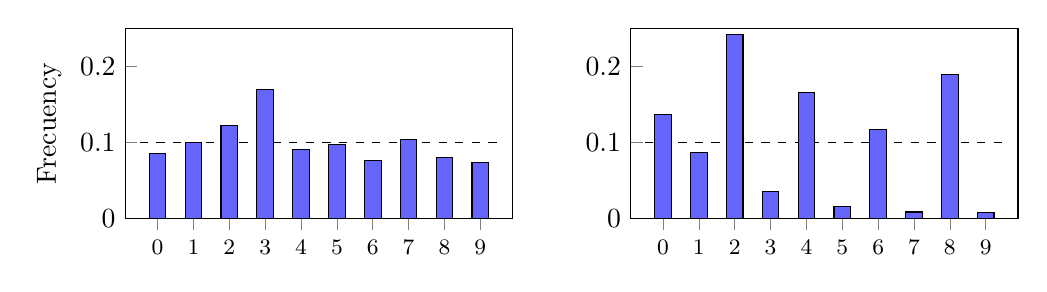
\begin{tikzpicture}
  %–––––––––––––––––––––––––––––––––––––––––––––––––––––––––––––––––––––––––
  % First plot (Run A)
  %–––––––––––––––––––––––––––––––––––––––––––––––––––––––––––––––––––––––––
  \begin{axis}[
      name=plotA,
      ybar,
      bar width=6pt,
      width=6.5cm, height=4cm,
      enlarge x limits=0.1,
      ymin=0, ymax=0.25,
      %title={Run A},
      ylabel={Frecuency},
      xtick={0,...,9},
      xticklabel style={font=\footnotesize},
      axis lines=box,
      % ensure ticks appear on bottom & left only
      xtick pos=bottom,
      ytick pos=left,
    ]
    % horizontal line at y=0.1
    \draw[black, dashed] 
      (axis cs:-0.5,0.1) -- (axis cs:9.5,0.1);
    % bars
    \addplot[fill=blue!60] coordinates {
      (0,0.086) (1,0.0996) (2,0.1223) (3,0.1694) (4,0.0904)
      (5,0.0979) (6,0.0762) (7,0.1034) (8,0.0806) (9,0.0742)
    };
  \end{axis}

  %–––––––––––––––––––––––––––––––––––––––––––––––––––––––––––––––––––––––––
  % Second plot (Run B), shifted right by 8cm
  %–––––––––––––––––––––––––––––––––––––––––––––––––––––––––––––––––––––––––
  \begin{axis}[
      at={(plotA.south east)},    % anchor to the right of the first
      anchor=south west,          % align by their south west/east corners
      xshift=1.5cm,               % small gap
      ybar,
      bar width=6pt,
      width=6.5cm, height=4cm,
      enlarge x limits=0.1,
      ymin=0, ymax=0.25,
      %title={Run B},
      %ylabel={Value},
      xtick={0,...,9},
      xticklabel style={font=\footnotesize},
      % only draw bottom and left axes
      axis lines=box,
      % ensure ticks appear on bottom & left only
      xtick pos=bottom,
      ytick pos=left,
    ]
    \draw[black, dashed] 
      (axis cs:-0.5,0.1) -- (axis cs:9.5,0.1);
    \addplot[fill=blue!60] coordinates {
      (0,0.1372) (1,0.0864) (2,0.2413) (3,0.036) (4,0.1659)
      (5,0.0155) (6,0.1171) (7,0.0087) (8,0.1895) (9,0.0078)
    };
  \end{axis}
\end{tikzpicture}
  \caption{Class‐frequency distributions of MNIST samples generated by two different models. Left: dual-ISL; Right: standard DCGAN. Each bar represents the proportion of generated images assigned to each digit class (0–9), illustrating that dual-ISL produces a more uniform coverage across all classes, whereas the DCGAN exhibits notable biases toward certain digits. The dashed line indicates the ideal uniform distribution across all classes.}
  \label{fig:digits frequency}
\end{figure}

\begin{figure}[htb!]
  \centering
  \begin{subfigure}[t]{0.48\textwidth}
    \centering
    \includegraphics[width=\linewidth, height=5cm]{img/high_dim/precision_m20_m100_MNIST.pdf}
    %\caption{Dual Moon}
    \label{fig:precision_m20_m100_MNIST}
  \end{subfigure}
  \hfill
  \begin{subfigure}[t]{0.48\textwidth}
    \centering
    \includegraphics[width=\linewidth, height=5cm]{img/high_dim/recall_m20_m100_MNIST.pdf}
    %\caption{}
    \label{fig:recall_m20_m100_MNIST}
  \end{subfigure}

  \vspace{0.5ex}
  \caption{Precision (left) and recall (right) on the MNIST test set after 50 training epochs, using $m=20$ and $m=100$ random projections.}
  \label{fig:ablation studies on p and r metrics vs m}
\end{figure}

\begin{figure}[htb!]
  \centering
  \begin{subfigure}[t]{0.48\textwidth}
    \centering
    \includegraphics[width=\linewidth, height=5cm]{img/high_dim/GAN.pdf}
    \caption{DCGAN}
    \label{fig:GAN}
  \end{subfigure}
  \hfill
  \begin{subfigure}[t]{0.48\textwidth}
    \centering
    \includegraphics[width=\linewidth, height=5cm]{img/high_dim/ISL+GAN.pdf}
    \caption{DCGAN pretrained with ISL}
    \label{fig:ISL_GAN}
  \end{subfigure}

  \vspace{0.5ex}
  \caption{Figure \ref{fig:GAN} shows digits generated by a standard DCGAN, while Figure \ref{fig:ISL_GAN} shows samples from a DCGAN pretrained with ISL. The ISL-pretrained model exhibits significantly greater diversity across all classes, whereas the vanilla DCGAN produces an overabundance of ‘1’s.
}
  \label{fig:MNIST_good}
\end{figure}


\begin{figure}[htb!]
  \centering
  \begin{subfigure}[t]{0.48\textwidth}
    \centering
    \includegraphics[width=\linewidth, height=5cm]{img/high_dim/FMNIST_DCGAN.pdf}
    \caption{DCGAN}
    \label{fig:FMNIST_ISL}
  \end{subfigure}
  \hfill
  \begin{subfigure}[t]{0.48\textwidth}
    \centering
    \includegraphics[width=\linewidth, height=5cm]{img/high_dim/FMNIST_ISLDCGAN_4.pdf}
    \caption{DCGAN pretrained with ISL}
    \label{fig:FMNIST_ISLDCGAN}
  \end{subfigure}

  \vspace{0.5ex}
  \caption{Comparison of Fashion-MNIST samples: \ref{fig:FMNIST_ISL} generated by DCGAN trained 40 epochs, and \ref{fig:FMNIST_ISLDCGAN} generated by a DCGAN pretrained with dual-ISL. The ISL-pretrained model demonstrates greater class diversity and improved precision.
}
  \label{fig:FMNIST_good}
\end{figure}




\newpage\clearpage
% \subsection{Summary}

% \begin{figure}[ht!]
%   \centering
%   \fbox{%  % uncomment if you still want a frame
%   \begin{tikzpicture}[scale=3,
%       % reusable style for all region labels:
%       venn/.style={
%         align=center,       % multi-line, centered
%         text centered,      % center text block at coordinate
%         anchor=center,      % node center at coordinate
%         text width=1.5cm,   % wrap width
%         inner sep=1pt,       % small padding
%       }
%     ]

%   \definecolor{pastelbrown}{RGB}{200,160,100}
%   \definecolor{pastelblue} {RGB}{120,160,190}
%   \definecolor{pastelviolet}{RGB}{170,140,170}

%     %--- add top-left overarching label
%     \node[font=\small\itshape, anchor=south west]
%       at (-1.9,2.3) {Implicit generative models};

%     %--- circle centers & radius
%     \coordinate (A) at (-0.8, 0);
%     \coordinate (B) at ( 0.8, 0);
%     \coordinate (C) at ( 0,   1.0);
%     \def\r{1.2cm}

%     %--- draw semi-transparent sets
%     \fill[pastelbrown,   fill opacity=0.5, draw=black] (A) circle (\r);
%     \fill[pastelblue, fill opacity=0.5, draw=black] (B) circle (\r);
%     \fill[pastelviolet,  fill opacity=0.5, draw=black] (C) circle (\r);

%     %--- set‐name labels
%     \node[font=\bfseries] at ([yshift=-1.4cm]A) {NFs};
%     \node[font=\bfseries] at ([yshift=-1.4cm]B) {GANs};
%     \node[font=\bfseries] at ([yshift= 1.4cm]C) {DDPMs};

%     %--- region labels
%     \node[venn] at (-1.2,  -0.4) {\small Probability evaluation};
%     \node[venn] at ( 1.2,  -0.2) {\small Fast sampling\\ Flexible model};
%     \node[venn] at ( 0.0,  1.7) {\small Mode coverage};
%     %\node[venn] at ( 0.0,  0.0) {Invertible\\generator};
%     %\node[venn] at (-0.5,  0.8) {Likelihood\\evaluation};
%     %\node[venn] at ( 0.5,  0.8) {Implicit,\\likelihood‐free};

%     %--- central ISL label
%     \node[font=\bfseries,venn] at ( 0.0,  0.3) {ISL};

%   \end{tikzpicture}
%   }% end \fbox
%   \caption{\small Key trade‐offs among popular implicit generative paradigms. Normalizing Flows (NFs) offer explicit density evaluation, GANs enable ultra‐fast sampling, flexibel models, and DDPMs excel at mode coverage. ISL sits at their intersection, combining fast, likelihood‐free training with both explicit density and broad support coverage.}
%   \label{fig:venn2}
% \end{figure}

% \begin{figure}[ht]
%   \centering
%   \begin{venndiagram3sets}[
%       tikzoptions={scale=3,thick, line width=1pt},
%       labelA={\(NFs\)},
%       labelB={\(GANs\)},
%       labelC={\(DDPMs\)},
%       shade=blue!30,
%       labelOnlyA={Explicit density},
%       labelOnlyB={Fast sampling},
%       labelOnlyC={Mode Coverage},
%       labelOnlyAB={Fast sampling \& Explicit density},
%       labelOnlyAC={Mode Coverage \& Explicit density},
%       labelOnlyBC={Implicit, likelihood-free training},
%       labelABC={ISL},
%     ]
%     \setpostvennhook{\node[above left] at (venn top right){Implicit Generative Models};}
%   \end{venndiagram3sets}
%   \caption{How various likelihood‐based and likelihood‐free methods compare.}
%   \label{fig:venn2}
% \end{figure}


\newpage \clearpage

\section{Pseudocodes} \label{pseudocodes}
Below we summarize two variants of the dual‐ISL training procedure.  Algorithm~\ref{alg:dual-isl} presents the basic likelihood‐free, rank‐based update in the one‐dimensional case.  Algorithm~\ref{alg:dual-isl-multidim} extends this to multi‐dimensional data by drawing random one‐dimensional projections and averaging the resulting rank losses.

\begin{algorithm}[ht!]
\setstretch{1.2}
\caption{dual-ISL Training}\label{alg:dual-isl}
\begin{algorithmic}[1]
  \REQUIRE Generator network $f_{\theta}$, real samples $\{y_i\}_{i=1}^N$, batch size $M$, rank draws $K$, epochs $T$, learning rate $\eta$
  \ENSURE  Trained parameters $\theta$
  \FOR{epoch $=1$ to $T$}
    \FOR{each minibatch $B\subset \{y_i\}_{i=1}^{N}$ of size $M$}
      \STATE Sample noise $z \sim p_z$
      \STATE Generate fictious sample $\tilde y = f_\theta(z)$
      \STATE Initialize histogram $\mathbf{q} \leftarrow \mathbf{0}$
      \FOR{$t = 1,\dots,\lfloor M/K\rfloor$}
      %\FOR{ $1, \ldots, \lfloor M/K\rfloor $, select $\{y\}_{i=0}^{K}$ random samples from $B$}
        \STATE $\{y_i\}_{i=1}^{K} \gets \text{RandomSubset}(B,\,K)$  \COMMENT{draw $K$ real samples from the minibatch}
        \STATE $a_K \leftarrow \sum_{i=1}^K \mathrm{SoftIndicator}[\tilde y \le y_{i}]$ \COMMENT{differentiable count of the $A_{K}$ statistic}
        \STATE $\mathbf{q}\leftarrow \mathbf{q} + \mathrm{SoftHotEncoding}(a_K,\ \text{length}=K+1)$ \COMMENT{accumulate a differentiable one-hot into the histogram}
      \ENDFOR
      %\STATE Set uniform target $u[k] = 1/(K+1)$ for $k=0,\dots,K$
      \STATE $\mathbf{q} \leftarrow \mathrm{normalize}(\mathbf{q})$
      \STATE Compute loss: $\mathit{loss} \leftarrow \left|\left|\frac{1}{K+1}\mathbf{1}_{K+1}-\mathbf{q}\right|\right|_{\ell^1}$
      \STATE Update: $\theta \leftarrow \theta \;-\;\eta\,\nabla_{\theta}\,\mathit{loss}$
    \ENDFOR
  \ENDFOR 
  \RETURN $\theta$
\end{algorithmic}
\end{algorithm}

\begin{algorithm}[ht!]
\setstretch{1.2}
\caption{Dual‐ISL with Random Projections}\label{alg:dual-isl-multidim}
\begin{algorithmic}[1]
  \REQUIRE Generator $f_{\theta}$, real data $\{y_i\}_{i=1}^N\subset\mathbb{R}^d$, batch size $M$, rank draws $K$, projection draws $L$, epochs $T$, learning rate $\eta$
  \ENSURE  Learned parameters $\theta$
  \FOR{epoch = 1 \TO $T$}
    \FOR{each minibatch $B\subset\{y_i\}$ of size $M$}
      \STATE Sample noise $z \sim p_z$
      \STATE Generate fictious sample $\tilde y = f_\theta(z)$
      \STATE Initialize histogram $\mathbf{q} \leftarrow \mathbf{0}$
      \FOR{$\ell = 1$ \TO $L$}
        \STATE Sample random unit vector $v_\ell\sim \mathrm{Uniform}(S^{d-1})$
        \FOR{$t = 1,\dots,\lfloor M/K\rfloor$}
            \STATE $\{y_i\}_{i=1}^{K} \gets \text{RandomSubset}(B,\,K)$  \COMMENT{draw $K$ real samples from the minibatch}
            \STATE Compute projections $\tilde u = v_\ell^\top \tilde y$ and $u_i = v_\ell^\top y_i$ for all $i$
            \STATE $a_K \leftarrow \sum_{i=1}^K \mathrm{SoftIndicator}[\tilde u \le u_{i}]$ \COMMENT{differentiable count of the $A_{K}$ statistic}
            \STATE $\mathbf{q}\leftarrow \mathbf{q} + \mathrm{SoftHotEncoding}(a_K,\ \text{length}=K+1)$ \COMMENT{accumulate a differentiable one-hot into the histogram}
        \ENDFOR
        \STATE $\mathbf{q} \leftarrow \mathrm{normalize}(\mathbf{q})$
        \STATE $\mathrm{loss} \leftarrow \|\,\mathbf{q} - \tfrac{1}{K+1}\mathbf1_{K+1}\|_1$
      \ENDFOR
      \STATE Compute loss: $\mathrm{projection\_loss = \mathrm{mean}(loss)}$
      \STATE Update: $\theta \leftarrow \theta - \eta\,\nabla_\theta\,\mathrm{projection\_loss}$
    \ENDFOR
  \ENDFOR
  \RETURN $\theta$
\end{algorithmic}
\end{algorithm}

\newpage

\section{Experimental Setup}\label{Experimental Setup}
All experiments were performed on a MacBook Pro running macOS 13.2.1, equipped with an Apple M1 Pro CPU and 16 GB of RAM. When GPU acceleration was required, we used a single NVIDIA TITAN Xp with 12 GB of VRAM. Detailed hyperparameter settings for each experiment are provided in the corresponding sections. An anonymous repository containing all code and data is available at \url{https://anonymous.4open.science/r/dual-isl-6633}. The code will also be included in the supplementary materials in a folder.


\section{Limitations}

While our invariant statistical loss (ISL) framework eliminates the need for adversarial critics and guarantees strong convergence, it faces a critical trade-off when extended to high-dimensional data via ISL-slicing. Specifically, it requires $m$ random projections: a large $m$ enhances fidelity but incurs steep computational costs, whereas a small $m$ may overlook key anisotropic features. To address this, future research should design adaptive strategies for choosing or weighting projections—potentially drawing on recent advances in slicing-Wasserstein theory—to maximize information gain per projection. Moreover, exploring alternative projection methods (such as data-dependent or learned mappings) and establishing rigorous convergence bounds that link $m$  to both convergence rate and approximation error will be essential for fully automating and optimizing ISL’s performance.

By viewing ISL as the “cost” of rearranging generated samples to match real data points, we uncover its direct relationship with optimal transport. In essence, the permutation that sorts one sample set against another defines an explicit coupling—much like the Monge map—between the model and data distributions. Future work should formalize this correspondence, harnessing optimal transport tools to both analyze ISL’s theoretical properties and develop faster, more principled algorithms.



\section{Potential Societal Impact}

Implicit generative models unlock powerful data‐synthesis capabilities but also pose dual-use risks. Although our ISL framework could produce highly realistic outputs—such as photorealistic faces or authentic-sounding voices—it could likewise be misused to generate deep fakes. At the same time, we have shown that ISL excels at modeling heavy-tailed distributions, which helps ensure rare or minority subpopulations are neither over- nor under-represented. Furthermore, the closed-form density estimation inherent in ISL offers a transparent window into what is otherwise a black-box process, improving explainability and enabling practitioners to audit and adjust model behavior for fairness. By combining high-fidelity synthesis with built-in safeguards and interpretability, ISL paves the way for more responsible, equitable deployment of generative technologies.

\end{document}


